\documentclass[mathserif,10pt]{beamer}
\newcommand{\be}{\begin{equation}}
\newcommand{\ee}{\end{equation}}
\newcommand{\bce}{\begin{center}}
\newcommand{\ece}{\end{center}}
\newcommand{\dpa}[2]{\frac{\partial #1}{\partial #2}}
\newcommand{\ndp}[3]{\frac{\partial^#3 #1}{\partial #2 ^#3}}
\newcommand{\cdpa}[3]{\frac{\partial^2 #1}{\partial #2 \partial #3}}
\usepackage[utf8]{inputenc}
\usepackage{ragged2e}
\usepackage{etoolbox}
\usepackage{animate}
\usepackage{booktabs}
\usepackage{eulervm}
\apptocmd{\frame}{}{\justifying}{}
\usepackage[activeacute,spanish]{babel}
\renewcommand\spanishtablename{Tabla}
\setbeamertemplate{navigation symbols}{}
\setbeamertemplate{caption}[numbered]
\usetheme{default}
\setbeamertemplate{footline}[frame number]
\definecolor{cobalt}{rgb}{0.0, 0.28, 0.67}
\usecolortheme[named=cobalt]{structure}
\setbeamercolor{alerted text}{fg=blue}
\title{Simulación Multiescala de Viento Sobre Terreno Complejo Mediante el Método Embebido WRF-LES y Asimilación Variacional de Datos 4D}
\author{Pablo Andrés Cárdenas Zamorano}
\institute[Universidad Técnica Federico Santa María]
{%
  Magíster en Ciencias de la Ingeniería Mecánica\\
  Universidad Técnica Federico Santa María\\
  \bigskip
  \begin{tabular}{ll}
  	 Profesor Guía:& Ph.D. Alex Flores Maradiaga\\
  	 Profesor Correferente:& Ph.D. Carlos Rosales Huerta\\
  	 Evaluador Externo:& Ph.D. Ricardo Muñoz Magnino \\
  \end{tabular}
 }
\date{\footnotesize Octubre, 2019}
\AtBeginSubsection[]
{
  \begin{frame}<beamer>{Outline}
    \tableofcontents[currentsection,currentsubsection]
  \end{frame}
}
 
\begin{document}
\begin{frame}
	\vspace{0.3cm}
	\begin{center} 
\includegraphics[height=1.5cm]{utfsm_logo} \end{center}
	\vspace{-0.5cm}
	\titlepage
\end{frame}

%\begin{frame}{Contenidos}
%	%\begin{minipage}{0.5\linewidth}
%		\tableofcontents
%	%\end{minipage}%
%	%\begin{minipage}{0.5\linewidth}
%		%\tableofcontents
%	%\end{minipage}%%
%\end{frame}

\section{1. Motivación}
\begin{frame}{Motivación}{¿Por qué Predecir el Viento?}
\begin{figure}
	\centering
	\includegraphics[width=1.0\linewidth,page=30,trim={2cm 18cm 2.5cm 3cm},clip]{fig/01/Anuario-CNE-2018}
	\vspace{3mm}
	\includegraphics[width=1.0\linewidth,page=30,trim={2cm 2.5cm 2.5cm 23.1cm},clip]{fig/01/Anuario-CNE-2018}
	\vspace{3mm}
	\caption{Evolución de la matriz energética chilena. Fuente: Comisión Nacional de Energía (2018).}
\end{figure}
\end{frame}

\begin{frame}{Motivación}{¿Por qué Predecir el Viento?}
	\begin{figure}
		\centering
		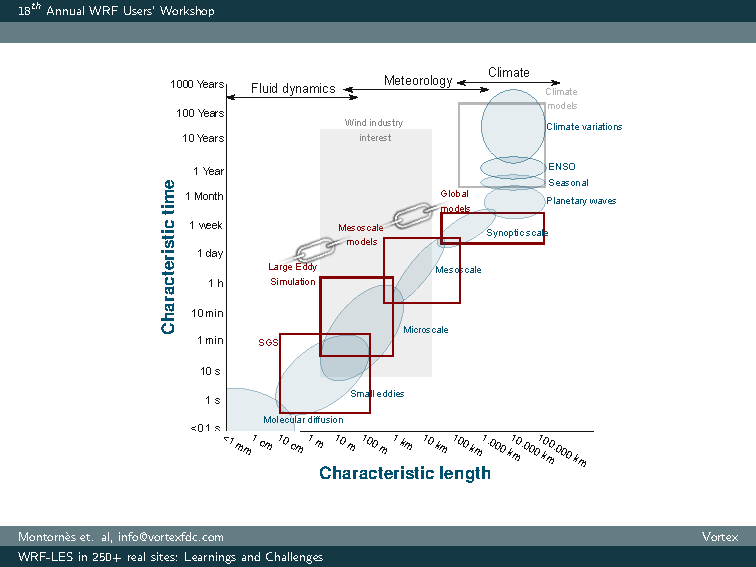
\includegraphics[width=0.7\linewidth,trim={2.6cm 1.4cm 1.5cm 0.8cm},clip]{fig/02/escalas}
		\vspace{-2mm}
		\caption{Unificación de escalas en dinámica atmosférica. Fuente: Montornes et al. (2017).}
	\end{figure}
\end{frame}

\begin{frame}{Motivación}{¿Cómo Predecirlo?}
	\begin{enumerate}[a.]
		\item Extrapolación Estadística / Simulación Numérica.
		\item Modelos Meteorológicos / CFD.
		\item Correcta representación de la CLP (PBL).
		\item Turbulencia y Terreno Complejo.
	\end{enumerate}
	\begin{figure}[h]
		\centering
		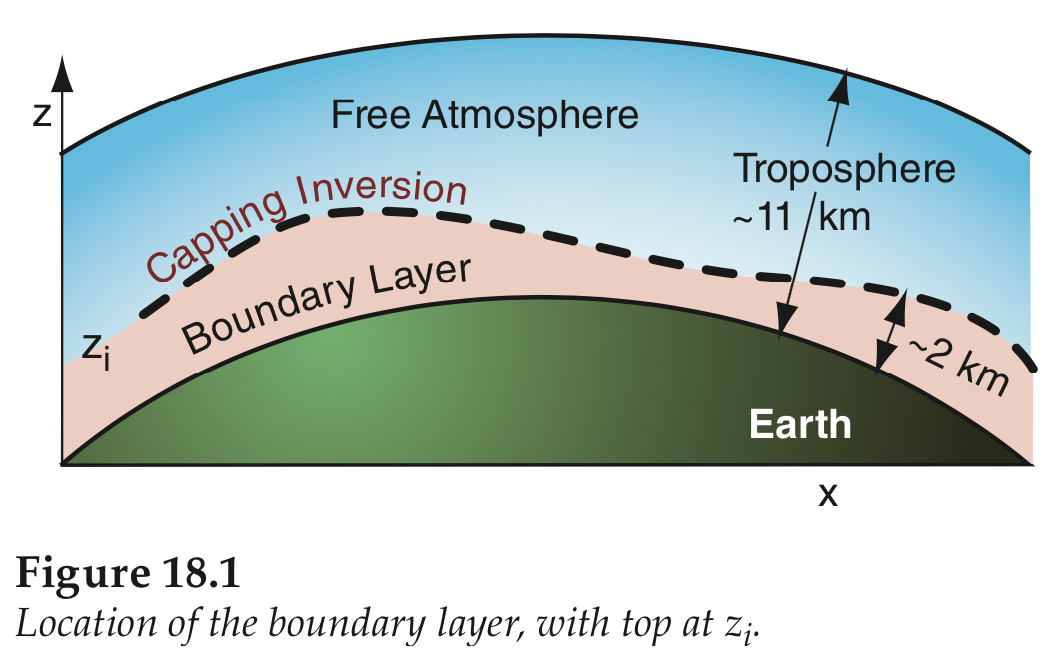
\includegraphics[width=0.7\linewidth,trim={0cm 2.5cm 0cm 0cm},clip]{fig/abl-color}
		\vspace{-4mm}
		\caption{Esquema de la capa ĺímite planetaria. Fuente: Stull (2018).}
		\label{fig:01_abl}
	\end{figure}
\end{frame}

\begin{frame}{Motivación}{¿Cómo Predecirlo?}
\begin{figure}[h]
	\centering
	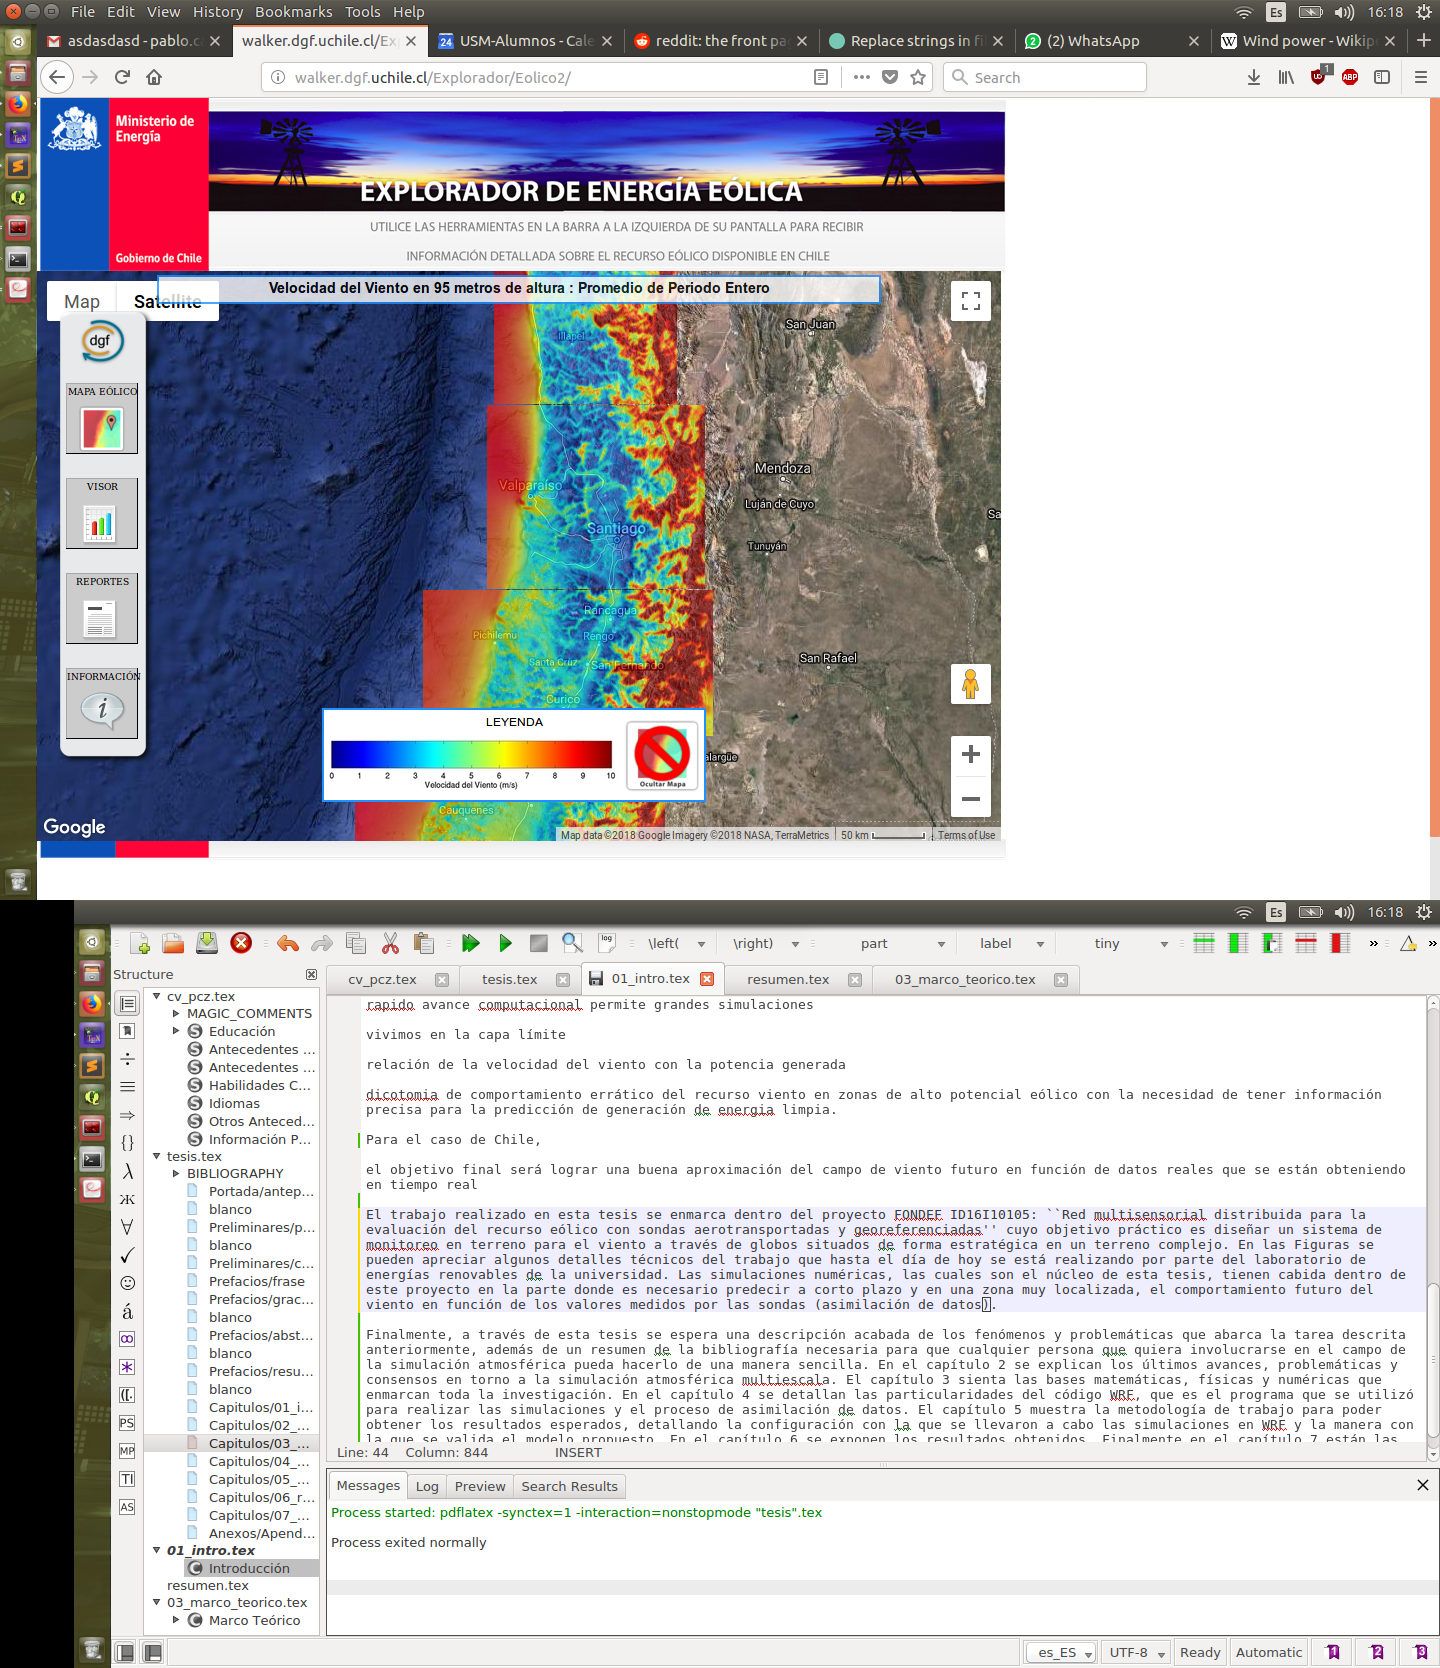
\includegraphics[width=0.8\linewidth,trim={1.4cm 28cm 15cm 3.4cm},clip]{fig/01/explo}
	\vspace{-4mm}
	\caption{Interfaz online del explorador eólico de la Universidad de Chile.}
	\label{fig:01_explorador}
\end{figure}
\end{frame}

\begin{frame}{Motivación}{¿Cómo Predecirlo?}
	\begin{figure}[h]
		\begin{minipage}{0.5\linewidth}
		\centering
		\includegraphics[width=1.0\linewidth,page=5,trim={5cm 9cm 2.3cm 3cm},clip]{fig/01/descrp}
		\end{minipage}%
		\begin{minipage}{0.5\linewidth}
			\centering
			\includegraphics[width=0.9\linewidth,page=5,trim={3cm 2.5cm 5cm 18.5cm},clip]{fig/01/descrp}
		\end{minipage}%
		\caption{Esquema de la sonda FONDEF ID16I10105.}
		\label{fig:01_sonda}
	\end{figure}
\end{frame}

\begin{frame}{Motivación}{¿Cómo Predecirlo?}
	\begin{figure}
		\begin{minipage}{0.5\linewidth}
			\centering
			(a)
		\end{minipage}%
		\begin{minipage}{0.5\linewidth}
			\centering
			(b)
		\end{minipage}%
		
		\begin{minipage}{0.5\linewidth}
			\centering
			\includegraphics[width=0.9\linewidth,page=3,trim={6cm 12.2cm 6cm 9.5cm},clip]{fig/01/descrp}
		\end{minipage}%
		\begin{minipage}{0.5\linewidth}
			\centering
			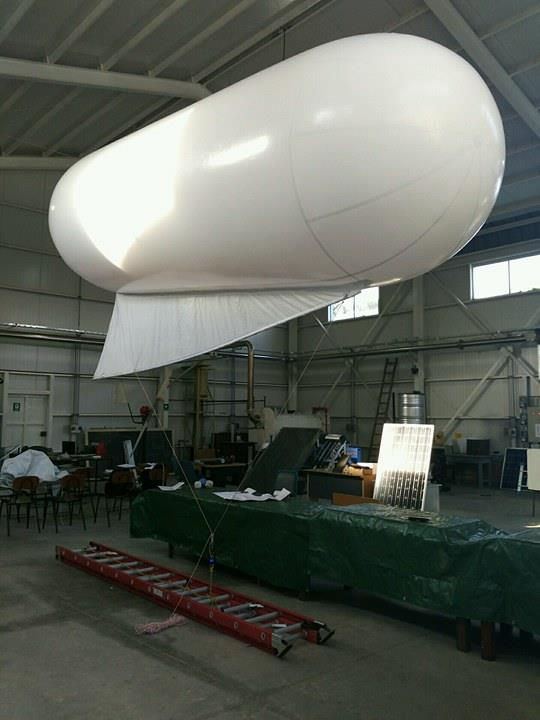
\includegraphics[width=0.7\linewidth,trim={0cm 0cm 0cm 0cm},clip]{fig/01/prototipo}
		\end{minipage}%
		\caption{Detalle del proyecto FONDEF ID16I10105. (a) Célula del sistema experimental de medición. (b) Prototipo en el laboratorio.}
		\label{fig:01_detalle_fondef}
	\end{figure}
\end{frame}

\section{2. Hipótesis y Objetivos}
\begin{frame}{Hipótesis y Objetivos}
	\begin{block}{Hipótesis}\justifying
		Se pueden mejorar las predicciones numéricas de viento a corto plazo sobre terreno complejo a través de simulaciones multiescala de alta resolución, LES y asimilación de datos 4D en la CLP.
	\end{block}
	\begin{block}{Objetivo Principal}\justifying
		Implementar una metodología que incorpore escalamiento dinámico de dominios, nuevas bases de datos de alta resolución, LES y asimilación de datos 4D multipunto para mejorar los resultados de modelos numéricos de viento sobre terreno complejo.
	\end{block}
\end{frame}

\section{3. Estado del Arte}
\begin{frame}{Estado del Arte}
	\begin{enumerate}[a.]
		\item Problemáticas del escalamiento dinámico.
		\item Antecedentes de turbulencia atmosférica y terreno complejo.
		\item Desafios de la alta resolución en terreno complejo.
		\item Contexto de la asimilación de datos.
	\end{enumerate}
\end{frame}

\begin{frame}{Estado del Arte}{Problemáticas del escalamiento dinámico}
	\begin{figure}
		\centering
		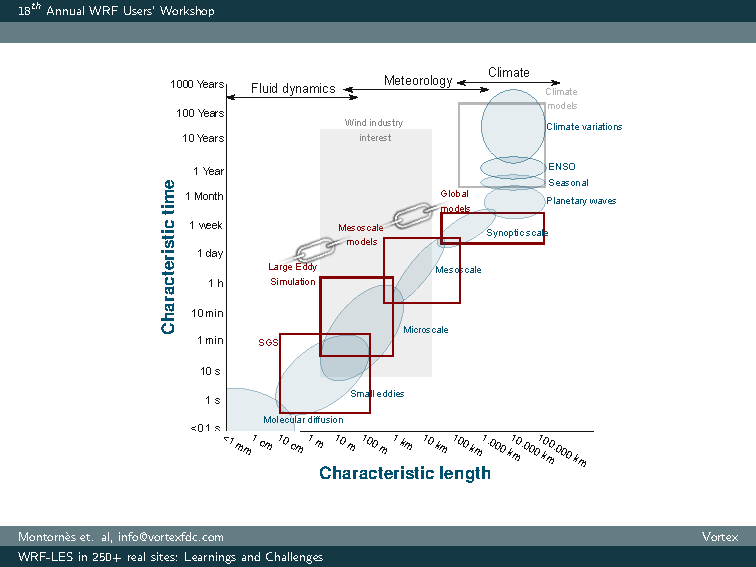
\includegraphics[width=0.7\linewidth,trim={2.6cm 1.4cm 1.5cm 0.8cm},clip]{fig/02/escalas}
		\vspace{-2mm}
		\caption{Unificación de escalas en dinámica atmosférica. Fuente: Montornes et al. (2017).}
	\end{figure}
\end{frame}

\begin{frame}{Estado del Arte}{Problemáticas del escalamiento dinámico}
	\begin{figure}
		\centering
		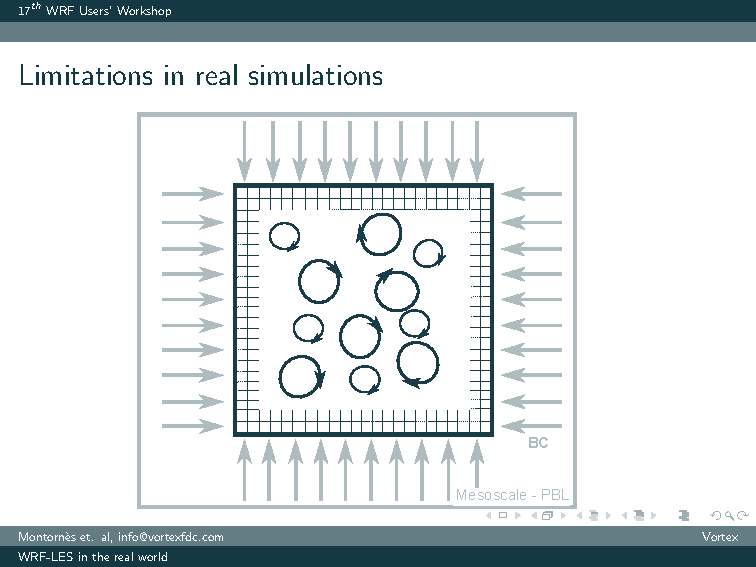
\includegraphics[width=0.6\linewidth,trim={2.67cm 1.35cm 3.1cm 2.25cm},clip]{fig/02/grid}
		\caption{Idealización de los distintos tamaños de vórtices dentro de un dominio en la zona gris de la turbulencia. Fuente: Montornes et al. (2017).}
		\label{fig:02_grid_vortex}
	\end{figure}
\end{frame}

\begin{frame}{Estado del Arte}{Problemáticas del escalamiento dinámico}
	\begin{figure}
		\centering
		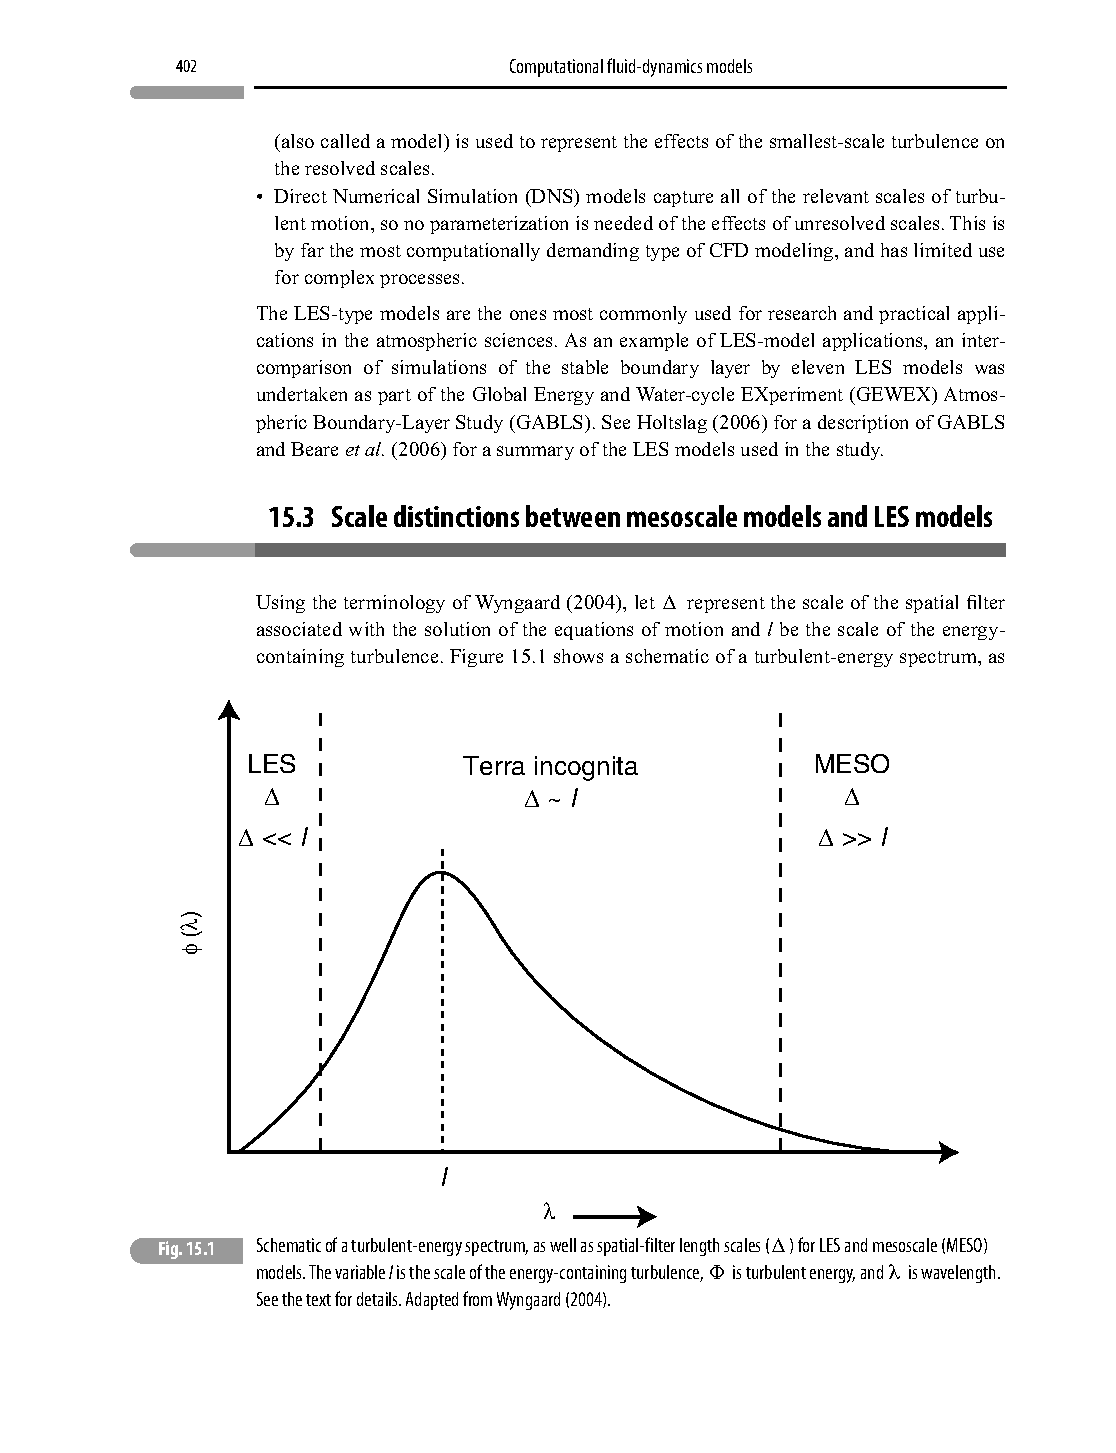
\includegraphics[width=0.9\linewidth,trim={2cm 3.0cm 1.5cm 11.5cm},clip]{fig/02/terra_inc}
		\caption{Espectro de energía cinética turbulenta multiescala. Fuente: Warner (2010).}
		\label{fig:02_terra_inc}
	\end{figure}
\end{frame}

\begin{frame}{Estado del Arte}{Turbulencia Atmosférica y Terreno Complejo}
	\begin{itemize}
		\item Modelos Lineales (Jackson y Hunt 1975, Mason y Sykes 1979)
		\item No lineales: 2D (Taylor 1977), RANS (Launder y Spalding 1974)
		\item LES: Desde los 90s se viene desarrollando para la CLP.
		\item Simulaciones Askeverin (2009) y cerros sinusoidales (2001).
	\end{itemize}
\end{frame}

\begin{frame}{Estado del Arte}{Alta Resolución y Terreno Complejo}
	\begin{itemize}
		\item Aspectos Computacionales.
		\item Aspectos Numéricos.
		\begin{itemize}
			\item Precisión
			\item Estabilidad
			\item Difusión Numérica
			\item Coordenadas
			\item Benchmarking
		\end{itemize}
		\item Parametrización de CLP.
		\item Inicialización y Datos de Entrada.
	\end{itemize}
\end{frame}

\begin{frame}{Estado del Arte}{Alta Resolución y Terreno Complejo}
	\begin{figure}[h!]
		\centering
		\vspace{0.2cm}
		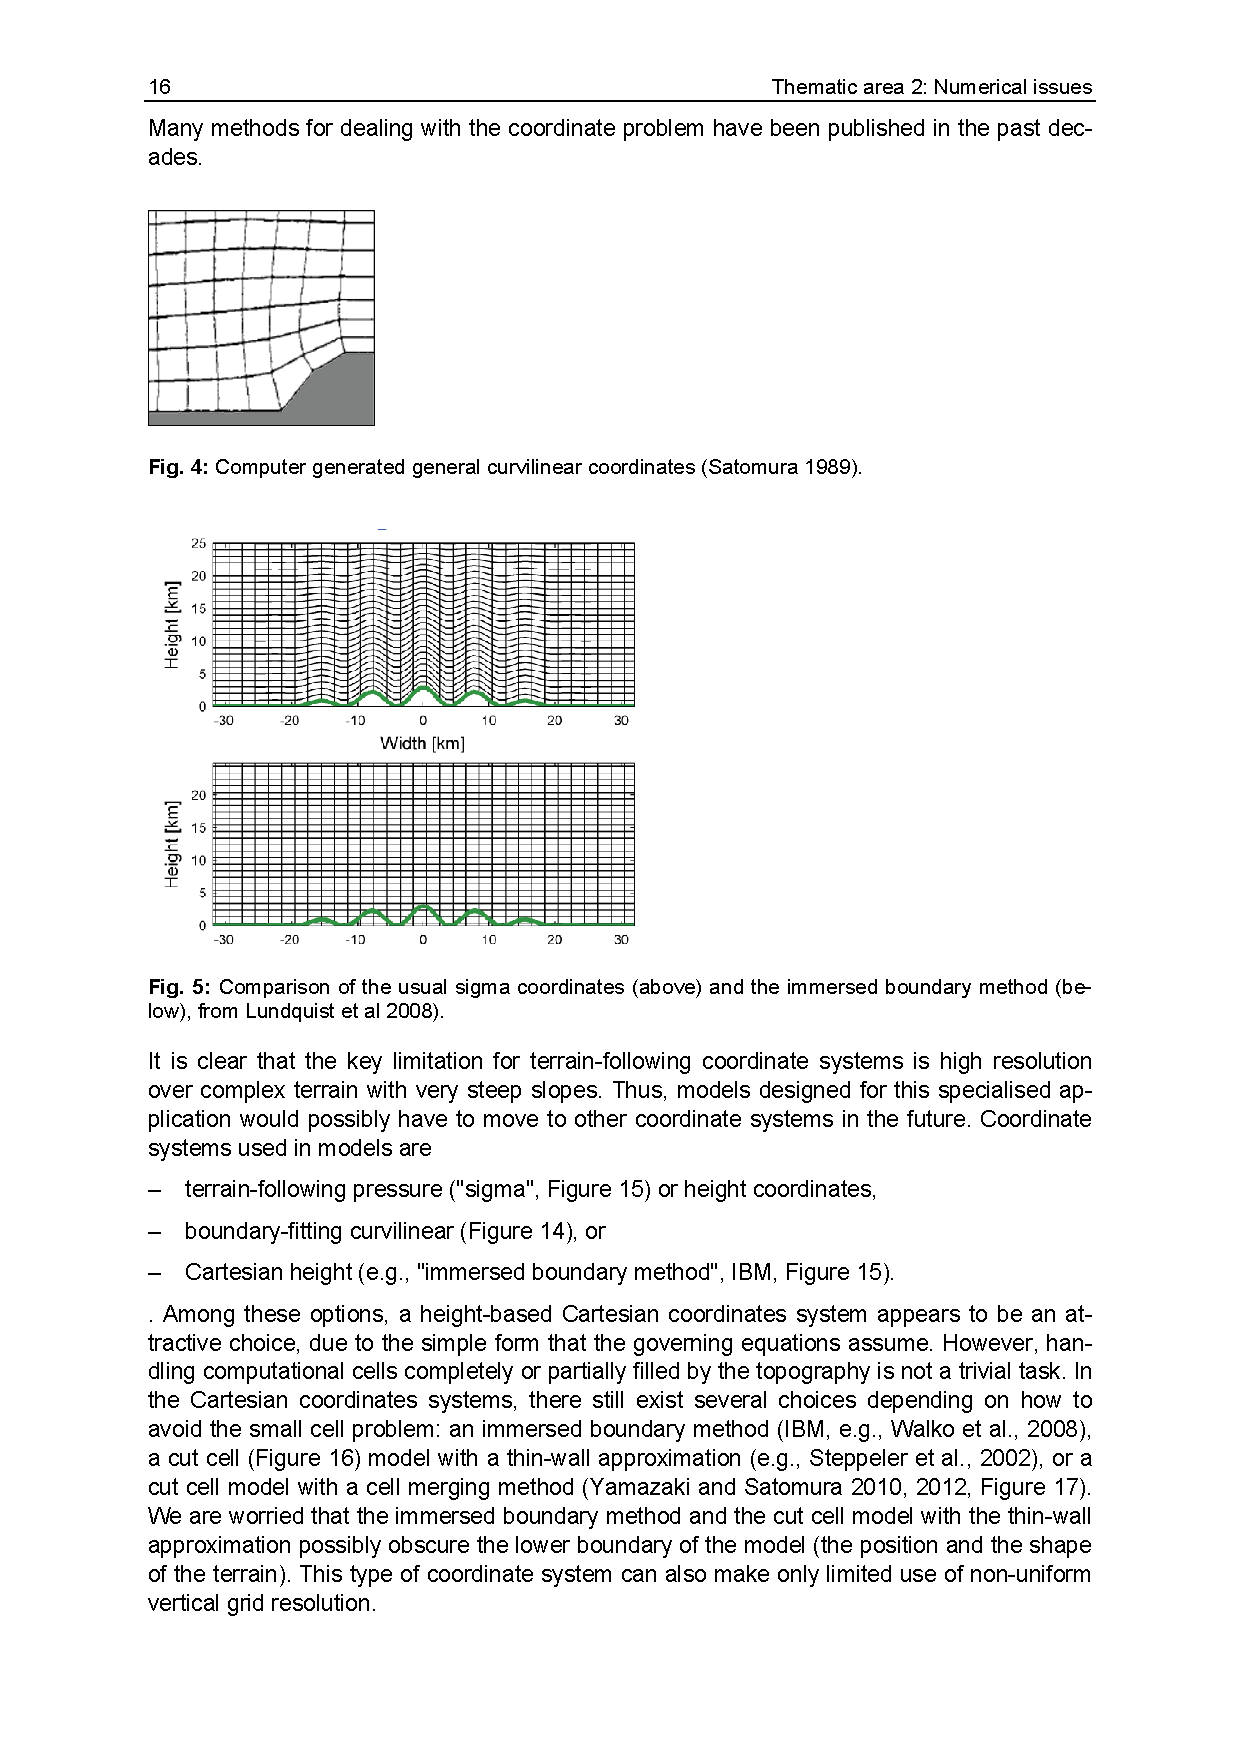
\includegraphics[width=0.75\linewidth,trim={2.6cm 13.5cm 9.2cm 9cm},clip]{fig/02/coordinates}
		\caption{Comparación entre las coordenadas usuales sigma (arriba) y el método de frontera inmersa (abajo). Fuente: Arnold et al. (2010).}
	\end{figure}
\end{frame}

\begin{frame}{Estado del Arte}{Alta Resolución y Terreno Complejo}
	\begin{itemize}
		\item Aspectos Computacionales.
		\item Aspectos Numéricos.
		\begin{itemize}
			\item Precisión
			\item Estabilidad
			\item Difusión Numérica
			\item Coordenadas
			\item Benchmarking
		\end{itemize}
		\item Parametrización de CLP.
		\item Inicialización y Datos de Entrada.
	\end{itemize}
\end{frame}

\begin{frame}{Estado del Arte}{Contexto de la Asimilación de Datos}
	\begin{itemize}
		\item Busca obtener una mejor solución mediante la combinación de observaciones con los resultados de un modelo.
		\item Es satisfactorio para los casos de escalas planetarias y sinópticas.
		\item Para la Capa Límite Planetaria (CLP) se tienen 3 casos:
		\begin{enumerate}[a.]
			\item DA en CLP para mesoescala: Mejoras de hasta un 30\% en el error.\footnote{Cheng et al. (2017) y Dumais et al. (2013)}
			\item DA con datos superficiales: Mejoras en los resultados debido al cálculo de flujos turbulentos\footnote{Stauffer et al. (1991) y Reen y Stauffer (2010)}. No para terreno complejo.
			\item \textcolor{red}{DA en CLP para microescala: No existe literatura.}
		\end{enumerate}
	\end{itemize}
\end{frame}












%MARCO TEÓRICO
\section{4. Marco Teórico}
\begin{frame}{Marco Teórico}
	\begin{enumerate}[a.]
		\item Leyes fundamentales de un Fluido.
		\item Ecuaciones que rigen la Dinámica Atmosférica.
		\item Turbulencia.
		\item Fundamentos de Capa Límite Atmosférica.
		\item Simulación de Grandes Vórtices.
		\item Asimilación de Datos.
	\end{enumerate}
\end{frame}

\begin{frame}{Marco Teórico}{Leyes Fundamentales de un Fluido}
	Conservación de Masa:
	\be \partial_t \rho + \partial_i(\rho u_i) = 0 \ee
	Conservación de Momentum:
	\be \rho d_t u_i = \rho g_i + \partial_j\sigma_{ij} \ee
	Conservación de Energía:
	\be \rho d_t\left( e+ K \right) = u_i\rho g_i + \partial_j(u_i \sigma_{ij}) - \partial_j q_i \ee
	Ecuación de Estado:
	\be p = f(\rho,T) \ee
\end{frame}
%

\begin{frame}{Marco Teórico}{Ecuaciones de Dinámica Atmosférica}
	Ecuaciones Primitivas:
	\small
	\begin{align}
	d_t u &= \frac{uv\tan\psi}{a}-\frac{uw}{a}-\frac{1}{\rho}\partial_x p - 2\Omega_e(w\cos\psi - v\sin\psi) + F_{rx}\\
	d_t v &= -\frac{u^2\tan\psi}{a}-\frac{uw}{a}-\frac{1}{\rho}\partial_y p - 2\Omega_e u\sin\psi + F_{ry}\\
	d_t w &= \frac{u^2 + v^2}{a}-\frac{1}{\rho}\partial_z p + 2\Omega_e u\cos\psi -g + F_{rz}\\
	\partial_t T &= -u\partial_x T -v\partial_y T + (\gamma-\gamma_d)w+\frac{1}{C_p}d_t H\\
	d_t \rho &= -\rho(\partial_i u_i)\\
	d_t q_v &= Q_v\label{03_eq:humedad}\\
	p &= \rho R T.
	\end{align}
	\normalsize
\end{frame}

\begin{frame}{Marco Teórico}{Ecuaciones de Dinámica Atmosférica}
	Algunas definiciones nuevas:
	\begin{itemize}
		\item Temperatura Potencial:
		\be \theta = T\left( \frac{p_s}{p} \right)^{R/C_p} \ee
		\item Temperatura Potencial Virtual:
		\be \theta_v = \theta(1+0.61q_v) \ee
		\item Criterios de Estabilidad:
		\begin{align}
		d_z \theta_v &> 0\quad;\quad\text{Estable}\label{eq:03_esta1}\\
		d_z \theta_v &= 0\quad;\quad\text{Neutra} \label{eq:03_esta2}\\
		d_z \theta_v &< 0\quad;\quad\text{Inestable} \label{eq:03_esta3}
		\end{align}
	\end{itemize}
\end{frame}
%


\begin{frame}{Marco Teórico}{Turbulencia}
	\begin{figure}[h!]
		\centering
		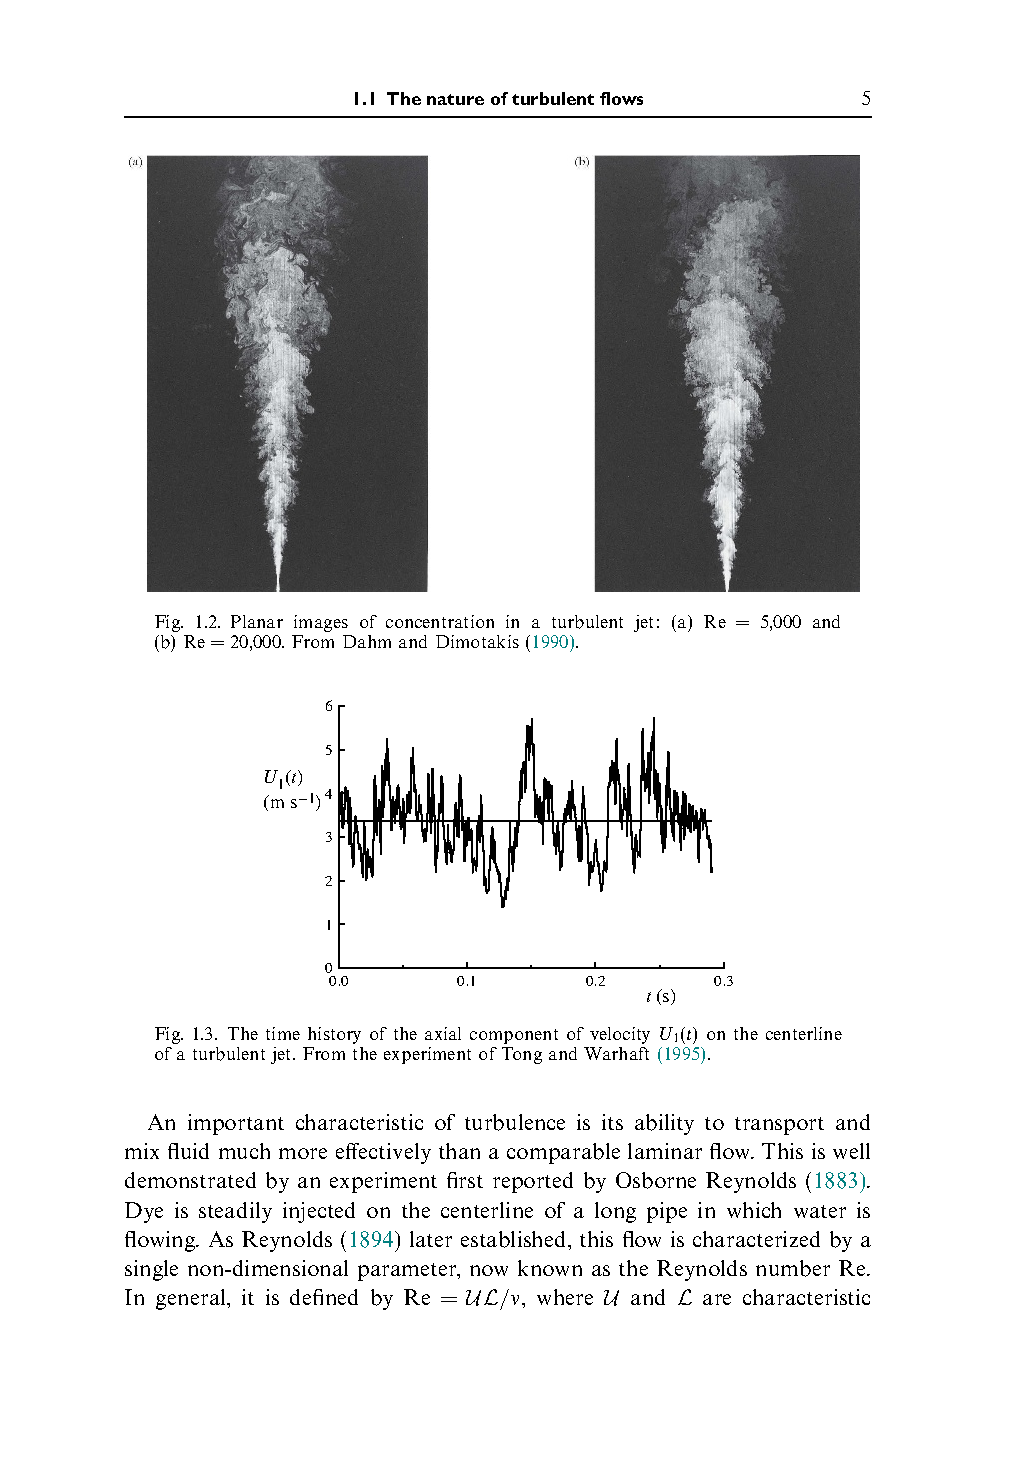
\includegraphics[width=0.8\linewidth,trim={4.3cm 7.7cm 4cm 11.5cm},clip]{fig/03/turbulent}
		\caption{Serie de tiempo para una componente de la velocidad en un flujo turbulento. Fuente: Pope (2000).}
		\label{fig:03_turbulent}
	\end{figure}
\end{frame}

\begin{frame}{Marco Teórico}{Turbulencia}
	\begin{itemize}
		\item Descomposición de Reynolds:
		\be u_i = \overline{u}_i + u'_i. \ee
		\item Ecuación de N-S promediada:
		\be
		(\partial_t \overline{u}_i + \overline{u}_j\partial_j \overline{u}_i)= \nu\partial_{jj}\overline{u}_i -\frac{1}{\rho}\partial_i \overline{p} - \partial_i(\overline{u'_iu'_j}).
		\ee
		\item Energía cinética turbulenta:
		\be k=\frac{1}{2}\overline{u'_i u'_i}. \ee
	\end{itemize}
\end{frame}

\begin{frame}{Marco Teórico}{Turbulencia}
	\begin{figure}[h!]
		\centering
		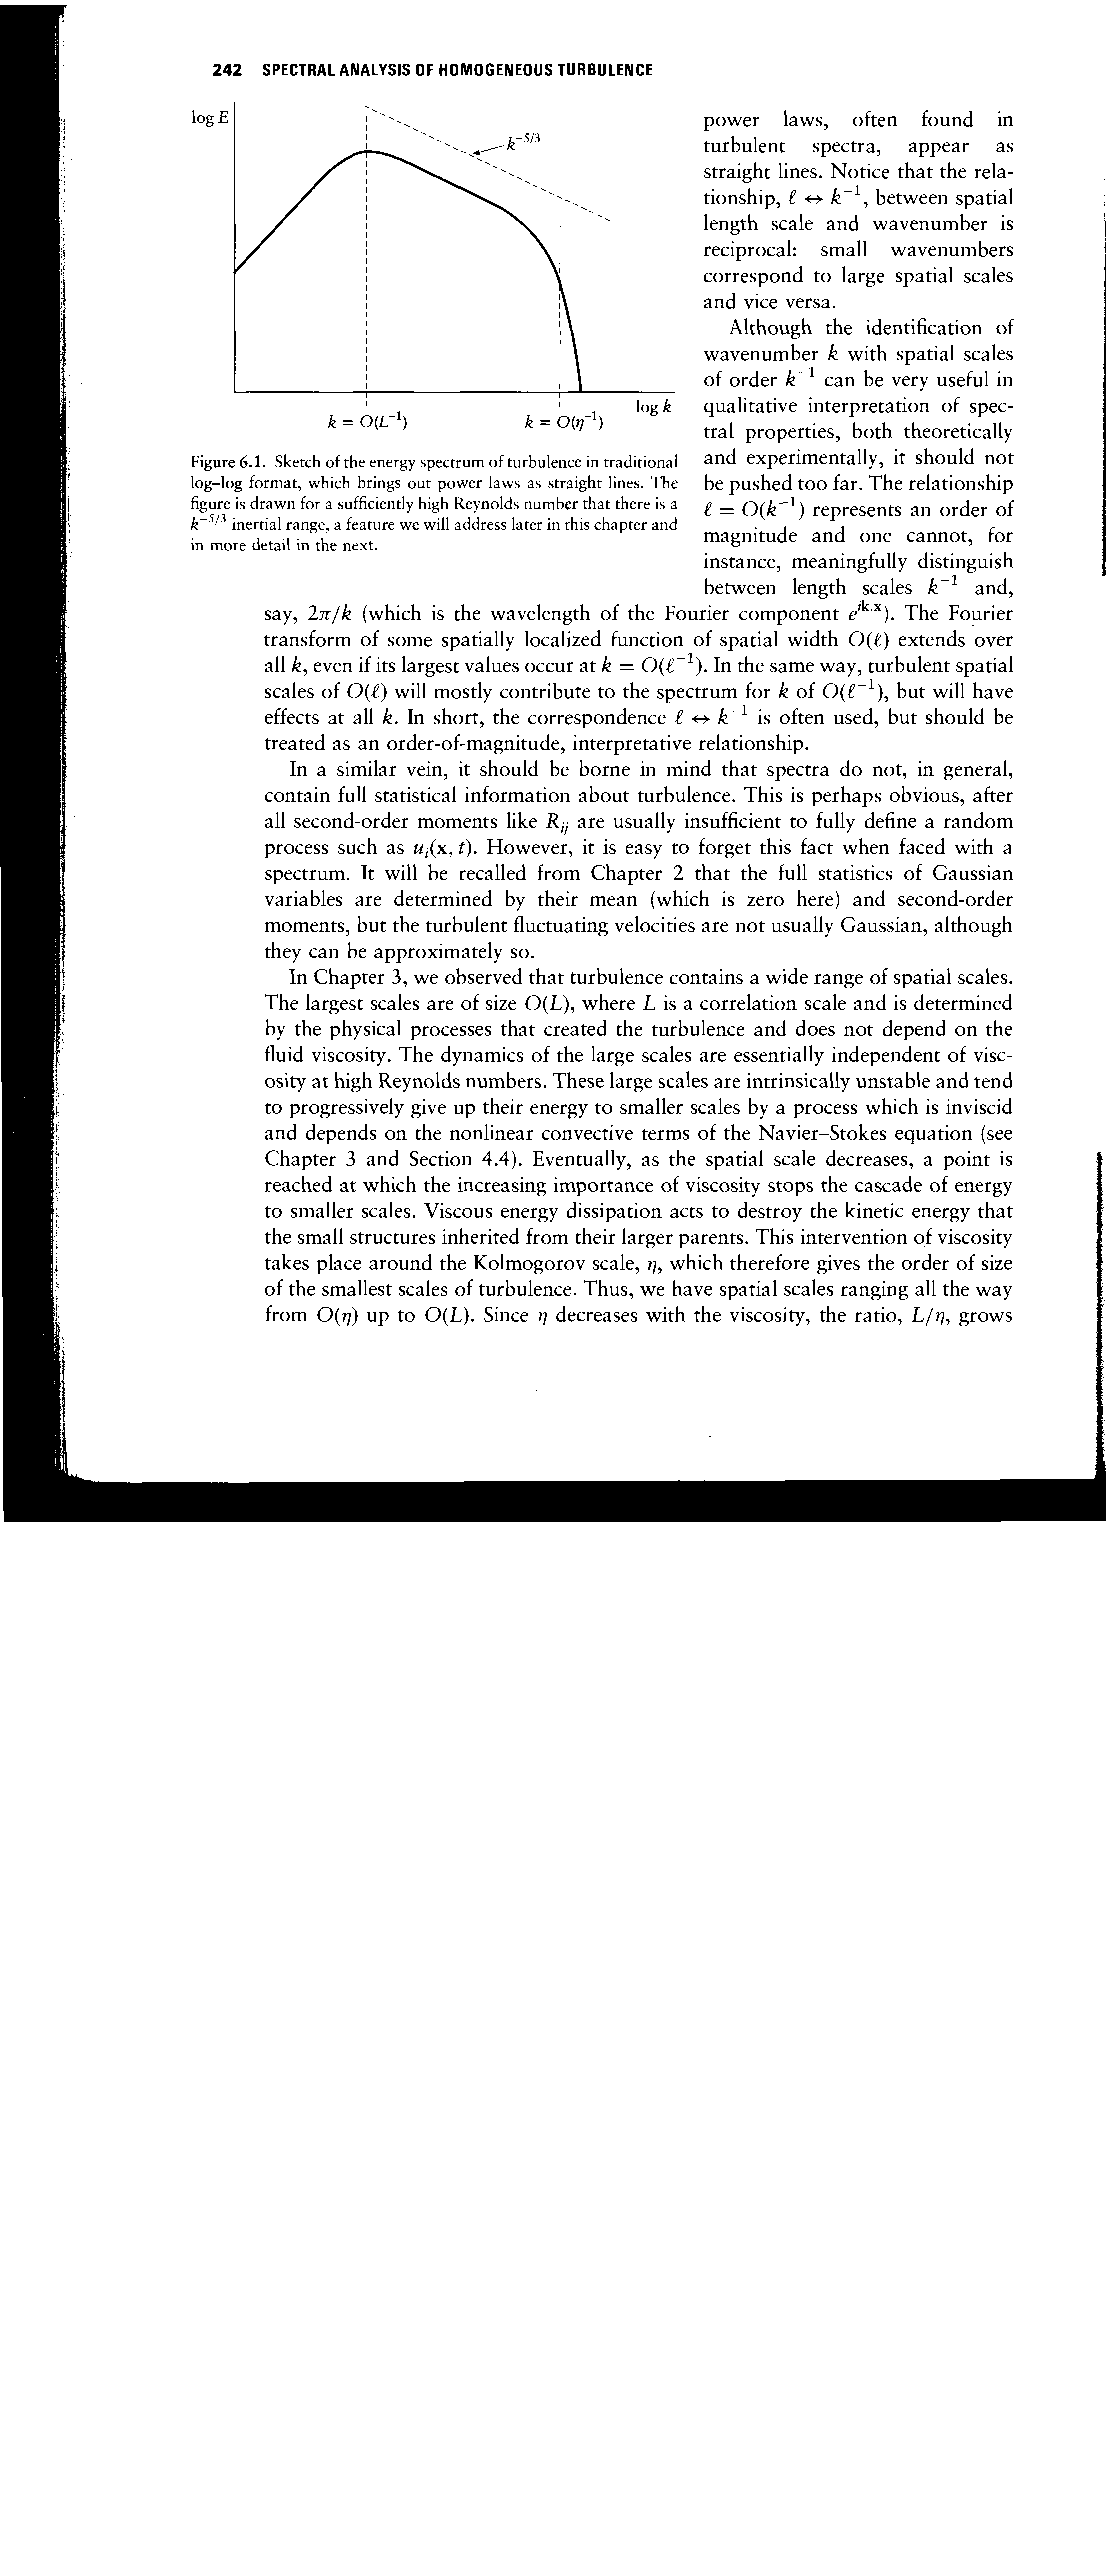
\includegraphics[width=0.75\linewidth,trim={3.2cm 18.3cm 7.0cm 1.5cm},clip]{fig/03/spectra}
		\caption{Gráfico típico log-log de distribución de energía cinética turbulenta con respecto al número de onda $\kappa$ para un flujo con un número de Reynolds elevado. Fuente: Mathieu y Scott (2000).}
		\label{fig:03_spectra}
	\end{figure}
\end{frame}

\begin{frame}{Marco Teórico}{Fundamentos de CLA}
	\begin{figure}[h!]
		\centering
		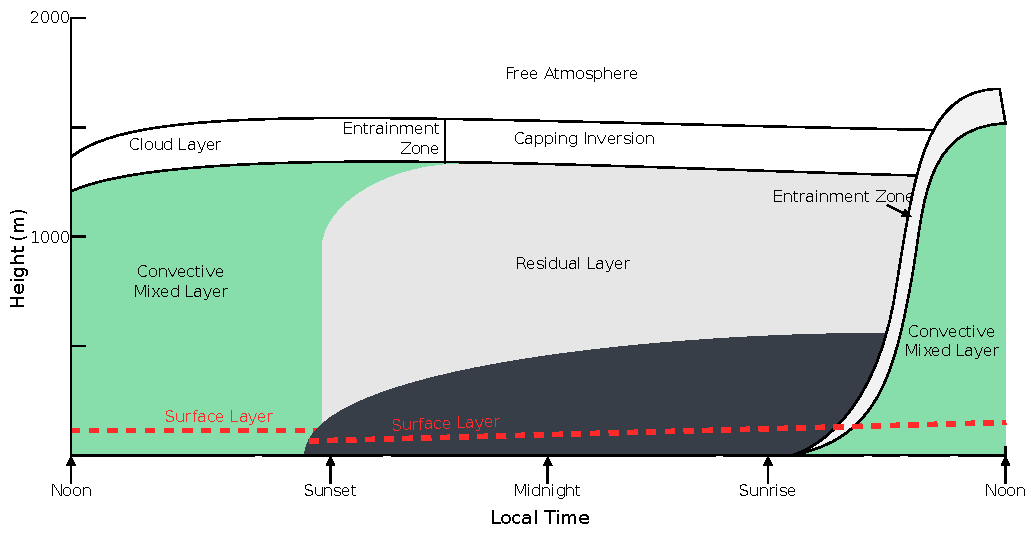
\includegraphics[width=0.98\linewidth,trim={0cm 0cm 0cm 0cm},clip]{fig/03/abl}
		\caption{Evolución diurna de la estructura de la capa límite. Fuente: Wikimedia.}
		\label{fig:03_abl}
	\end{figure}
\end{frame}

\begin{frame}{Marco Teórico}{Fundamentos de CLA}
	Principales características de la CLA:
	\begin{itemize}
		\item La humanidad gasta la mayoría de su vida dentro de la ABL.
		\item Los pronósticos del clima son en verdad pronósticos de la capa límite.
		\item La polución queda atrapada en la ABL.
		\item La neblina es creada en la ABL.
		\item La fuente principal de energía para toda la atmósfera es la radiación solar, la cual, en su mayoría es absorbida por el suelo y transmitida al resto de la atmósfera por los procesos de capa límite.
		\item Cerca de un 50\% de la energía cinética de la atmósfera es disipada en la capa límite.
		\item El transporte turbulento de momentum desde la capa límite a la superficie es el sumidero más grande de momentum de la atmósfera.
		\item Las turbinas eólicas extraen energía de los vientos de la ABL.
	\end{itemize}
\end{frame}

\begin{frame}{Marco Teórico}{Fundamentos de CLA}
	\begin{figure}[h!]
		\centering
		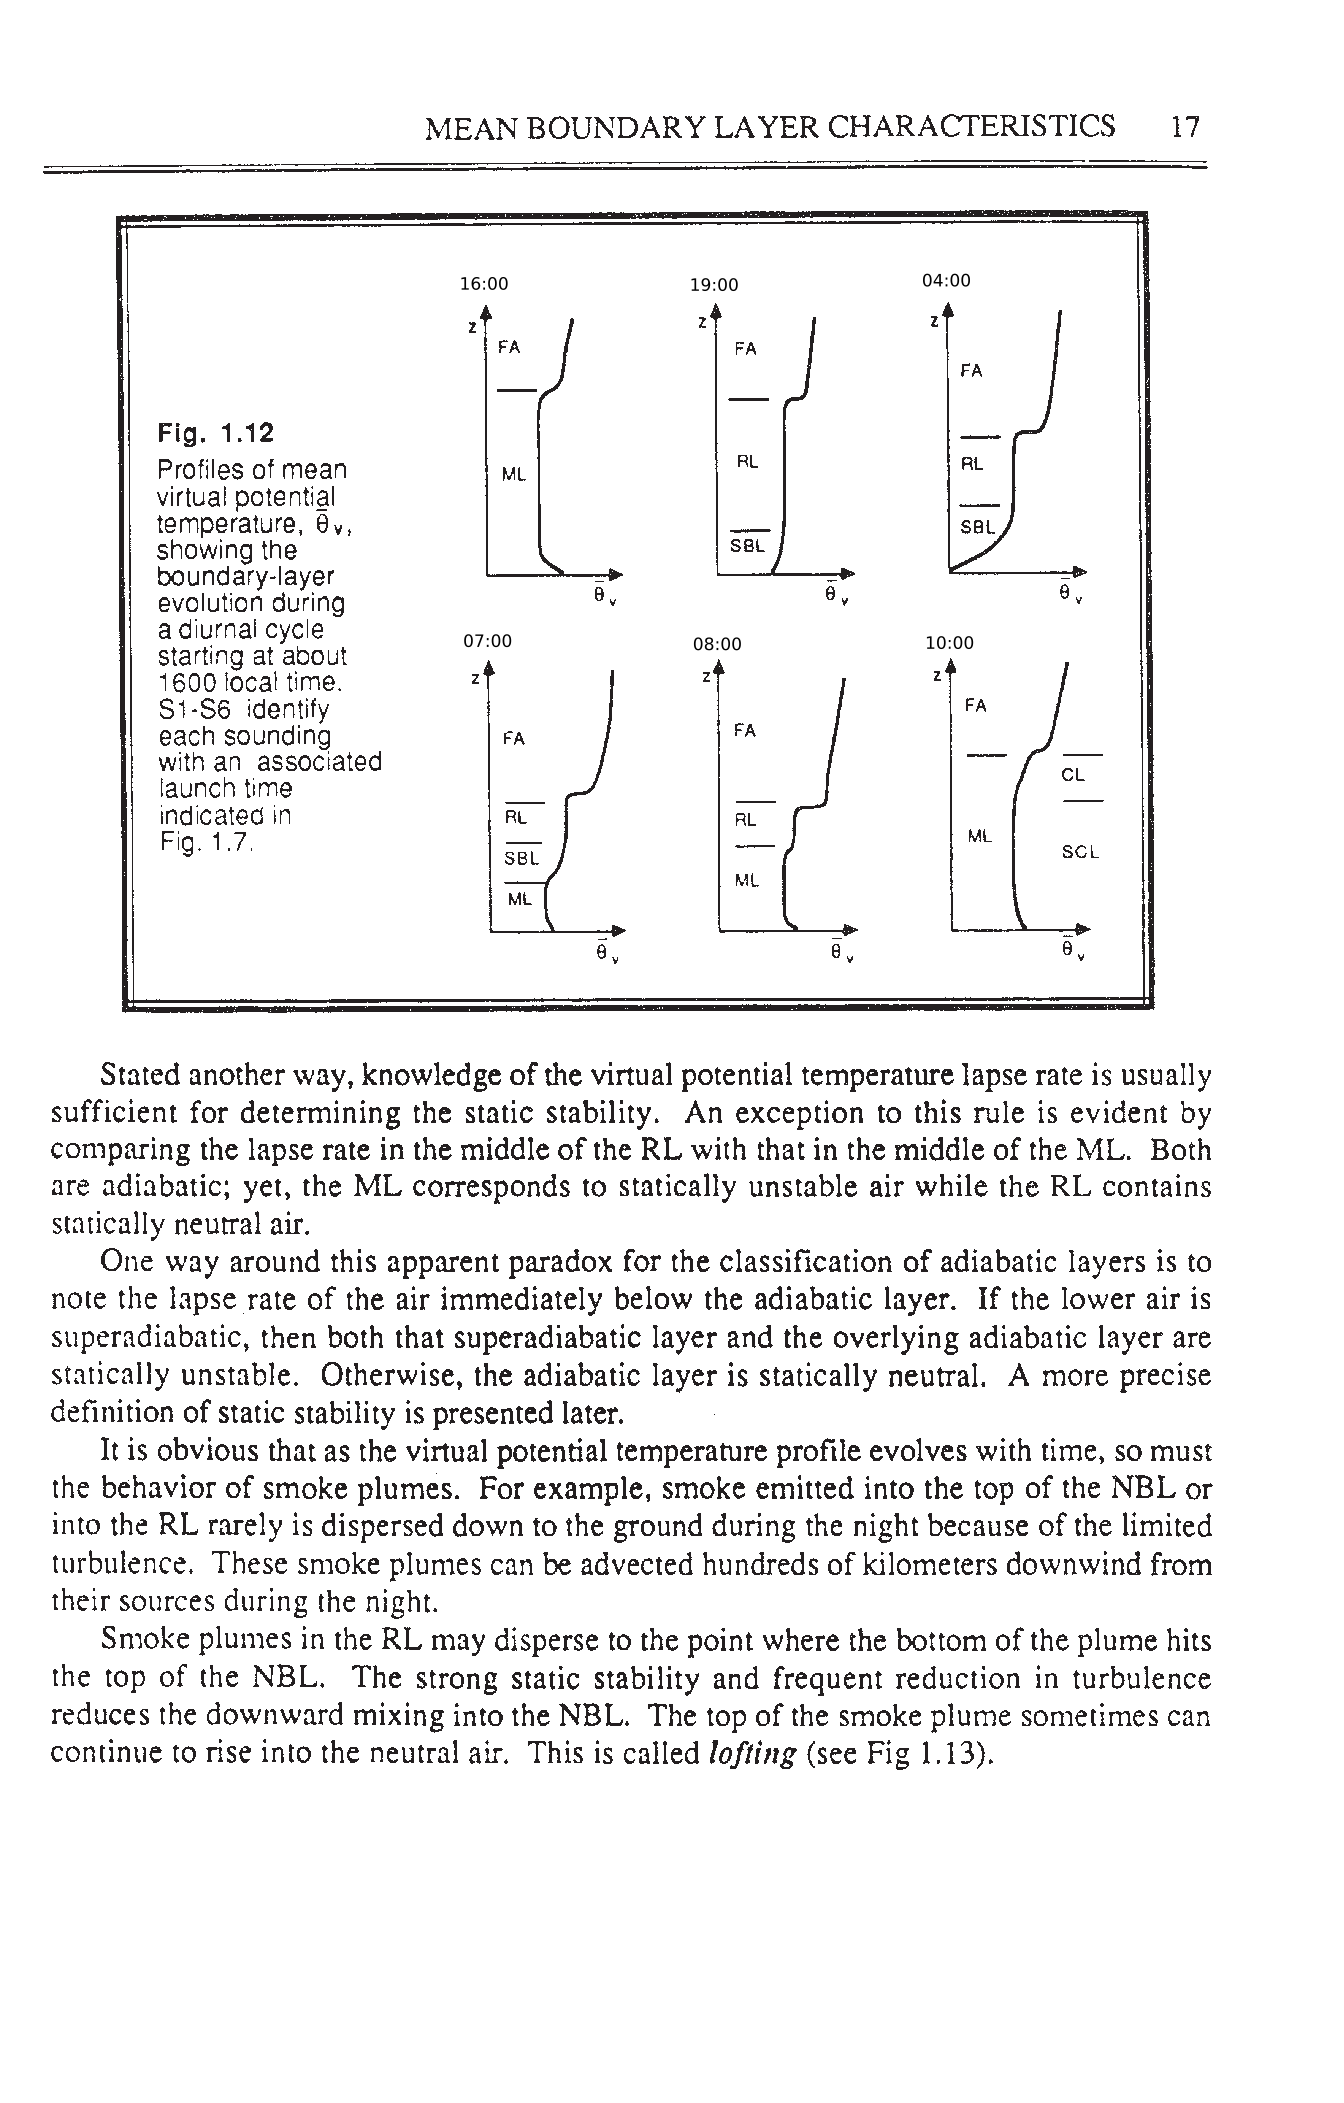
\includegraphics[width=0.6\linewidth,trim={5.6cm 14cm 2.7cm 3.3cm},clip]{fig/03/pbl2}
		\caption{Evolución del perfil de $\theta_v$ en el ciclo diurno. Fuente: Stull (1988).}
		\label{fig:03_pbl2}
	\end{figure}
\end{frame}

\begin{frame}{Marco Teórico}{Fundamentos de CLA}
Definimos nuevas variables relevantes:
	\begin{itemize}
		\item Esfuerzo (turbulento) Superficial:
		\be 
		\tau^r_{xz,s} = - \rho (\overline{w'u'})_s
		\ee
		\item Velocidad de Fricción:
		\be u_* = \sqrt{\frac{\tau^r_{xz,s}}{\rho}} \ee
	\end{itemize}
Se debe encontrar una clausura para $\tau^r_{xz}$. Existen varios métodos: Arrastre aerodinámico, teoría gradiente, \textbf{teoría de similaridad de Monin-Obukhov}.
\end{frame}

\begin{frame}{Marco Teórico}{Fundamentos de CLA}
	Teoría de Similaridad M-O:
	\be \label{eq:03_simi_u}
	{\phi_m} = \frac{\kappa z}{u_*}\frac{\partial |V_h|}{\partial z}
	\ee
	\be 
	\phi_m = \begin{cases}
		1+\beta_m \frac{z}{L} & \frac{z}{L}>0  \quad\text{Estable}\\
		(1-\gamma_m \frac{z}{L})^{-1/4} & \frac{z}{L}<0 \quad \text{Inestable}\\
		\textcolor{red}{1} & \textcolor{red}{\frac{z}{L}=0  \quad \text{Neutral}}
	\end{cases}
	\ee 
	$\beta_m$, $\gamma_m$ son funciones del valor de $\kappa$ ($\approx0.4$).
	
	Para estratificación neutra se puede integrar y obtener la \emph{log-law}:
	\be |\overline{V}_h(z)| = \frac{u_*}{\kappa}\ln\frac{z}{z_{0,m}} \ee
	
\end{frame}

%\begin{frame}{Marco Teórico}{Fundamentos de CLA}
%	Ecuación de transporte para la TKE:
%	\be
%	\partial_t k  = \frac{g}{\overline{\theta}_v}\overline{w'\theta'_v} - \overline{u' w'} \partial_z \overline{u} - \partial_z\overline{w' k} - \frac{1}{\rho} \partial_z \overline{w' p'} - \varepsilon.
%	\ee
%	\vspace{-5mm}
%	\begin{equation*}
%	\hspace{0cm}I \quad\qquad II\quad\qquad III\qquad\qquad IV\quad\qquad V\quad\qquad VI
%	\end{equation*}
%	El significado físico de cada término es:
%	\begin{enumerate}
%		\item[I.] Tasa de acumulación local o tendencia de TKE.
%		\item[II.] Producción o consumo debido a flotación.
%		\item[III.] Producción mecánica por cortante.
%		\item[IV.] Transporte turbulento de TKE.
%		\item[V.] Correlación de presión.
%		\item[VI.] Disipación de TKE.
%	\end{enumerate}
%\end{frame}

%\begin{frame}{Marco Teórico}{Fundamentos de CLA}
%	\begin{figure}[h!]
%		\centering
%		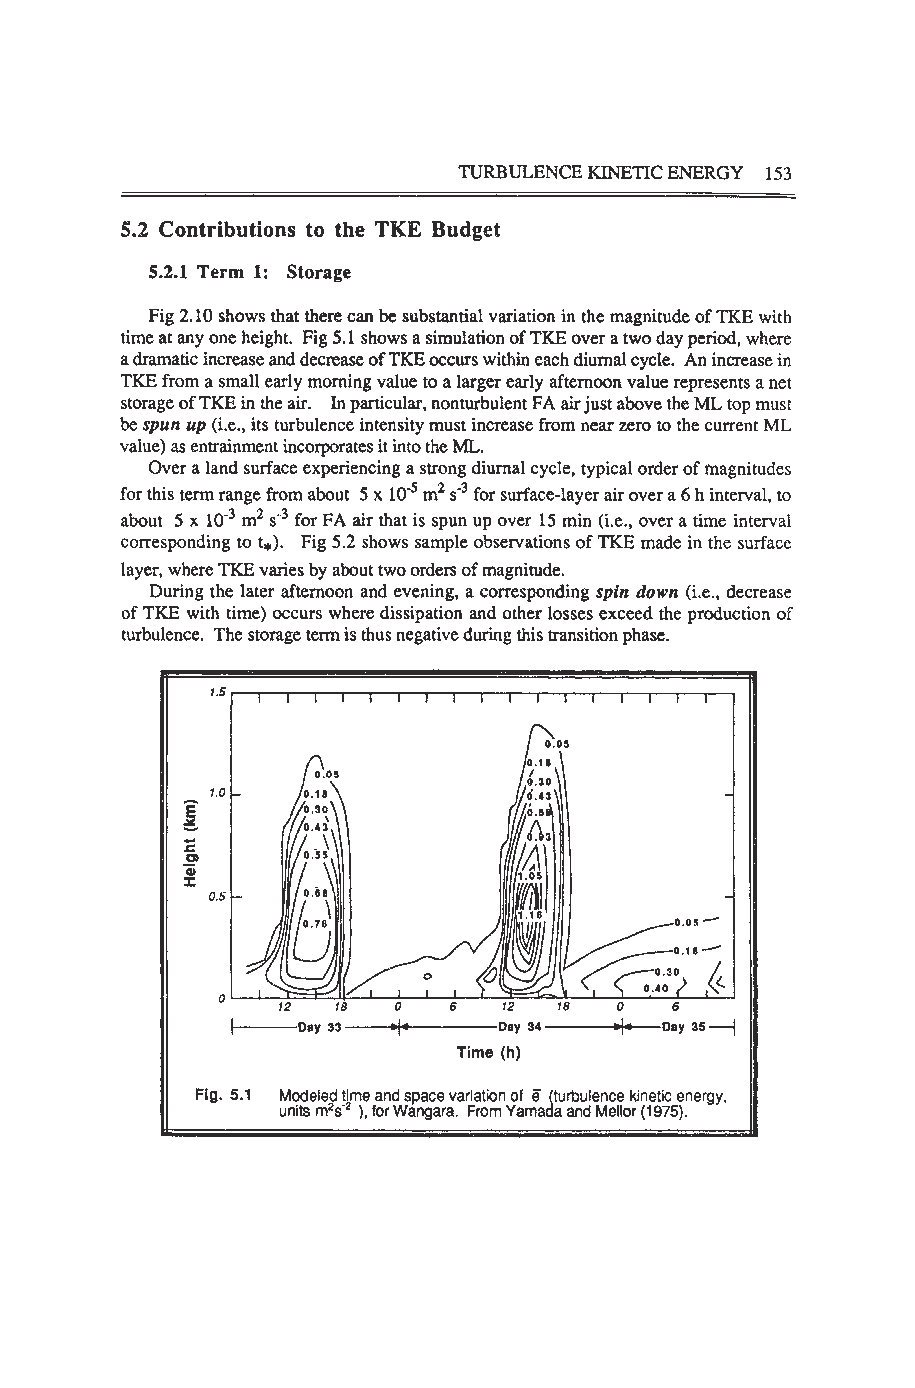
\includegraphics[width=0.9\linewidth,trim={3cm 5.5cm 2.9cm 11.6cm},clip]{fig/03/tke3}
%		\caption{Variación espacial y temporal de TKE modelada. Fuente: Stull (1988).}
%		\label{fig:03_tke3}
%	\end{figure}
%\end{frame}

\begin{frame}{Marco Teórico}{Simulación de Grandes Vórtices}
	Permite filtrar las pequeñas escalas de las grandes escalas a través de un operador de filtro:
	\begin{equation}
	\overline{u}(x_i,t) = \int G(r_i,x_j) u(x_j-r_i,t)dr_i
	\end{equation}
	Definimos una magnitud residual de la forma:
	\begin{equation}
	u' = u - \overline{u}.
	\end{equation}
\end{frame}

\begin{frame}{Marco Teórico}{Simulación de Grandes Vórtices}
	\begin{figure}[h!]
		\centering
		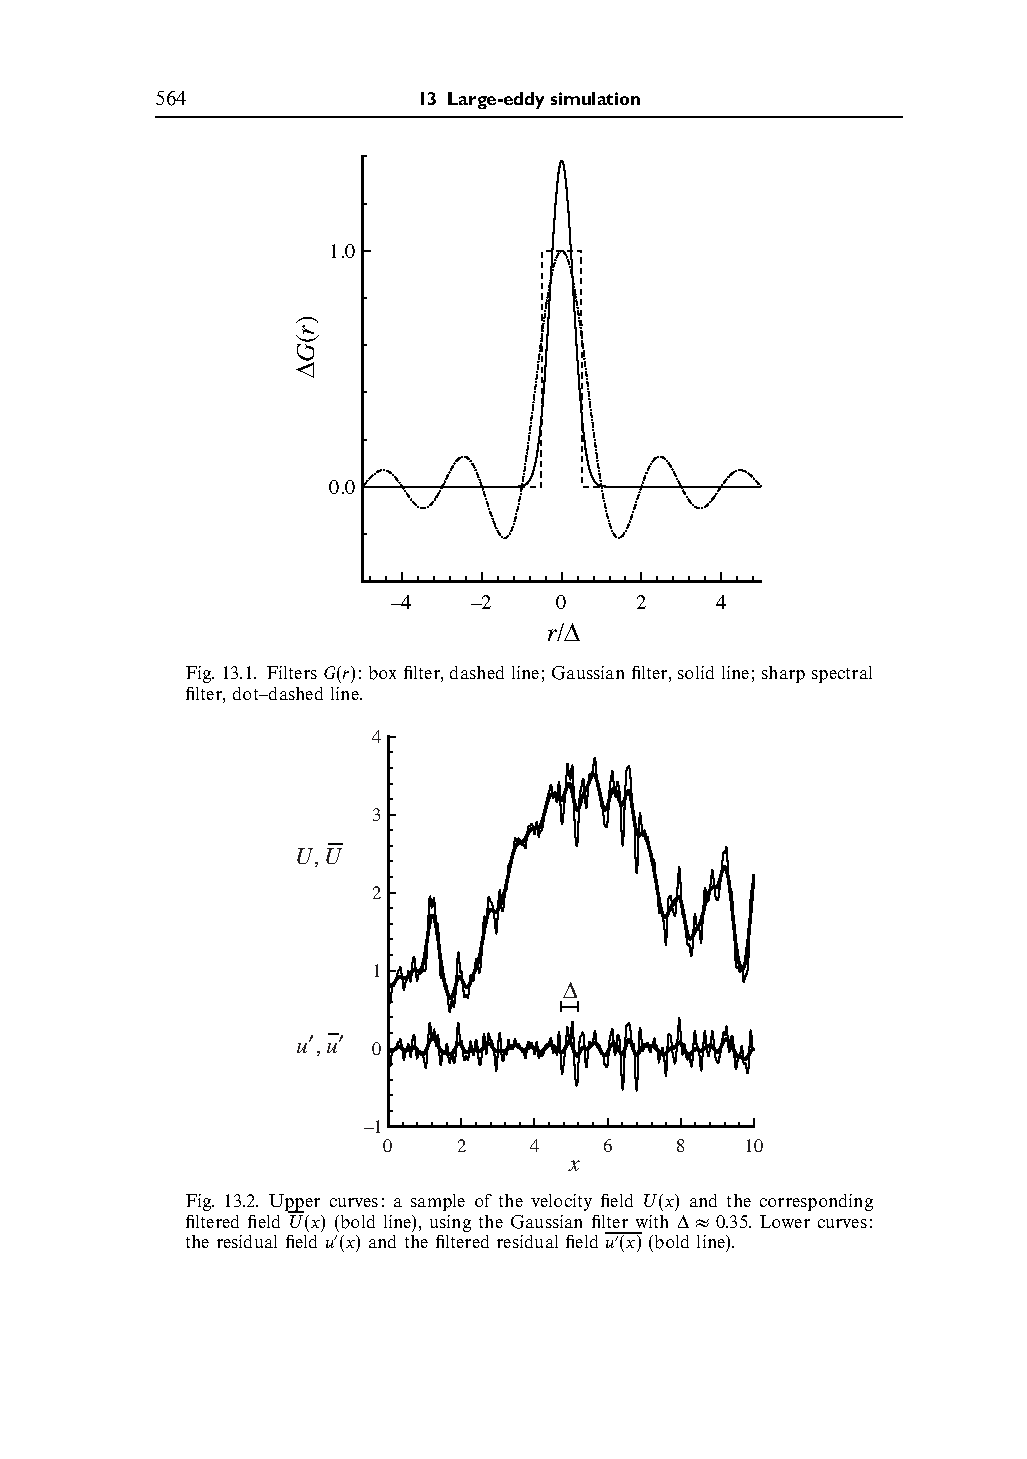
\includegraphics[width=0.7\linewidth,trim={4.8cm 4.8cm 2.8cm 12.1cm},clip]{fig/03/les}
		\caption{Curva superior: una muestra de un campo de velocidad $u$ y su correspondiente campo filtrado $\overline{u}$ (en negrita). Curva inferior: campo residual $u'$ y campo residual filtrado $\overline{u'}$ (en negrita). Fuente: Pope (2000).}
		\label{fig:03_les}
	\end{figure}
\end{frame}

\begin{frame}{Marco Teórico}{Simulación de Grandes Vórtices}
	Aplicando el filtro a las ecuaciones de N-S se obtiene el esfuerzo residual:
	\be \tau_{ij}^R \equiv \overline{u_j u_i} - \overline{u}_j \overline{u}_i \ee
	y su esfuerzo anisotrópico asociado es:
	\be \tau_{ij}^r = \tau_{ij}^R - \frac{2}{3}k_r \delta_{ij} \ee
	Este último se debe modelar.
\end{frame}

\begin{frame}{Marco Teórico}{Simulación de Grandes Vórtices}
	El esfuerzo $\tau_{ij}^r$ se puede modelar de diversas formas. Para esta tesis se modela utilizando el modelo 1.5TKE de Deardorff (1974):
	\begin{itemize}
		\item Se plantea una ecuación de transporte para la TKE residual $k_r$.
		\item La disipación se modela a través de:
		\be \varepsilon_r = \frac{C_E k_r^{3/2}}{\Delta} \ee
		\item Es esfuerzo se computa a través de una viscosidad turbulenta de la forma:
		\be \tau_{ij}^r = -2\nu_t \overline{S}_{ij} \ee
		\be \nu_t = C_\nu k_r^{1/2}\Delta \ee
	\end{itemize}
\end{frame}

\begin{frame}{Marco Teórico}{Asimilación de Datos}
	\textbf{Objetivo}: Hallar la mejor estimación del estado de la atmósfera combinando observaciones y resultados de un modelo.
	\begin{itemize}
		\item $x_a:$ Análisis (resultado del DA).
		\item $x_b:$ Background (del modelo numérico).
		\item $y:$ Observaciones (de la instrumentación).
	\end{itemize}
	De manera general se tiene:
	\begin{equation}
	\textbf{x}_a = \textbf{x}_b + \delta \textbf{x}
	\end{equation}
	\begin{equation}\label{eq:03_dataassim1}
	\textbf{x}_a = \textbf{x}_b + \textbf{K}(\textbf{y} - H(\textbf{x}_b))
	\end{equation}
	$\textbf{K}$ es la matriz de peso del proceso y $H(\textbf{x})$ es el operador de observación.
\end{frame}

\begin{frame}{Marco Teórico}{Asimilación de Datos: Análisis Variacional Tridimensional}
	En la práctica, el análisis se encuentra minimizando una función de costo:
	\be \small
	J(x) = J_b + J_o = \frac{1}{2}(\textbf{x}-\textbf{x}_b)^T \textbf{B}^{-1}(\textbf{x}-\textbf{x}_b) + \frac{1}{2}(H(\textbf{x})-\textbf{y})^T \textbf{R}^{-1}(H(\textbf{x})-\textbf{y})
	\ee
	De manera referencial, la solución se escribe:
	\be 
	\nabla J(x) = \textbf{B}^{-1}(\textbf{x}-\textbf{x}_b)-H^T\textbf{R}^{-1}(\textbf{y}-H(\textbf{x}))=0
	\ee
	El análisis es entonces:
	\be \label{eq:03_dataassim}
	\textbf{x}_a = \textbf{x}_b + \textbf{B}H^T(H\textbf{B}H^T+\textbf{R})^{-1}(\textbf{y}-H(\textbf{x}_b))
	\ee
	Como esto es costoso, la minimización se hace a través de un método numérico como un método de Newton o el gradiente conjugado.
\end{frame}






%WRF
\section{5. Modelo WRF}
\begin{frame}{Modelo WRF}{Aspectos Generales}
	El WRF-ARW es un modelo atmosférico de mesoescala no hidrostático que resuelve las ecuaciones de Euler para flujo compresible en su forma conservativa y utilizando una coordenada vertical de presión.
	
	Algunas características relevantes:
	\begin{itemize}
		\item Discretización espacial con malla escalonada, constante en la horizontal y variable en la vertical.
		\item Discretización temporal a través de RK3.
		\item Un filtro separa las ondas de alta frecuencia de las de baja frecuencia. Las ondas de alta frecuencia se integran en un paso de tiempo intermedio para asegurar estabilidad.
		\item Condiciones de borde reales e ideales.
		\item Anidamiento de dominios.
		\item Opciones de advección de hasta 6to orden.
		\item Físicas incluidas: Capa superficial, CLP, radiación, microfísicas y cúmulos.
	
	\end{itemize}
\end{frame}

\begin{frame}{Modelo WRF}{Coordenada Vertical}
	\begin{figure}[h!]
		\begin{minipage}{0.55\linewidth}
			\centering
			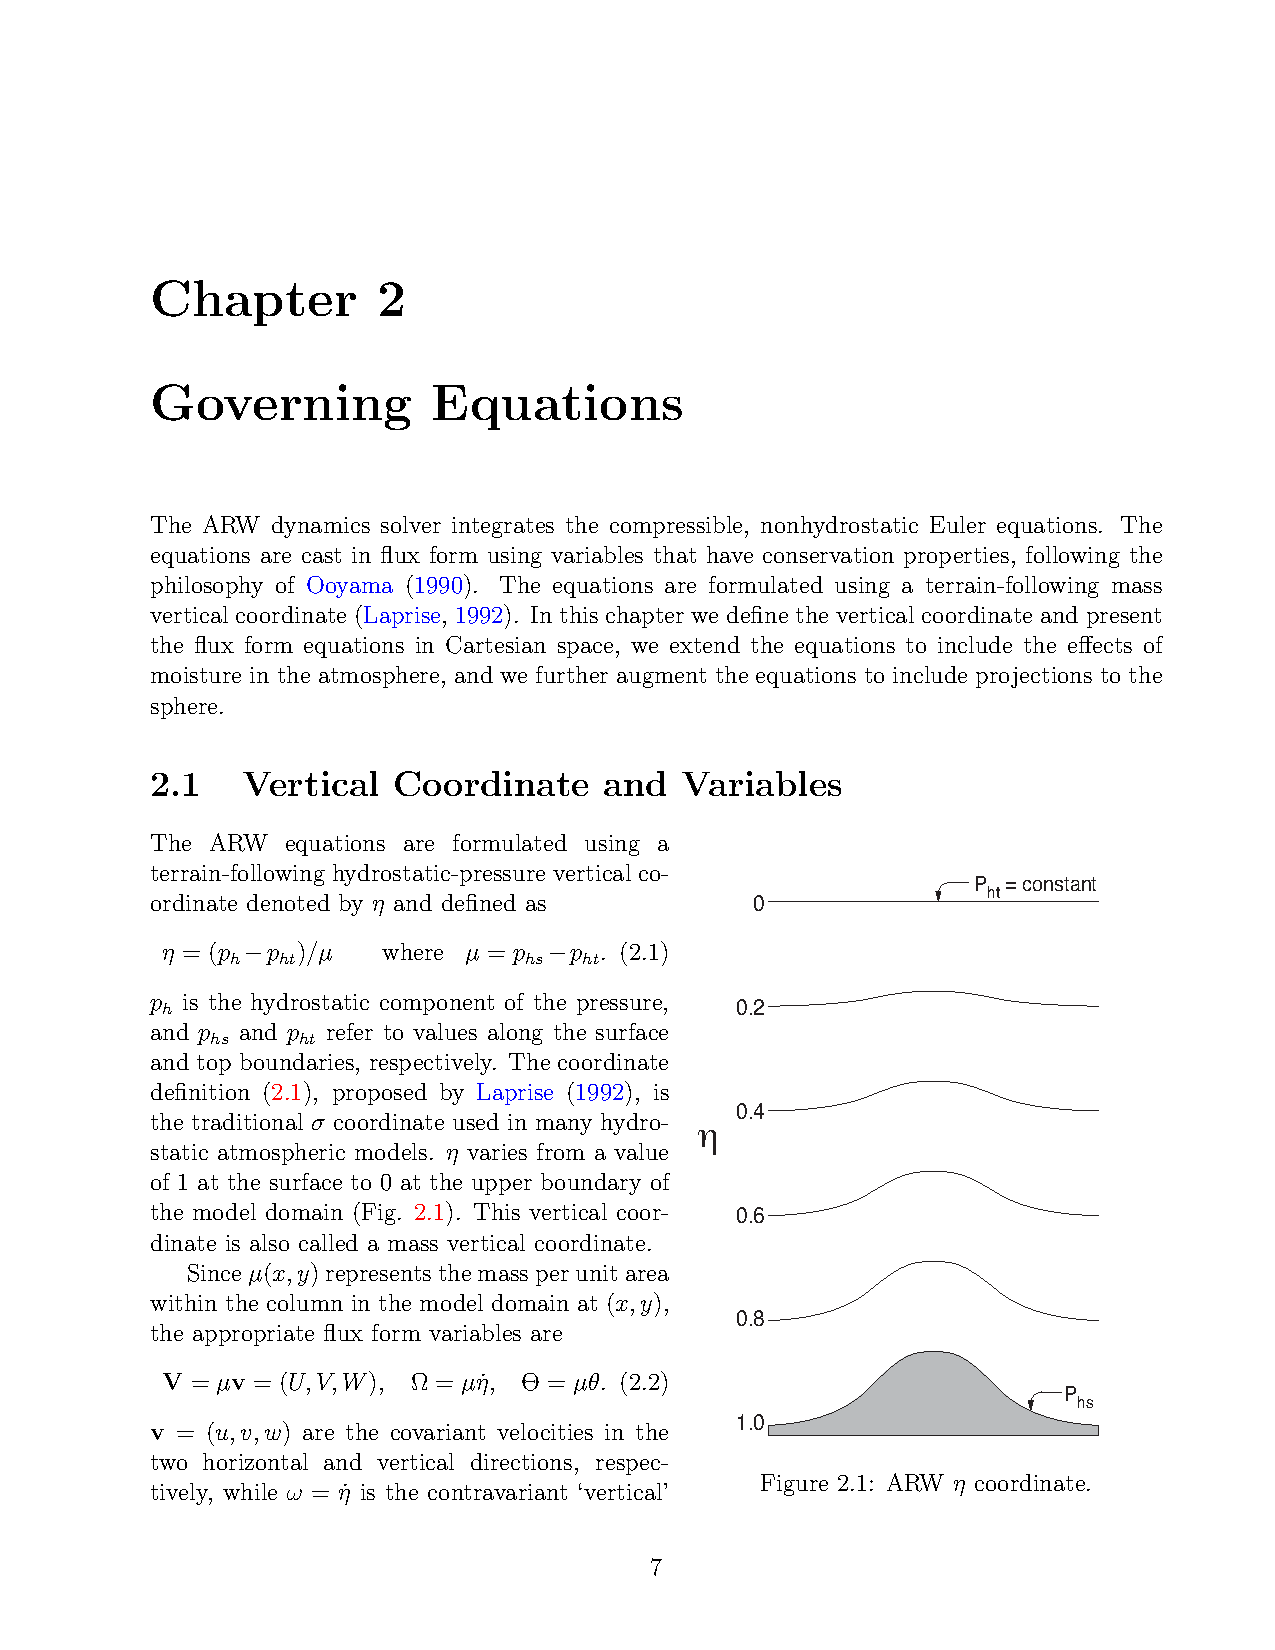
\includegraphics[width=0.95\linewidth,trim={11.5cm 3.3cm 1cm 14cm},clip]{fig/04/eta}
			\caption{Estructura de la coordenada vertical. Fuente: Shamarock et al. (2008).}
			\label{fig:04_eta}
		\end{minipage}%
		\begin{minipage}{0.45\linewidth}
			Se define $\eta$ como:
			\[ \eta = \frac{p_{dh}-p_{dht}}{\mu_d} = \frac{p_{dh}-p_{dht}}{p_{dhs}-p_{dht}} \]
			$\mu_d:$ Peso de la columna de aire.
			
			\bigskip
			\bigskip
			
			El modelo resuelve:\\
			\[(u,v,w,\mu_d,\phi, \theta,p,\alpha,k)\]
		\end{minipage}%
	\end{figure}
\end{frame}

\begin{frame}{Modelo WRF}{Ecuaciones Resueltas}
	\small
	\begin{equation}\begin{split}\label{eq:04_wrf1}
	&\partial_t U + m_x[\partial_x(Uu)+\partial_y(Vu)]+\partial_\eta(\Omega u) \\
	&+ (m_x/m_y)(\alpha/\alpha_d)[\mu_d(\partial_x\phi' + \alpha_d \partial_x p' + \alpha_d'\partial_x \overline p)+\partial_x\phi(\partial_\eta p' - \mu_d')] = F_U
	\end{split}\end{equation}
	\begin{equation}\begin{split}
	&\partial_t V + m_y[\partial_x(Uv)+\partial_y(Vv)]+(m_y/m_x)\partial_\eta(\Omega v) \\
	&+ (m_y/m_x)(\alpha/\alpha_d)[\mu_d(\partial_y\phi' + \alpha_d \partial_y p' + \alpha_d'\partial_y \overline p)+\partial_y\phi(\partial_\eta p' - \mu_d')] = F_V
	\end{split}\end{equation}
	\begin{equation}\begin{split}
	\partial_t W + m_x[\partial_x(&Uw)+\partial_y(Vw)]+\partial_\eta(\Omega w) \\
	\hspace{1cm}&- m_y^{-1}g(\alpha/\alpha_d)[\partial_\eta p' - \overline{\mu}_d(q_v+q_c+q_r)]+m_y^{-1}\mu_d' g = F_W
	\end{split}\end{equation}
	\begin{equation}\begin{split}
	\partial_t \mu_d' + m_x m_y[\partial_x U + \partial_y V] + m_y\partial_\eta \Omega = 0
	\end{split}\end{equation}
	\begin{equation}\begin{split}
	\partial_t \phi' + \mu_d^{-1}[m_x m_y(U\partial_x\phi + V\partial_y\phi) + m_y \Omega \partial_\eta\phi - m_ygW] = 0
	\end{split}\end{equation}
	\begin{equation}\begin{split}\label{eq:04_wrf2}
	\partial_t \Theta + m_x m_y [\partial_x(U\theta)+\partial_y(V\theta)]+m_y\partial_\eta(\Omega \theta) = F_\Theta
	\end{split}\end{equation}
\end{frame}


\begin{frame}{Modelo WRF}{Modelación de la Turbulencia}
	Dentro del modelo el tensor de esfuerzos turbulentos es:
	\be \tau_{ij}=-\mu_d K_{h,v}S_{ij} \ee
	La manera de computar $K_{h,v}$ va a depender de la escala espacial en la que estemos (parametrización/LES).
	\bigskip
	
	Para la mesoescala:
	\begin{align}
	K_h &= C_s^2 l^2[0.25(S_{11}-S_{22})^2+S_{12}]^{0.5}\\
	K_v &= f(PBL)
	\end{align}
\end{frame}

\begin{frame}{Modelo WRF}{Modelación de la Turbulencia}
	
	Para la microescala (LES):
	\begin{equation}K_{h,v}=C_k l_{h,v}\sqrt{k}.\end{equation}
	$C_k$ es la constante del modelo y $l_{h,v}$ es un largo característico.
	
	La ecuación de transporte para $k$:
	\begin{equation}
	\partial_t(\mu_d k) + (\nabla\cdot\vec{V}k)_\eta = \mu_d(\mathcal{P} + \mathcal{F} + \mathcal{D}).
	\end{equation}
	El RHS corresponde a la producción mecánica, producción por flotación y disipación de $k$.
	\begin{align}
	\mathcal{P}&= K_h (S_{11}^2 + S_{22}^2 + S_{12}^2) + K_v (S_{33}^2 + S_{13}^2 + S_{23}^2),\\
	\mathcal{F}&=-K_v N^2,\\
	\mathcal{D}&=-\frac{C k^{3/2}}{l_k},
	\end{align}
\end{frame}






%METODOLOGIA
\section{6. Metodología}
\begin{frame}{Metodología}
	\begin{figure}[h!]
		\centering
		%\vspace{0.2cm}
		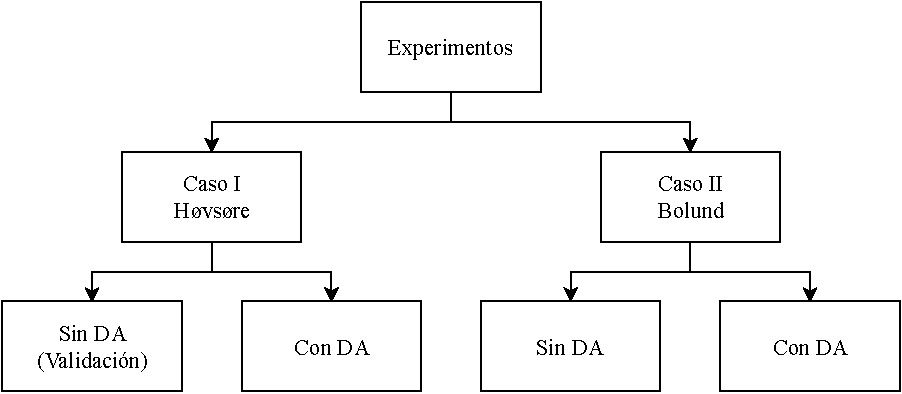
\includegraphics[width=1\linewidth,clip]{tesis_experimentos}%
		\caption{Diagrama de experimentos realizados.}
	\end{figure}
\end{frame}
%HOVSORE
\begin{frame}{Metodología}{Selección de Dominios: Caso I Høvsøre}
	 \begin{figure}[H]
	 	\centering\frame{
	 		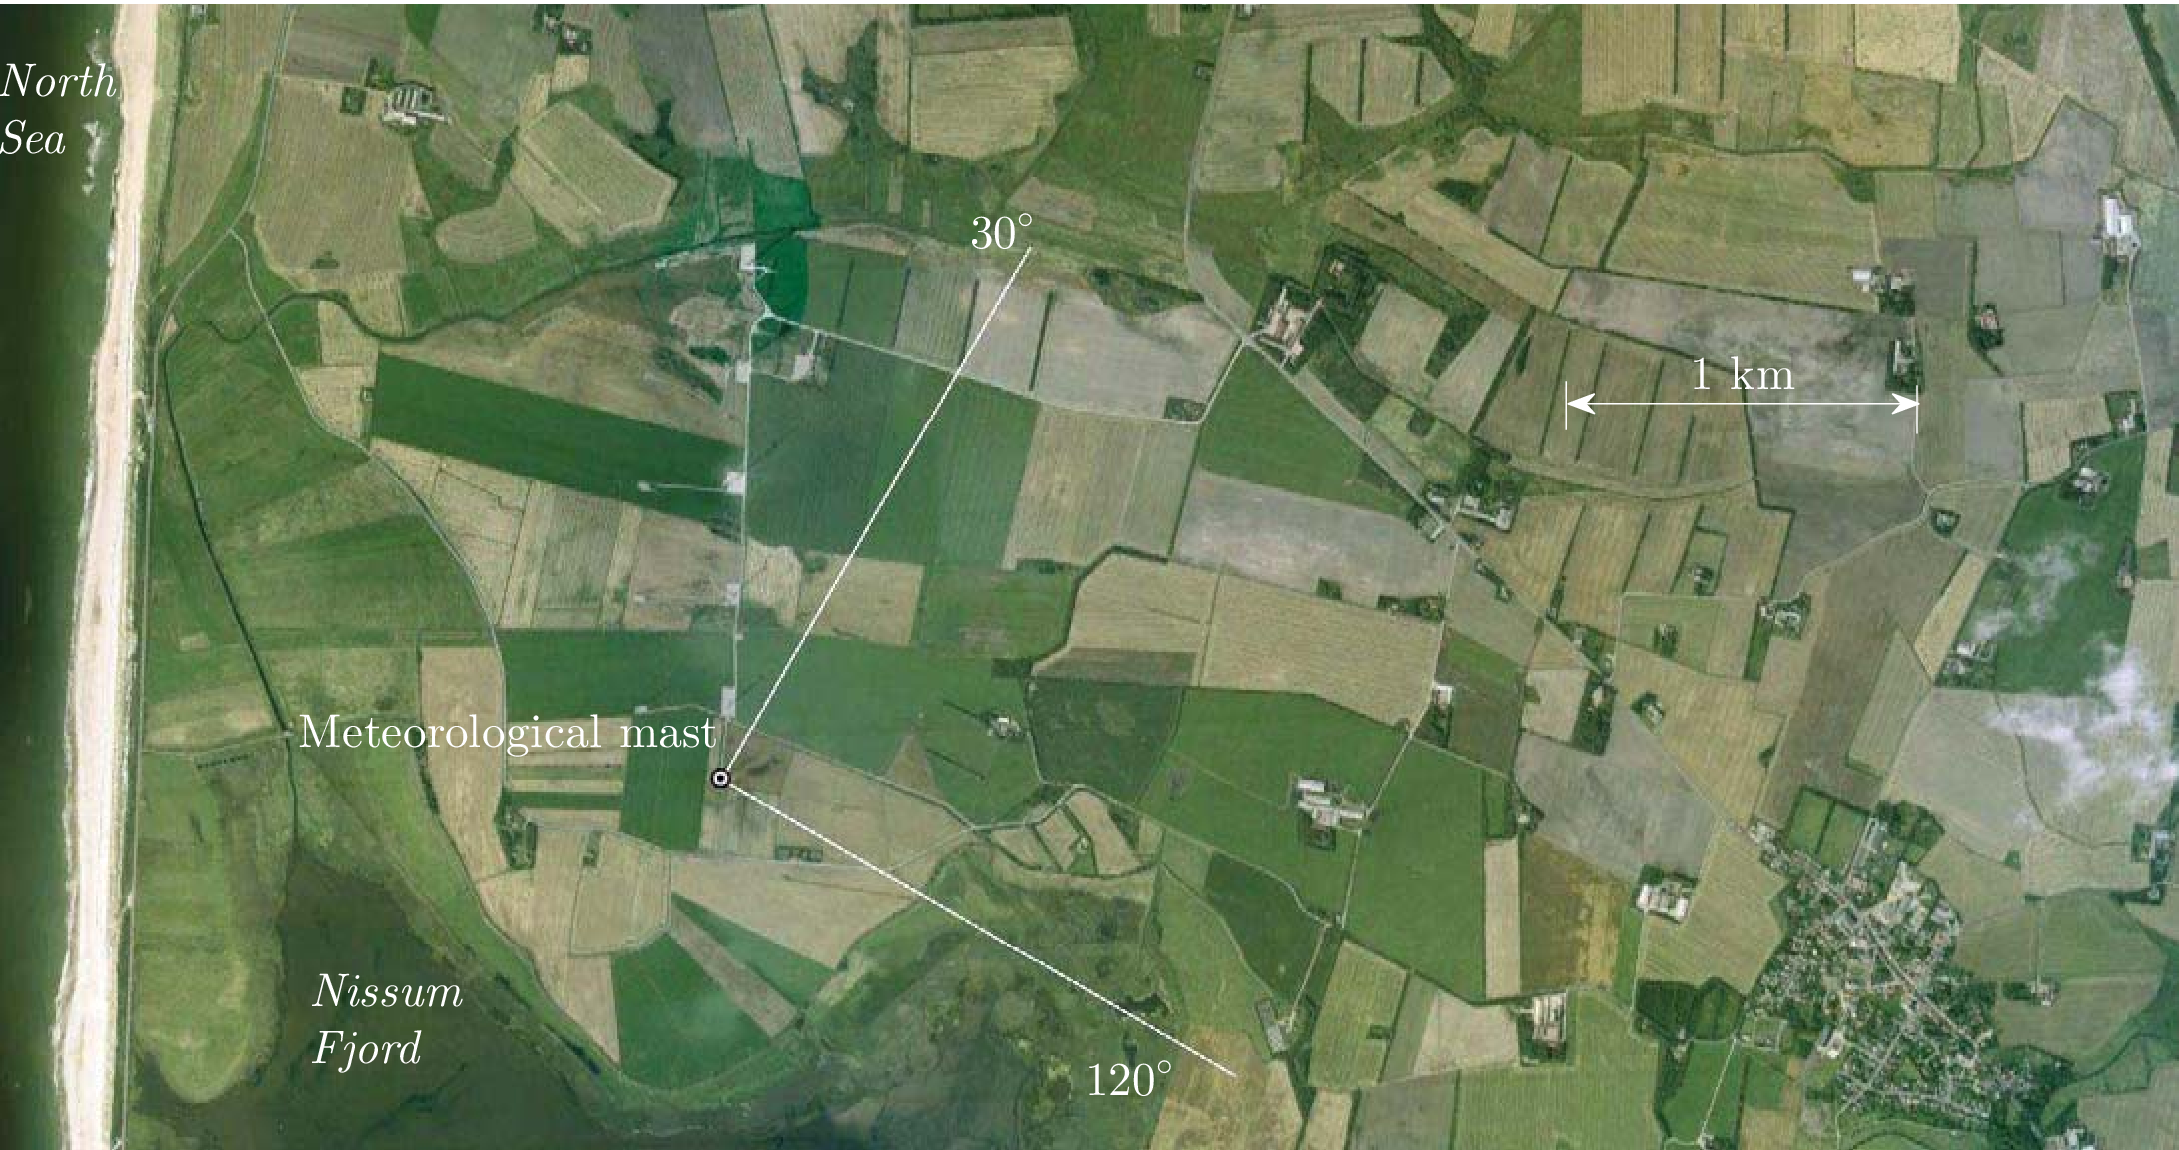
\includegraphics[width=0.98\linewidth,page=1,trim={0cm 0cm 0cm 0cm},clip]{fig/05/hovsore}}%
	 	\caption{Fotografía del terreno en Høvsøre. Fuente: Peña et al.(2013)}
	 	\label{fig:05_terreno_hovsore}
	 \end{figure}
\end{frame}

\begin{frame}{Metodología}{Configuración: Caso I Høvsøre}
	\begin{figure}[H]
		\centering
		\begin{minipage}{0.5\linewidth}
			\center(a)
		\end{minipage}%
		\begin{minipage}{0.5\linewidth}
			\center(b)
		\end{minipage}%
		
		\frame{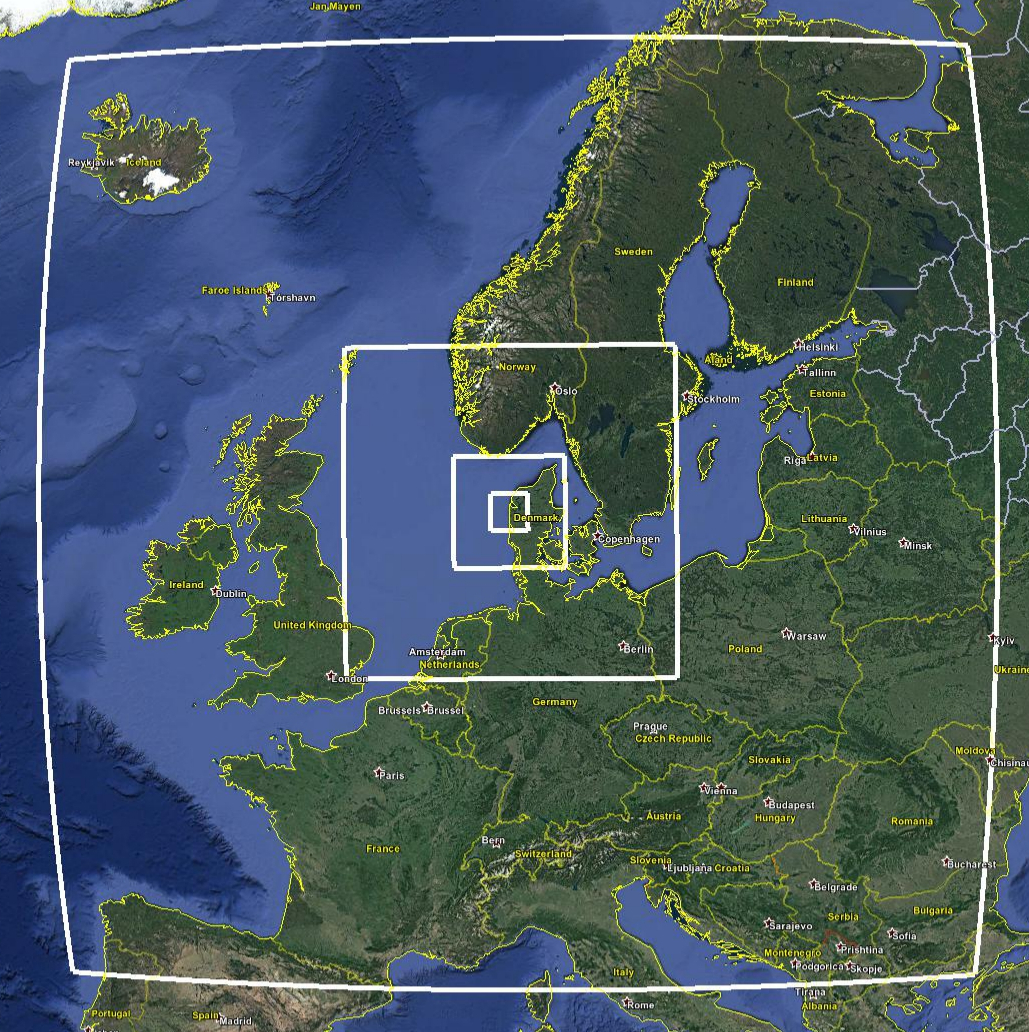
\includegraphics[width=0.45\linewidth,trim={0cm 0cm -0cm 0cm},clip]{fig/05/hov_dom1_edit.jpg}}\hspace{0.5cm}%
		\frame{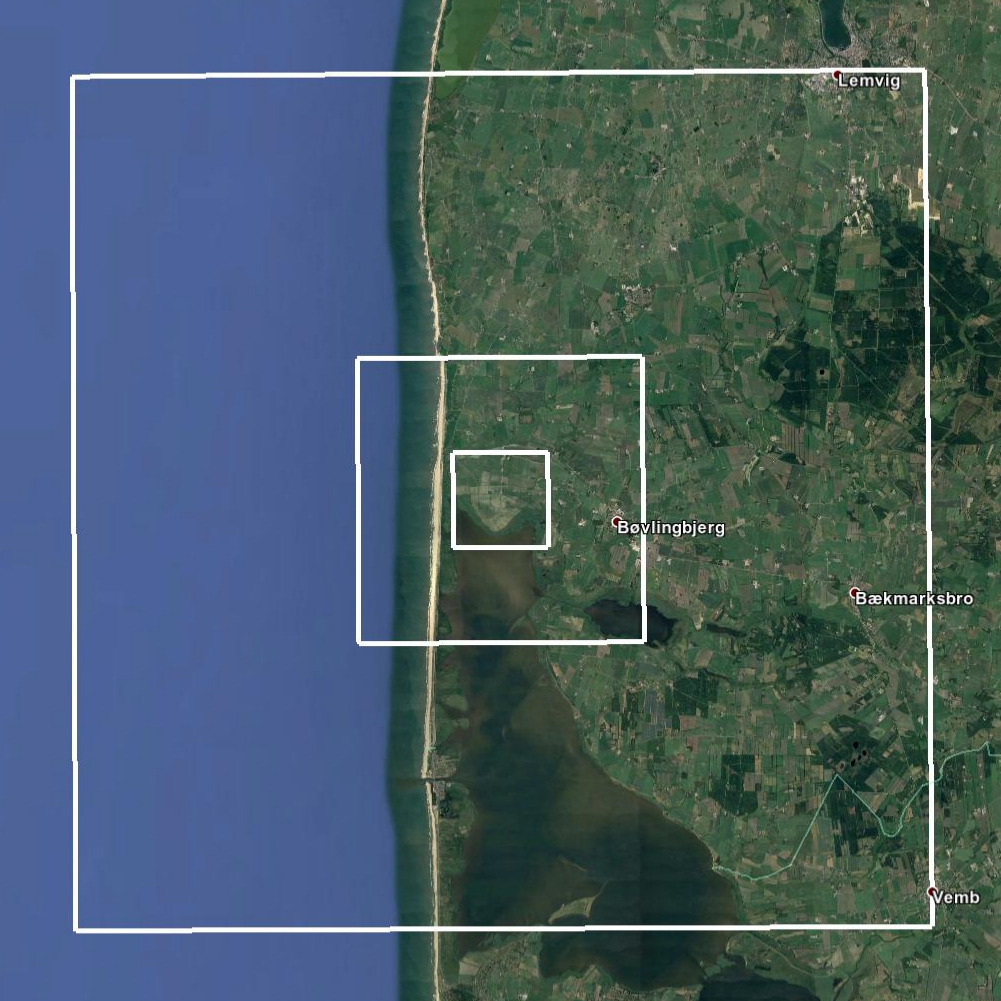
\includegraphics[width=0.45\linewidth,trim={0cm 0cm 0cm 0cm},clip]{fig/05/hov_dom2_edit.jpg}}\vspace{0.3cm}%
		
		\caption{Información de los dominios de simulación para el caso Høvsøre. (a) Dominios d01-d04. (b) Dominios d05-d07.}
		\label{fig:05_dom_hov_a}
	\end{figure}
\end{frame}

\begin{frame}{Metodología}{Configuración: Caso I Høvsøre}
	\begin{figure}[H]
		\centering
		\begin{minipage}{0.5\linewidth}
			\center \hspace{1.5cm}(c)
		\end{minipage}%
		\begin{minipage}{0.5\linewidth}
			\center(d)
		\end{minipage}%
		
		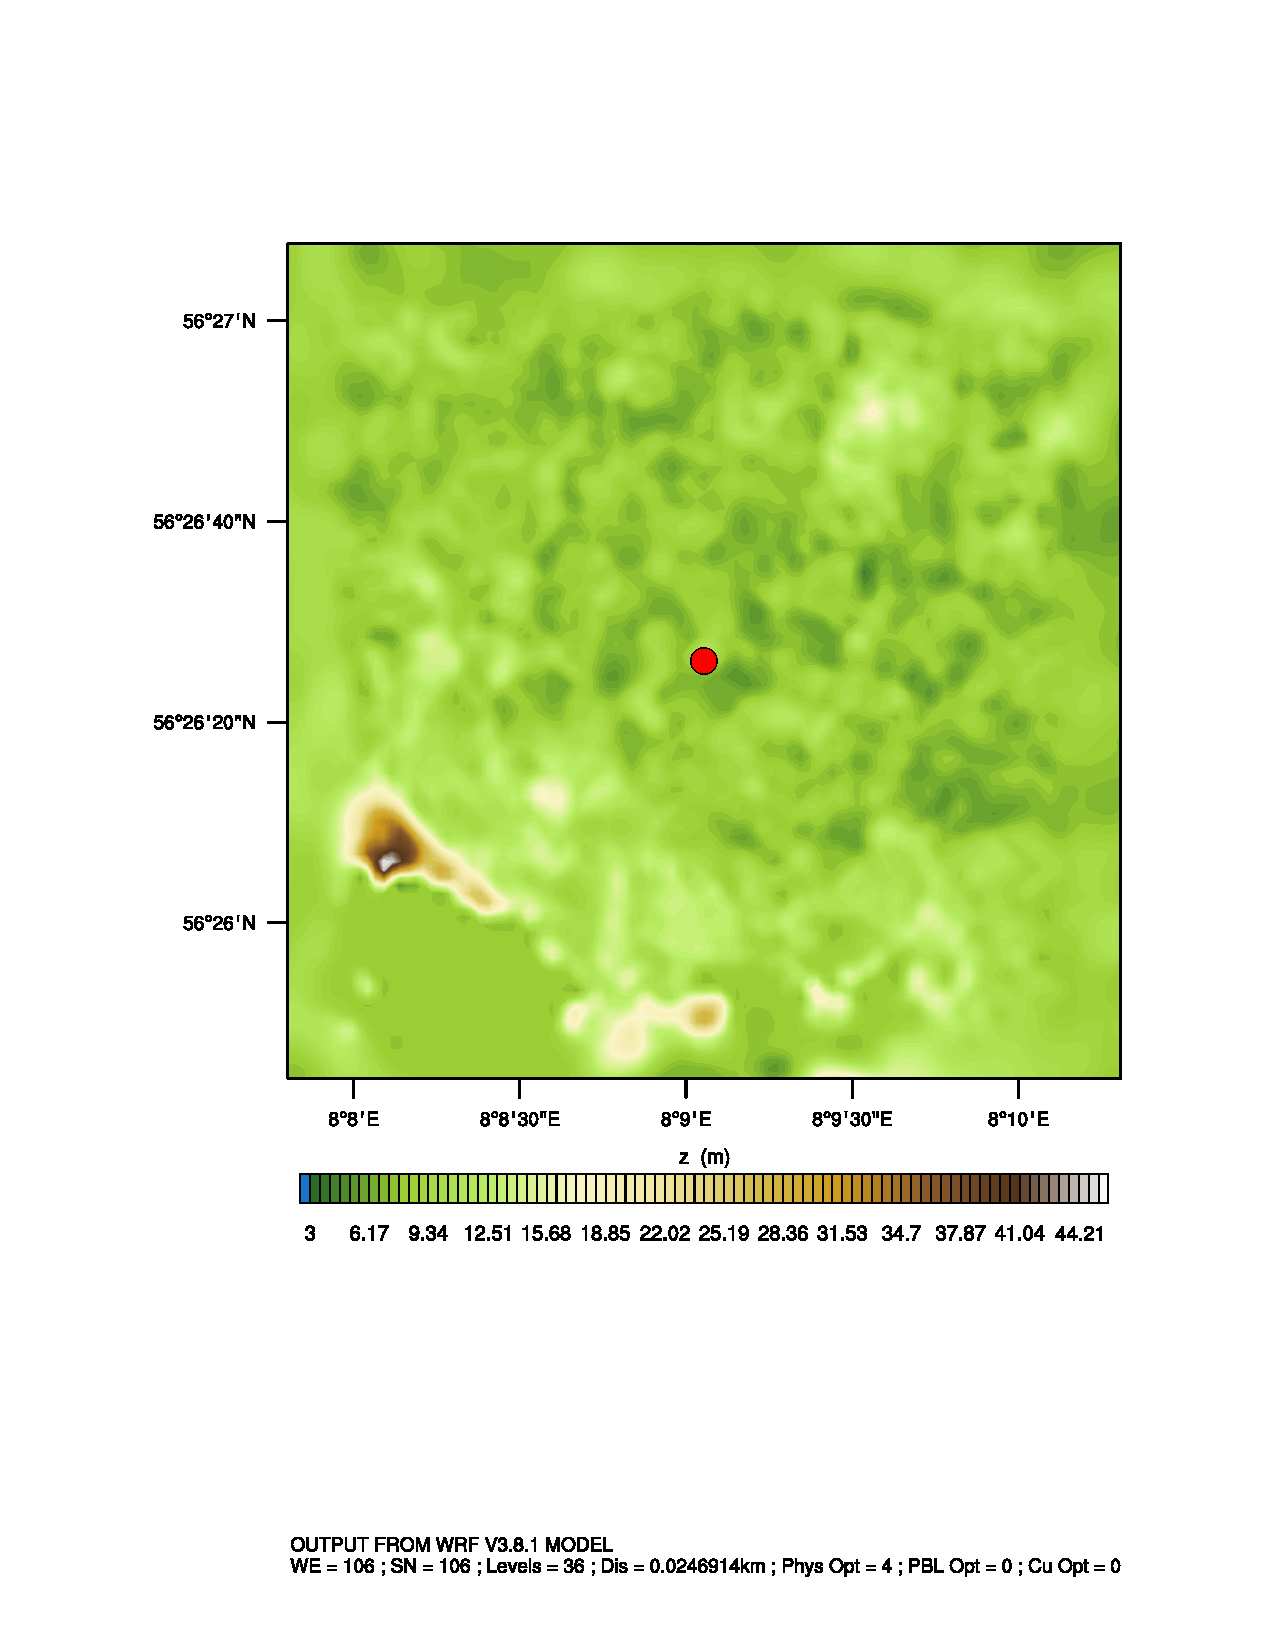
\includegraphics[width=0.45\linewidth,trim={2.5cm 6.5cm 2cm 3.5cm},clip]{fig/05/hov_control_point.pdf}%
		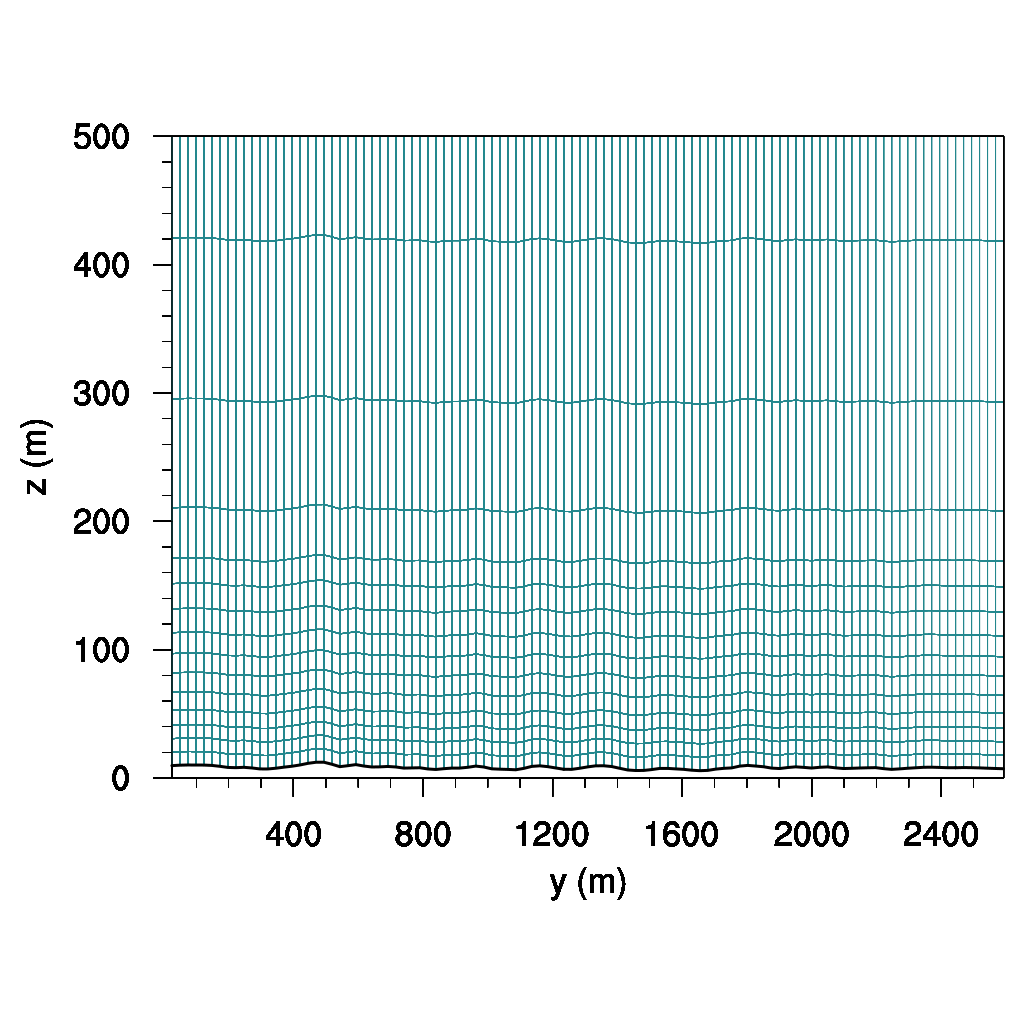
\includegraphics[width=0.45\linewidth,trim={0.5cm 0cm 0cm -1.3cm},clip]{fig/05/mesh57}%
		
		\caption{Información de los dominios de simulación para el caso Høvsøre. (c) Dominio d07 con el punto de control. (d) Distribución vertical de la malla adaptativa en escala 4:1.}
		\label{fig:05_dom_hov_b}
	\end{figure}
\end{frame}

\begin{frame}{Metodología}{Configuración: Caso I Høvsøre}
	\begin{table}[h!]
		\caption{Dominio numérico espacial y temporal para simulación del caso Høvsøre.}\label{tab:05_config_hov}
		\centering\footnotesize
		\begin{tabular}{lcc}
			\toprule
			Parámetro & Selección \\
			\midrule
			Fecha	 	 & 2010-09-08   \\
			Hora Inicio	 	 & 06:00:00   UTC \\
			Hora Término	 		 & 20:00:00 UTC  \\
			Puntos Malla Vert.	 	 & 37   \\
			$P_{top}$ 	& 30000 [Pa]\\
			\# Dominios	& 7   \\
			Lat. Centro	& 56.440588   \\
			Lon. Centro	& 8.150896   \\
			Interválo Salida & 10 [min]\\
			Punto de Malla Total & 2,831,472\\
			\bottomrule
		\end{tabular}
	\end{table}
\end{frame}

\begin{frame}{Metodología}{Configuración: Caso I Høvsøre}
	\vspace{-3mm}
	\begin{table}[h!]
	\caption{Valores característicos de cada dominio en Høvsøre.}\label{tab:05_caract_hov}
	\vspace{-4mm}
	\centering\scriptsize\resizebox{\textwidth}{!}{
		\begin{tabular}{lccccccc}
			\toprule
			Dominio 				& d01	&	d02	&	d03	&	d04	&	d05	&	d06 &	d07 \\
			\midrule
			$N_x$		& 107 & 107 & 107 &107&107&107&107  \\
			$N_y$	 		& 107 & 107 & 107 &107&107&107&107  \\
			$\Delta x, y$	[m]	 		& 30000 & 10000 & 3333.3 &1111.1&222.22&74.074&24.691  \\
			$\Delta t$	[s]	 		& 75 & 25 & 8.333 &2.778&0.556&0.185&0.062  \\
			Orografía		 	& GMTED & GMTED & GMTED &ASTER&ASTER&ASTER&ASTER  \\
			Uso de Suelo		& USGS & USGS & USGS &CLC12&CLC12&CLC12&CLC12 \\
			\bottomrule
		\end{tabular}}
	\end{table}
	\vspace{-3mm}
	\begin{table}[h!]
		\caption{Parametrizaciones físicas utilizadas en el modelo para Høvsøre.}\label{tab:05_param_hov}
		\vspace{-4mm}
		\centering\scriptsize\resizebox{\textwidth}{!}{
			\begin{tabular}{lccccccc}
				\toprule
				Dominio 				& d01	&	d02	&	d03	&	d04	&	d05	&	d06 &	d07 \\
				\midrule
				Micro-físicas		 	& WSM5 & WSM5 & WSM5 &WSM5&WSM5&WSM5&WSM5  \\
				Cúmulos			 		& Grell & Grell & -- & -- & -- & -- & -- \\ 
				Capa Superficial	 	& MYNN & MYNN & MYNN & MYNN & MYNN & MYNN & MYNN \\
				PBL				 		& MYNN & MYNN & MYNN & MYNN & -- & -- & -- \\
				Modelo LES				 		& -- & -- & -- & -- & 1.5TKE & 1.5TKE & 1.5TKE \\
				$c_k$				 		& -- & -- & -- & -- & 0.3 & 0.3 & 0.3 \\
				Modelo de Suelo 		& Difus. & Difus. & Difus. & Difus. & Difus. & Difus. & Difus. \\
				Rad. Onda Larga	& RRTM &RRTM&RRTM&RRTM&RRTM&RRTM&RRTM \\
				Rad. Onda Corta	& Dudhia &Dudhia&Dudhia&Dudhia&Dudhia&Dudhia&Dudhia \\
				\bottomrule
			\end{tabular}}
		\end{table}
\end{frame}

%BOLUND
\begin{frame}{Metodología}{Selección de Dominios: Caso II Bolund}
	\begin{figure}[H]
		\centering\frame{
			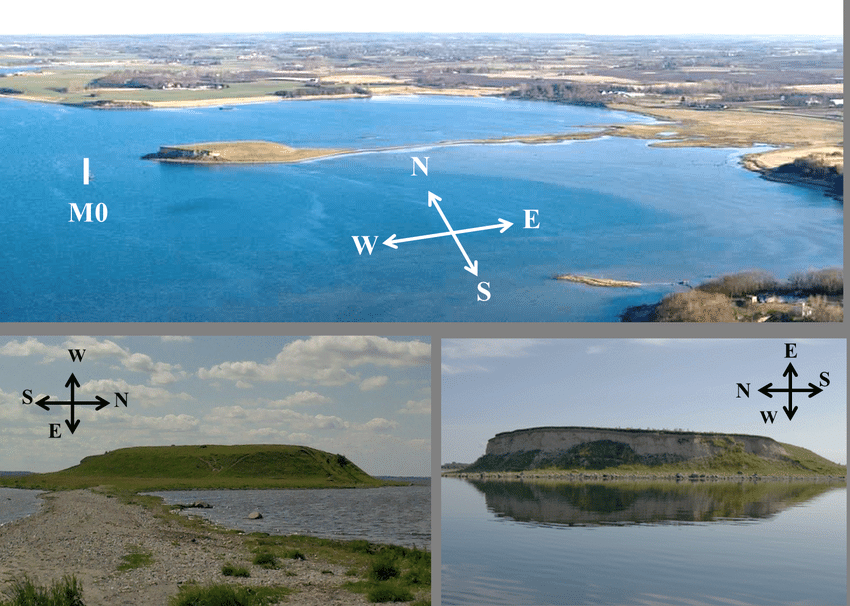
\includegraphics[width=0.8\linewidth,page=1,trim={0cm 0cm 0cm 0cm},clip]{fig/05/bolund}}%
		\caption{Fotografías de la colina de Bolund. Fuente: Chaudhari (2014)}
		\label{fig:05_terreno_bolund}
	\end{figure}
\end{frame}

\begin{frame}{Metodología}{Configuración: Caso II Bolund}
	\begin{figure}[H]
		\centering
		\frame{\includegraphics[width=0.48\linewidth,page=1,trim={5mm 3mm 3mm 3mm},clip]{fig/05/bol_d1-2-3-4edit.jpg}}
		\frame{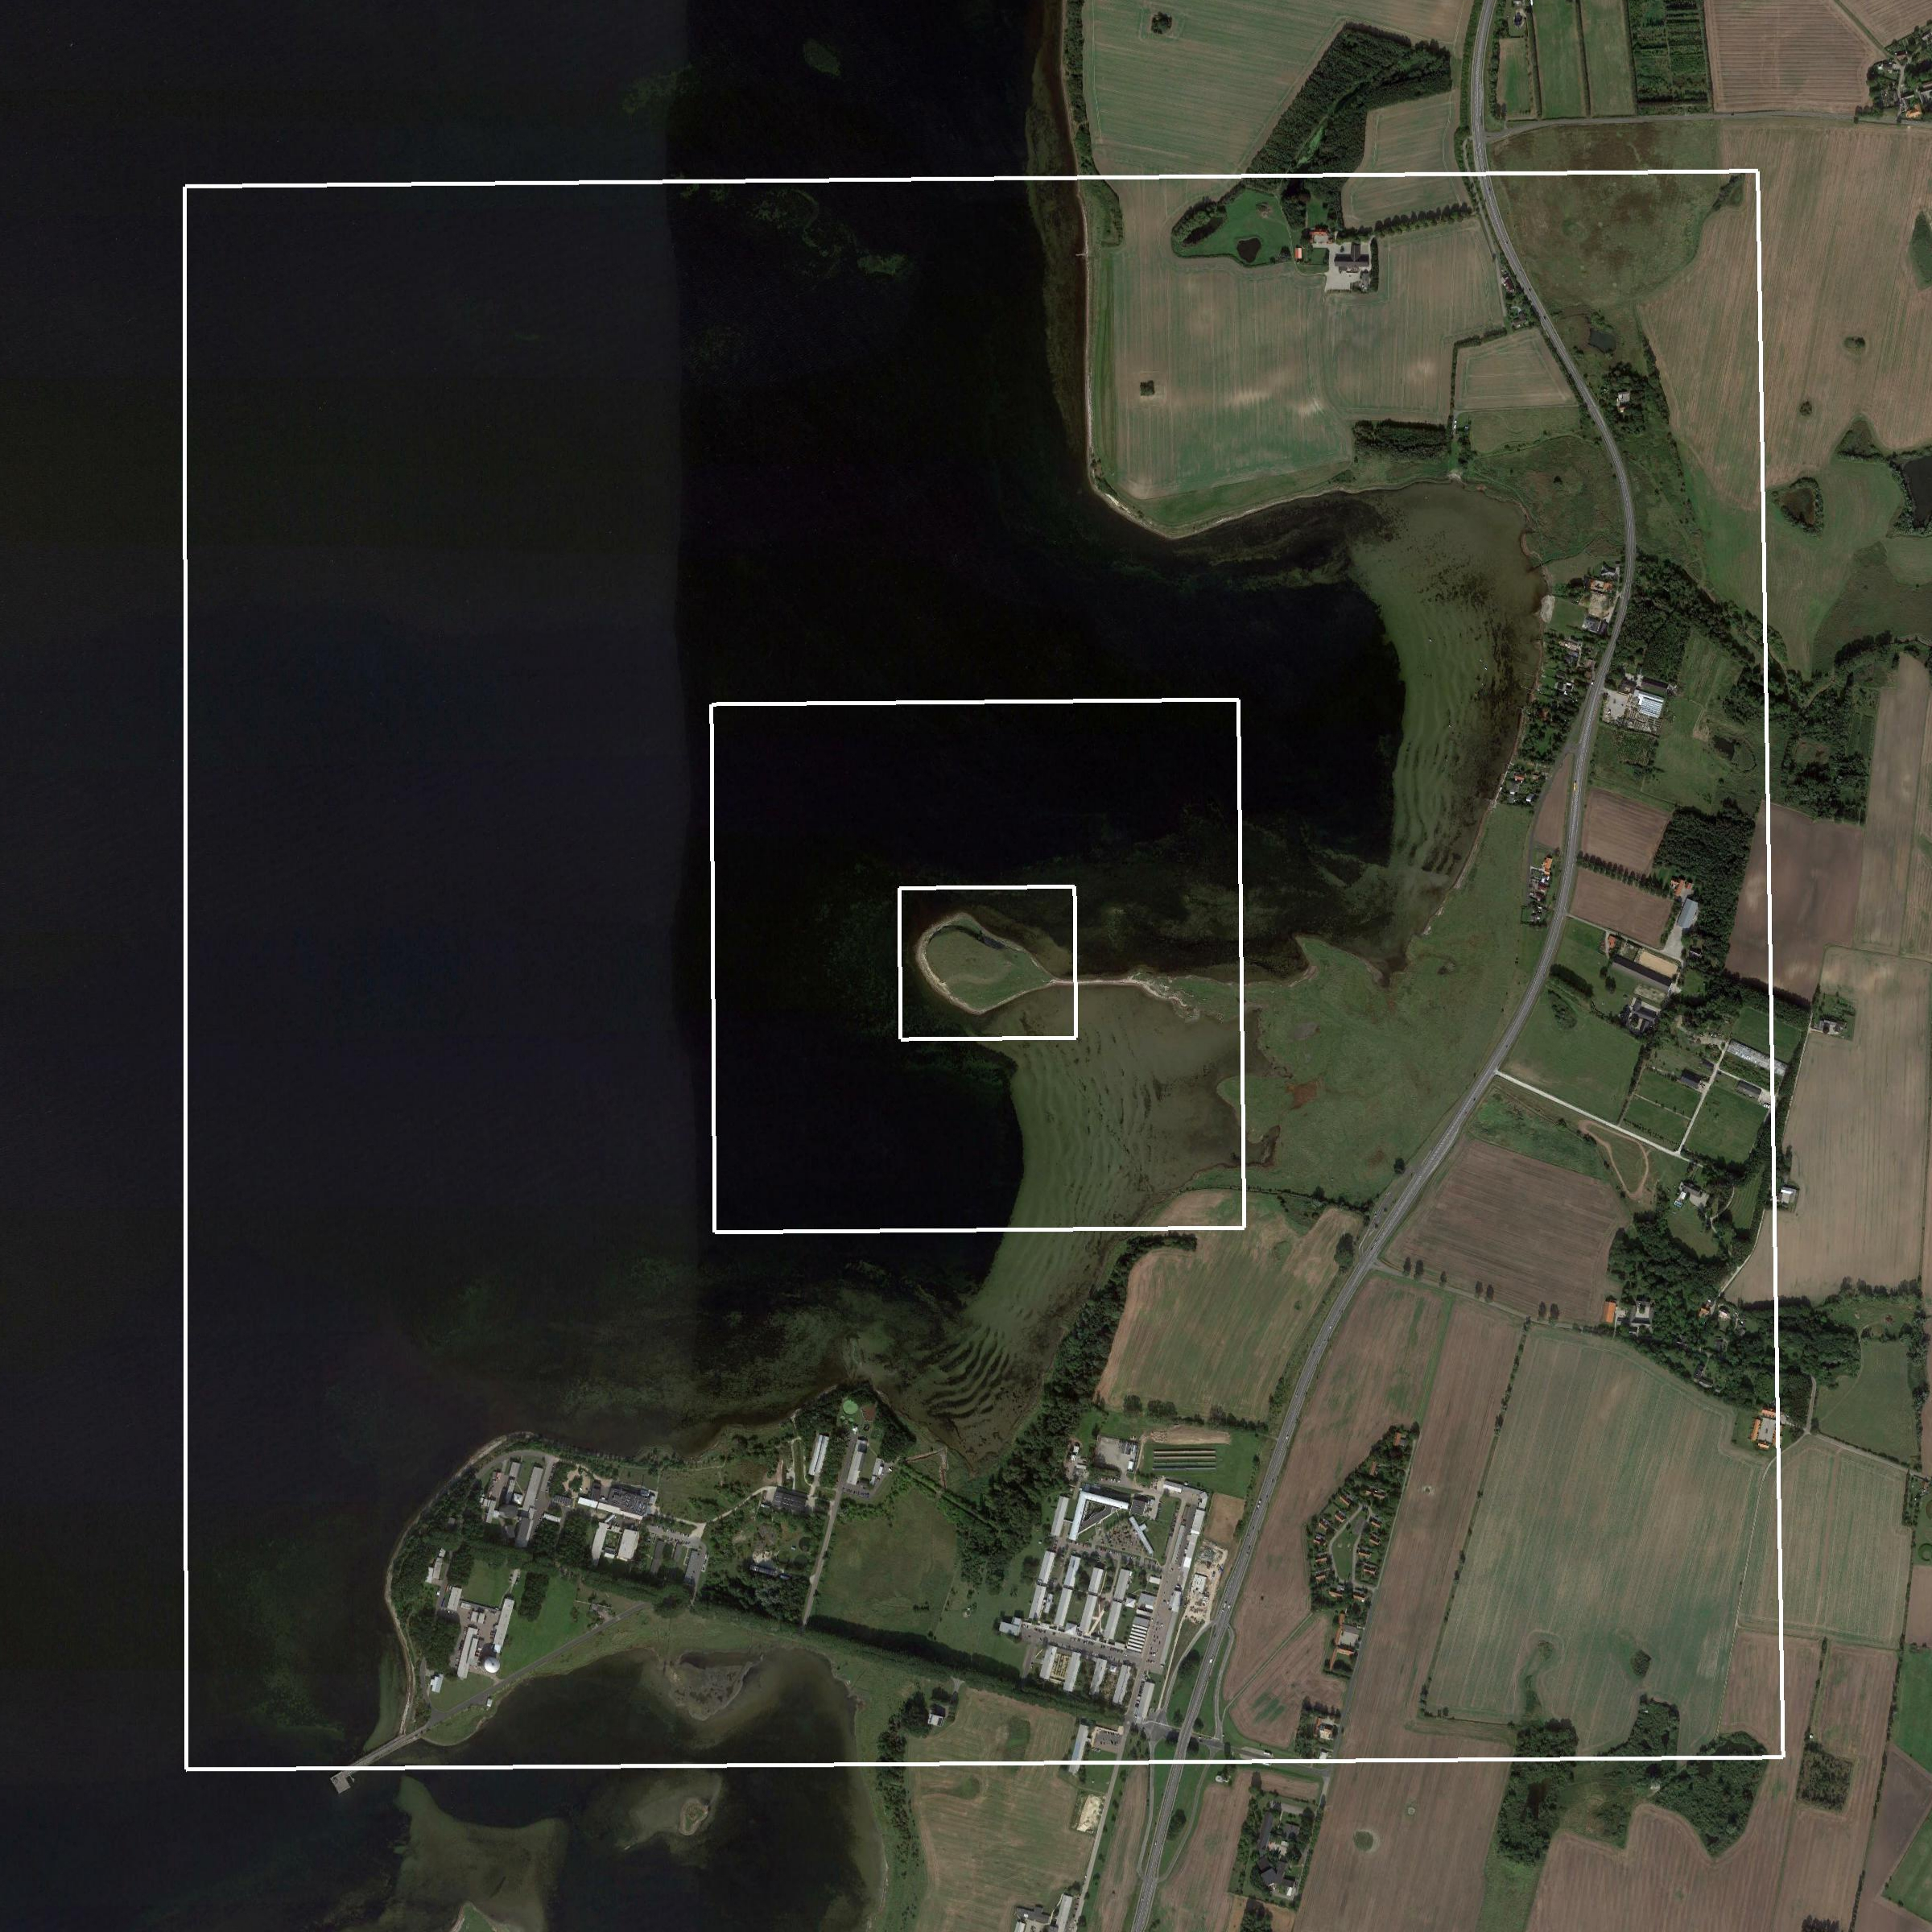
\includegraphics[width=0.48\linewidth,page=1,trim={5mm 3mm 3mm 3mm},clip]{fig/05/bol_d6-7-8edit.jpg}}
		
		%\bigskip
		%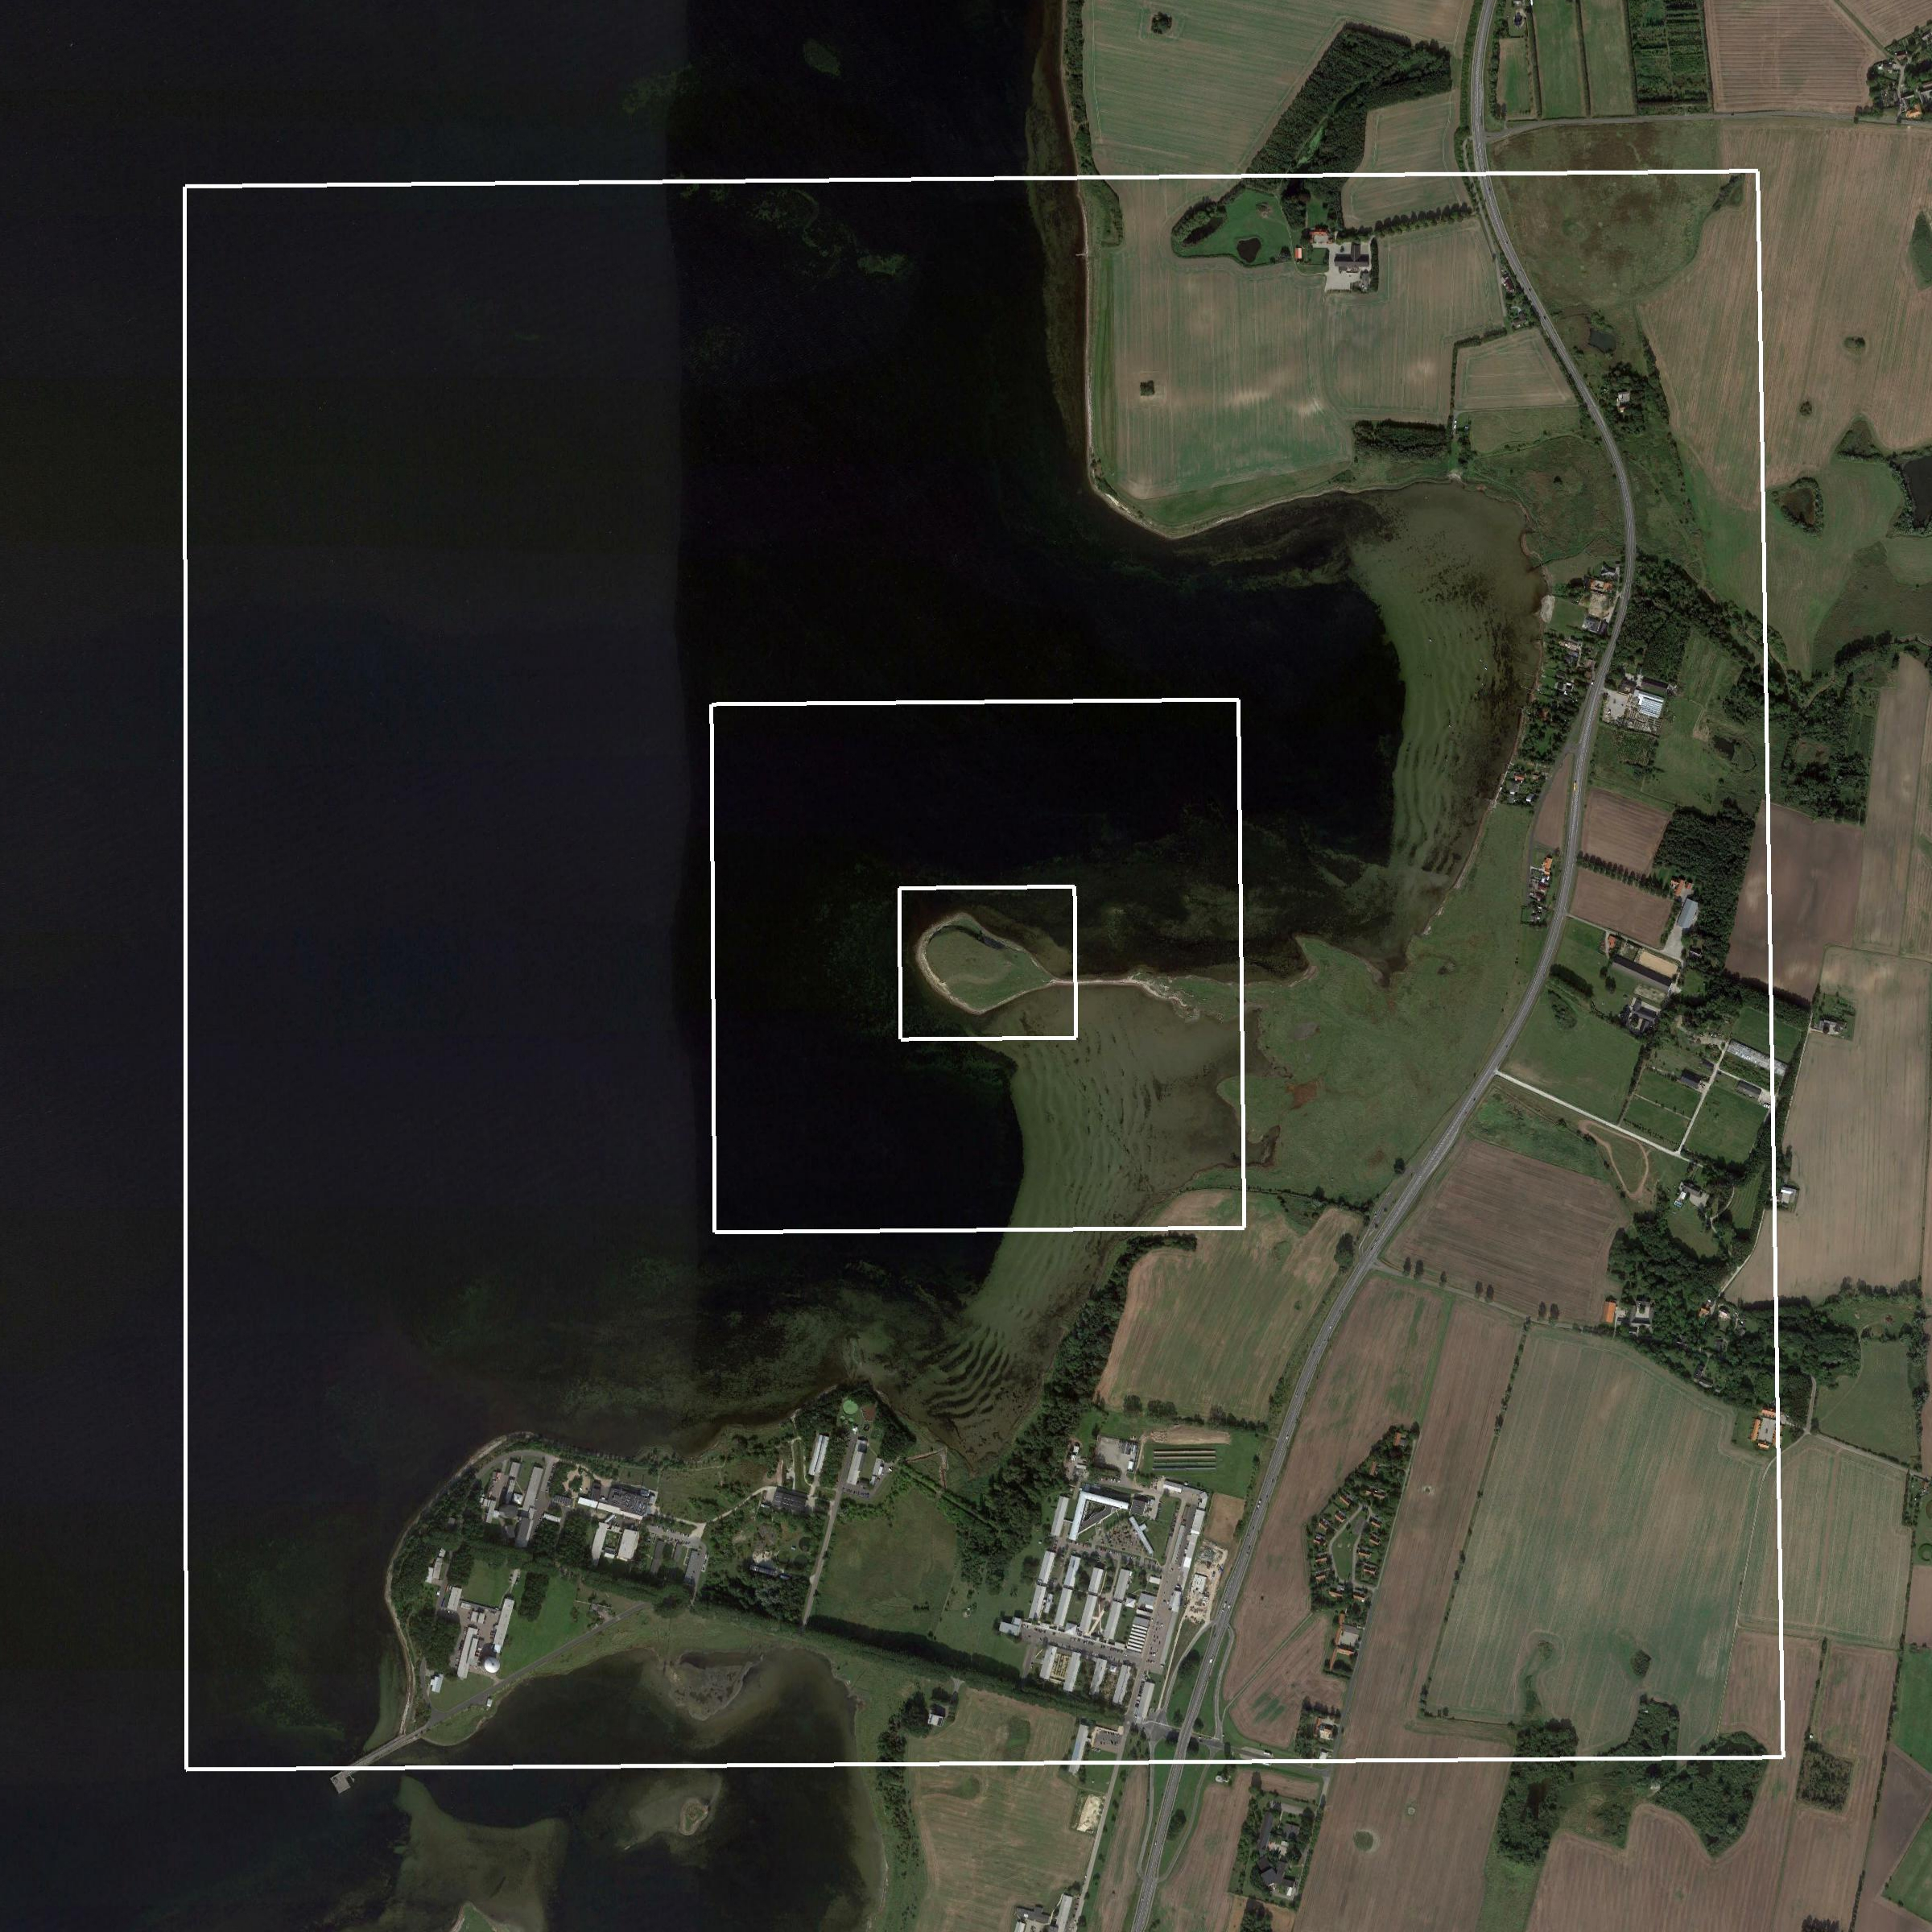
\includegraphics[width=0.48\linewidth,page=1,trim={5mm 3mm 3mm 3mm},clip,frame]{fig/05/bol_d6-7-8edit.jpg}%
		
		\caption{Distribución telescópica de las 8 mallas anidadas en el dominio numérico de la colinda Bolund.}
		\label{fig:05_dom_bol}
	\end{figure}
\end{frame}

\begin{frame}{Metodología}{Configuración: Caso II Bolund}
	\begin{figure}[H]
		\centering
		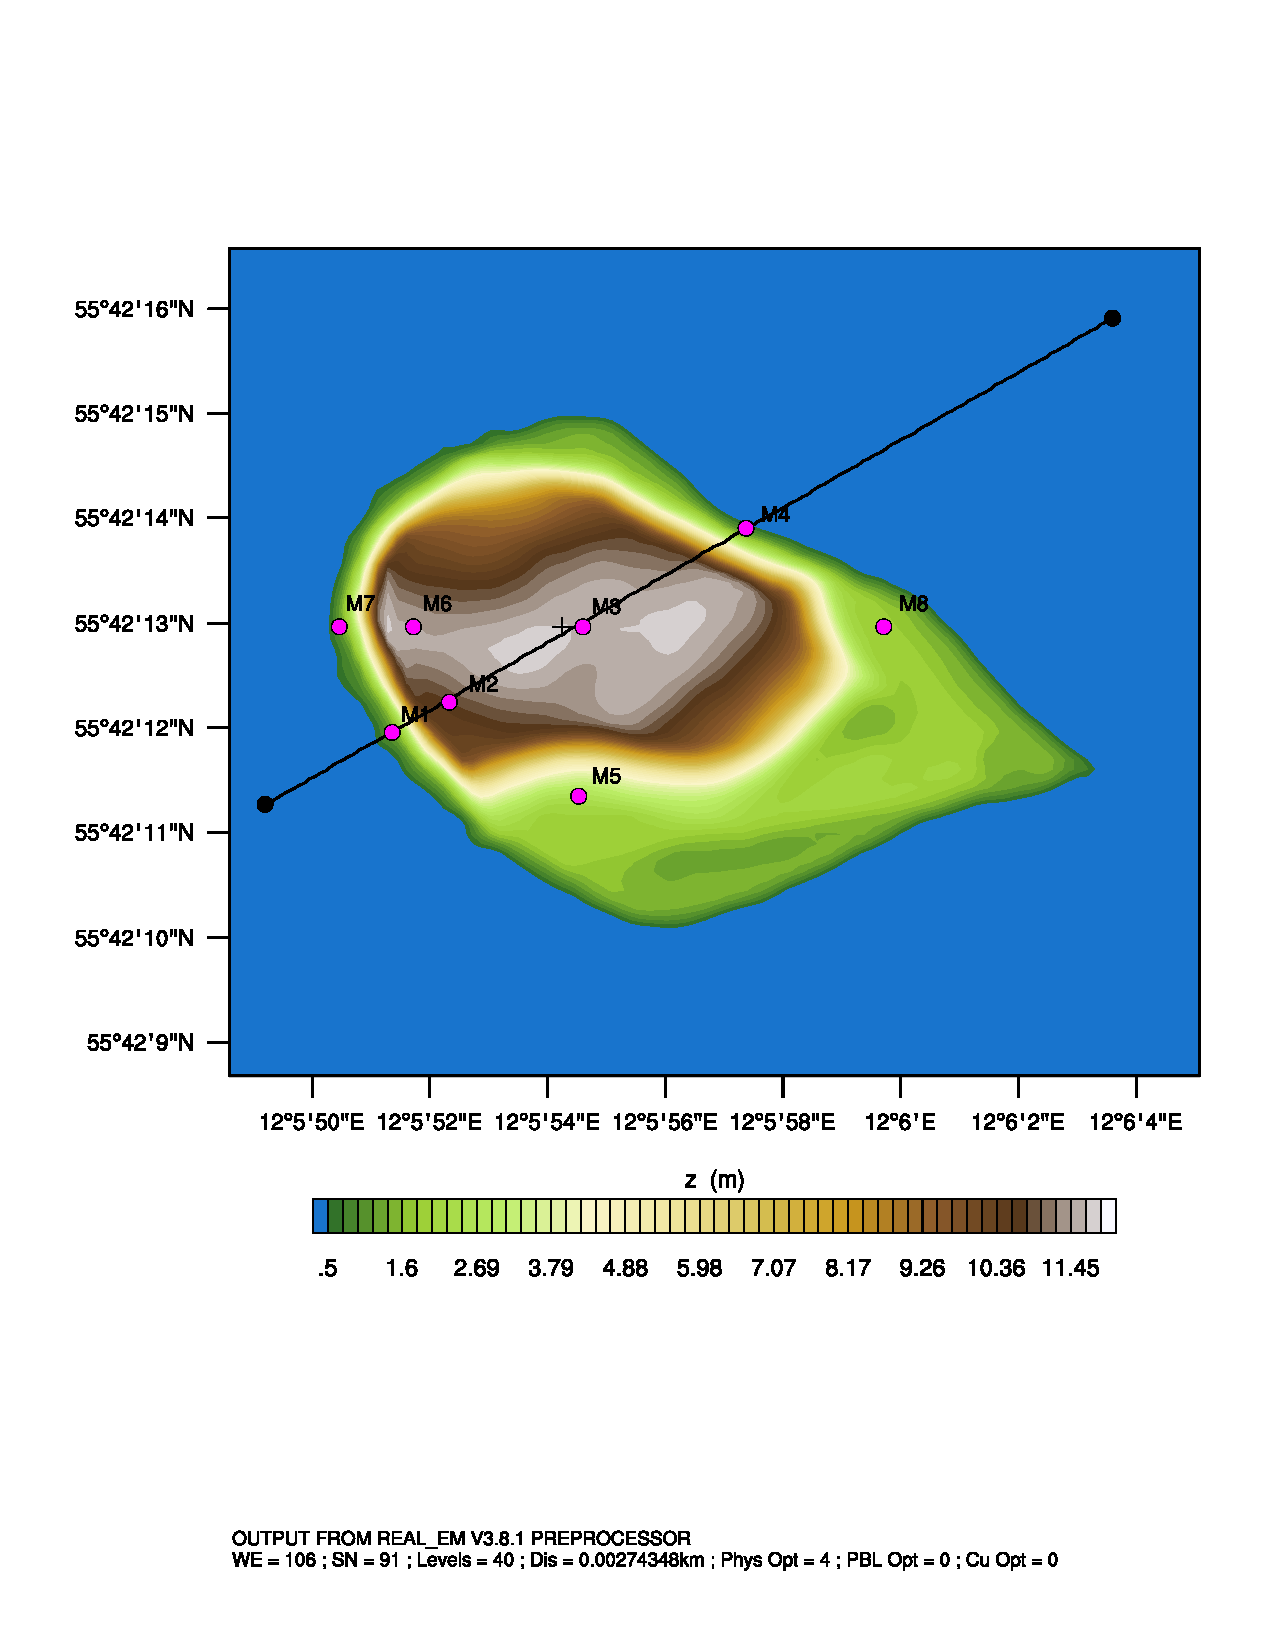
\includegraphics[width=0.75\linewidth,page=1,trim={0cm 6cm -1cm 4cm},clip]{fig/05/bol_control_point.pdf}%
		\vspace{-2mm}
		\caption{Ubicación espacial de los puntos de control en el dominio de Bolund. En cada punto de control se ubican anemómetros que miden a las alturas de 2m, 5m, y 9m sobre el suelo.}
		\label{fig:05_d08_bol}
	\end{figure}
\end{frame}

\begin{frame}{Metodología}{Configuración: Caso II Bolund}
	\begin{figure}[H]
		\centering
		\begin{minipage}{0.5\linewidth}
			\center\hspace{1.2cm}(a)
		\end{minipage}%
		\begin{minipage}{0.5\linewidth}
			\center(b)
		\end{minipage}%
		
		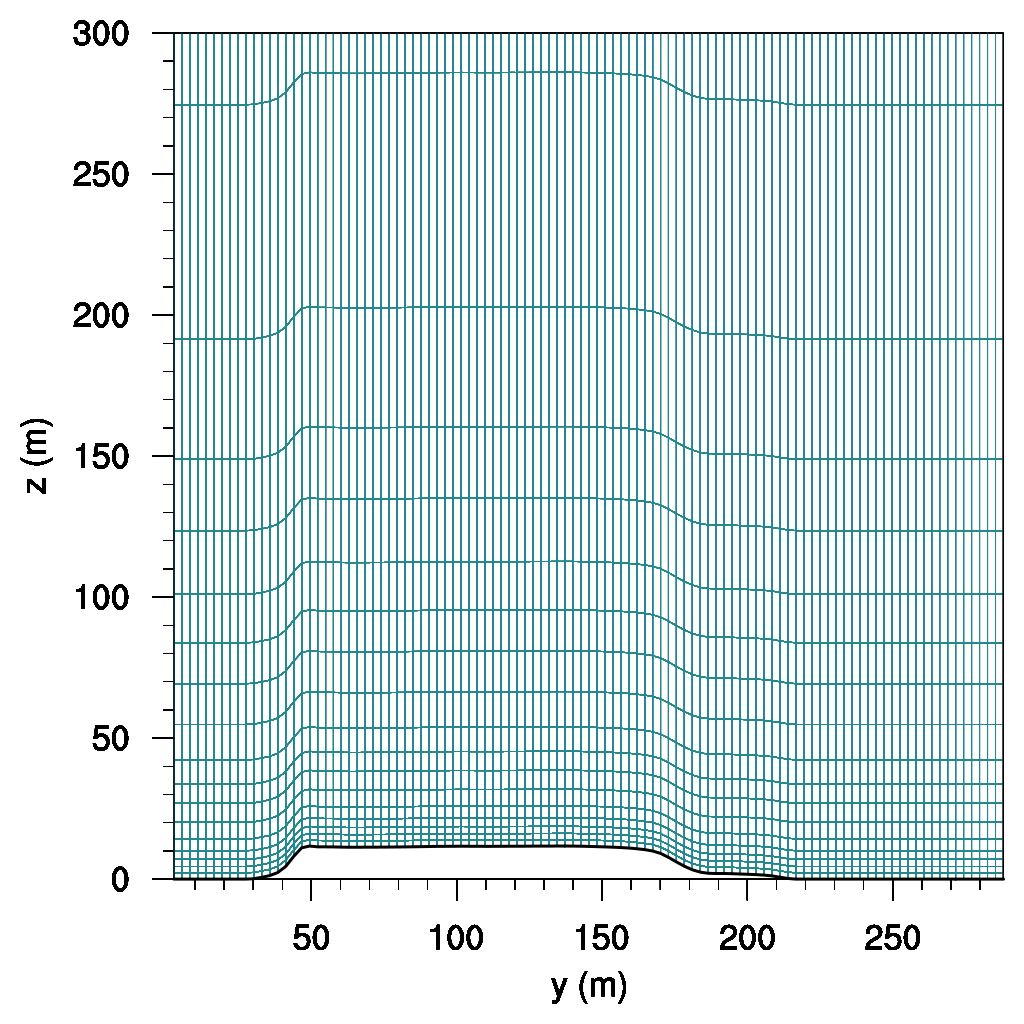
\includegraphics[width=0.45\linewidth,trim={0cm 0cm -0cm 0cm},clip]{fig/05/mesh_y50}%
		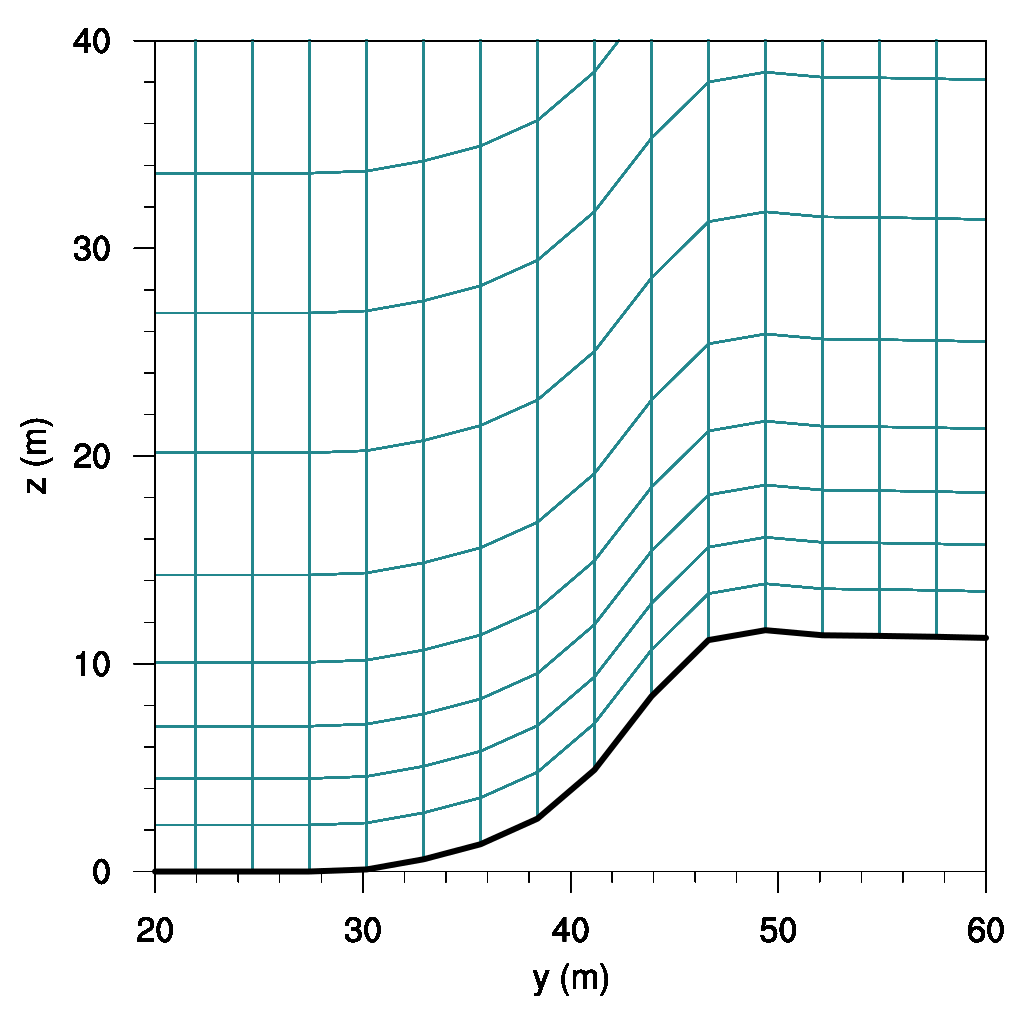
\includegraphics[width=0.45\linewidth,trim={0cm 0cm 0cm 0cm},clip]{fig/05/hd_mesh_50}%
		
		\caption{(a) Distribución de la malla vertical en la mitad del dominio en Bolund. (b) Detalle la pendiente abrupta (escala 1:1).}
		\label{fig:05_mesh_bol}
	\end{figure}
\end{frame}

\begin{frame}{Metodología}{Configuración: Caso II Bolund}
	\begin{table}[h!]
		\caption{Dominio numérico espacial y temporal para simulación del caso Bolund.}\label{tab:05_config_bol}
		\centering\footnotesize
		\begin{tabular}{lcc}
			\toprule
			Parámetro & Selección \\
			\midrule
			Fecha	 	 & 29-12-2007   \\
			Hora Inicio	 	 & 06:00 UTM\\
			Hora Término	 		 & 15:00 UTM\\
			Puntos Malla Vert.	 	 & 41   \\
			$P_{top}$ 	& 30000 [Pa]\\
			\# Dominios	& 8   \\
			Lat. Centro	& 55.703474   \\
			Lon. Centro	& 12.098854   \\
			Interválo Salida & 5 [min]\\
			Punto de Malla Total & 3,465,000\\
			\bottomrule
		\end{tabular}
	\end{table}
\end{frame}

\begin{frame}{Metodología}{Configuración: Caso II Bolund}
	\vspace{-4mm}
	\begin{table}[h!]
		\caption{Valores característicos de cada dominio en Bolund.}\label{tab:05_caract_bol}
		\vspace{-5mm}
		\centering\footnotesize\resizebox{\textwidth}{!}{
			\begin{tabular}{lcccccccc}
				\toprule
				Dominio 				& d01	&	d02	&	d03	&	d04	&	d05	&	d06 &	d07&	d08 \\
				\midrule
				$N_x$		& 106 & 106 & 106 &106&106&106&106&106  \\
				$N_y$	 		& 106 & 106 & 106 &106&106&106&106&91  \\
				$\Delta x, y$	[m]	 		& 10000 & 3333.3 & 1111.1 &222.22&74.074&24.691&8.23045&2.74348  \\
				$\Delta t$	[s]	 		& 12 & 4 & 1.3333 &0.4444&0.0889&0.0296&0.0099&0.0033  \\
				Orografía		 	& GMTED & GMTED & GMTED &ASTER&ASTER&ASTER&ASTER&Bolund  \\
				Uso de Suelo		& USGS & USGS & USGS &CLC12&CLC12&CLC12&CLC12&Bolund \\
				\bottomrule
			\end{tabular}}
	\end{table}
	\vspace{-4mm}
	\begin{table}[h!]
		\caption{Parametrizaciones físicas utilizadas en el modelo para Bolund.}\label{tab:05_param_bol}
		\vspace{-5mm}
		\centering\footnotesize\resizebox{\textwidth}{!}{
		\begin{tabular}{lcccccccc}
			\toprule
			Dominio 				& d01	&	d02	&	d03	&	d04	&	d05	&	d06 &	d07& d08\\
			\midrule
			Micro-físicas		 	& WSM5 & WSM5 & WSM5 &WSM5&WSM5&WSM5&WSM5& WSM5 \\
			Cúmulos			 		& Grell & -- & -- & -- & -- & -- & -- & -- \\ 
			Capa Superficial	 	& MYNN & MYNN & MYNN & MYNN & MYNN & MYNN & MYNN& MYNN\\
			PBL				 		& MYNN & MYNN & MYNN & -- & -- & -- & -- &--\\
			Modelo LES				 		& -- & -- & -- & 1.5TKE & 1.5TKE & 1.5TKE & 1.5TKE& 1.5TKE \\
			$c_k$				 		& -- & -- & -- & $0.2$ & $0.2$ & $0.2$ & $0.2$& $0.2$ \\
			Modelo de Suelo 		& Difus. & Difus. & Difus. & Difus. & Difus. & Difus. & Difus.& Difus. \\
			Rad. Onda Larga	& RRTM &RRTM&RRTM&RRTM&RRTM&RRTM&RRTM& RRTM\\
			Rad. Onda Corta	& Dudhia &Dudhia&Dudhia&Dudhia&Dudhia&Dudhia&Dudhia& Dudhia\\
			\bottomrule
		\end{tabular}}
	\end{table}
\end{frame}	

%DATA ASIMILATION METODOLOGIA
\begin{frame}{Metodología}{Configuración de la Asimilación de Datos}
	\begin{figure}[H]
		\centering
		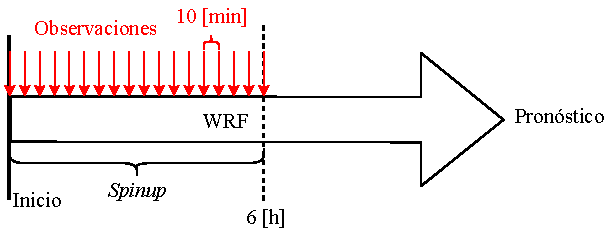
\includegraphics[width=0.95\linewidth,page=1,trim={0cm 0cm 0cm 0cm},clip]{fig/05/da}%
		\caption{Esquema del proceso de asimilación de datos.}
		\label{fig:05_da}
	\end{figure}
\end{frame}

\begin{frame}{Metodología}{Configuración de la Asimilación de Datos}
	\begin{table}[h!]
		\caption{Características del proceso de DA en Høvsøre.}\label{tab:05_config_da_hov}
		\centering\footnotesize
		\begin{tabular}{lcc}
			\toprule
			Parámetro & Selección \\
			\midrule
			Hora Inicio	DA 	 & 06:00:00   \\
			Hora Término DA	 		 & 12:00:00  \\
			Intervalo de DA	&	10 [min] \\
			Puntos a Anidar	 	 & 1   \\
			Alturas 	& 10m, 40m, 60m, 80m, 100m \\
			Variables	& $u,v$   \\
			Lat. Mástil	& 56.440582   \\
			Lon. Mástil	& 8.150896   \\
			
			\bottomrule
		\end{tabular}
	\end{table}
	
	\begin{table}[H]
		\caption{Detalle de la asimilación en cada mástil en Bolund.}\label{tab:05_mast_da_bol}
		\vspace{-4mm}
		\centering\footnotesize\resizebox{\textwidth}{!}{
			\begin{tabular}{lcccccccc}
				\toprule
				& M1	&	M2	&	M3	&	M4	&	M5	&	M6 &	M7	& M8\\
				\midrule
				Latitud		 	& 55.70332 & 55.70340 & 55.70360 & 55.70386 & 55.70315 & 55.70360 & 55.70360 & 55.70360 \\
				Longitud	    & 12.09760 & 12.09787 & 12.09850 & 12.09927 & 12.09848 & 12.09770 & 12.09735 & 12.09992 \\
				Alturas			& 2, 5, 9m & 2, 5m & 2, 5m & 2, 5, 9m & 2, 5m & 2, 5m & 2, 5m & 2, 5m \\
				
				\bottomrule
			\end{tabular}}
		\end{table}
\end{frame}

\begin{frame}{Metodología}{Configuración de la Asimilación de Datos}
	\begin{figure}[H]
		\centering
		\begin{minipage}{0.5\linewidth}
			\center\hspace{0.3cm}(a)
		\end{minipage}%
		\begin{minipage}{0.5\linewidth}
			\center\hspace{0.3cm}(b)
		\end{minipage}%
		
		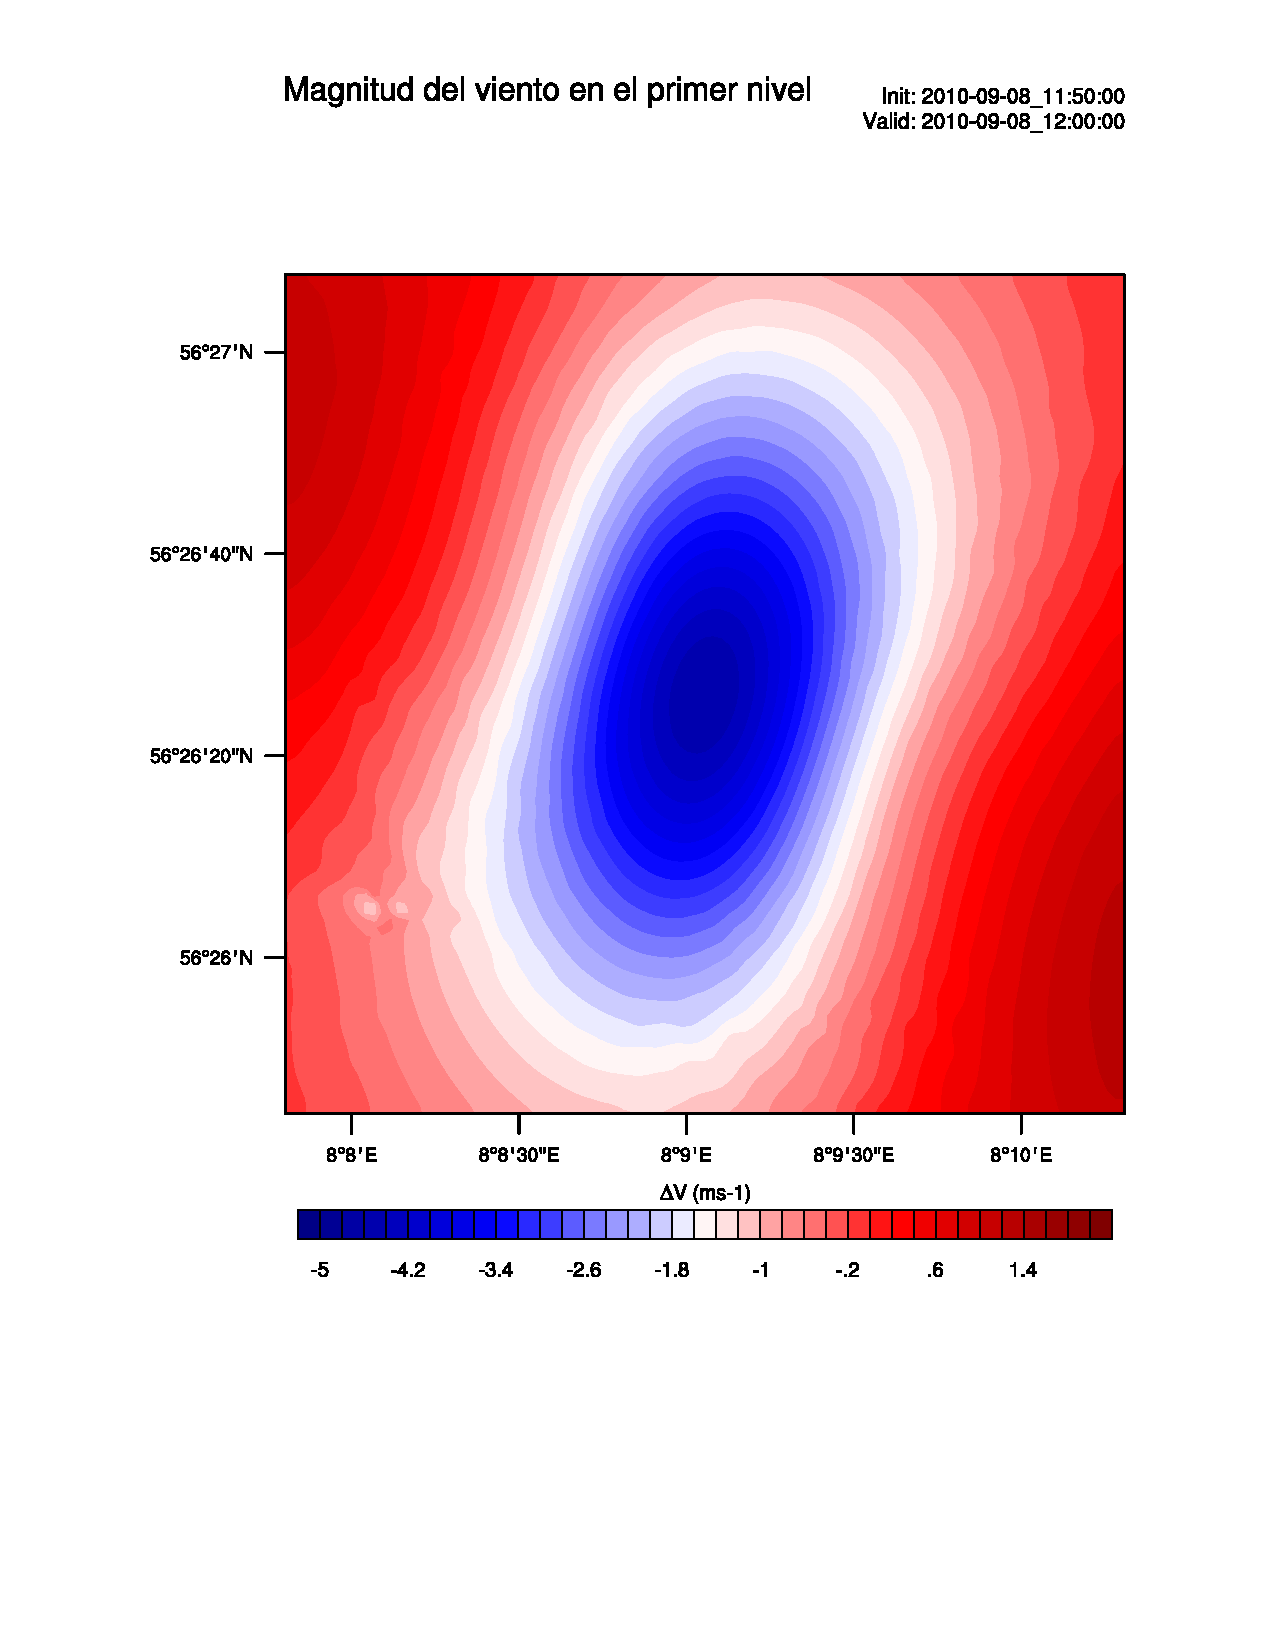
\includegraphics[width=0.5\linewidth,page=1,trim={2.5cm 6.2cm 1cm 4.5cm},clip]{fig/05/eta1_da_hov}%
		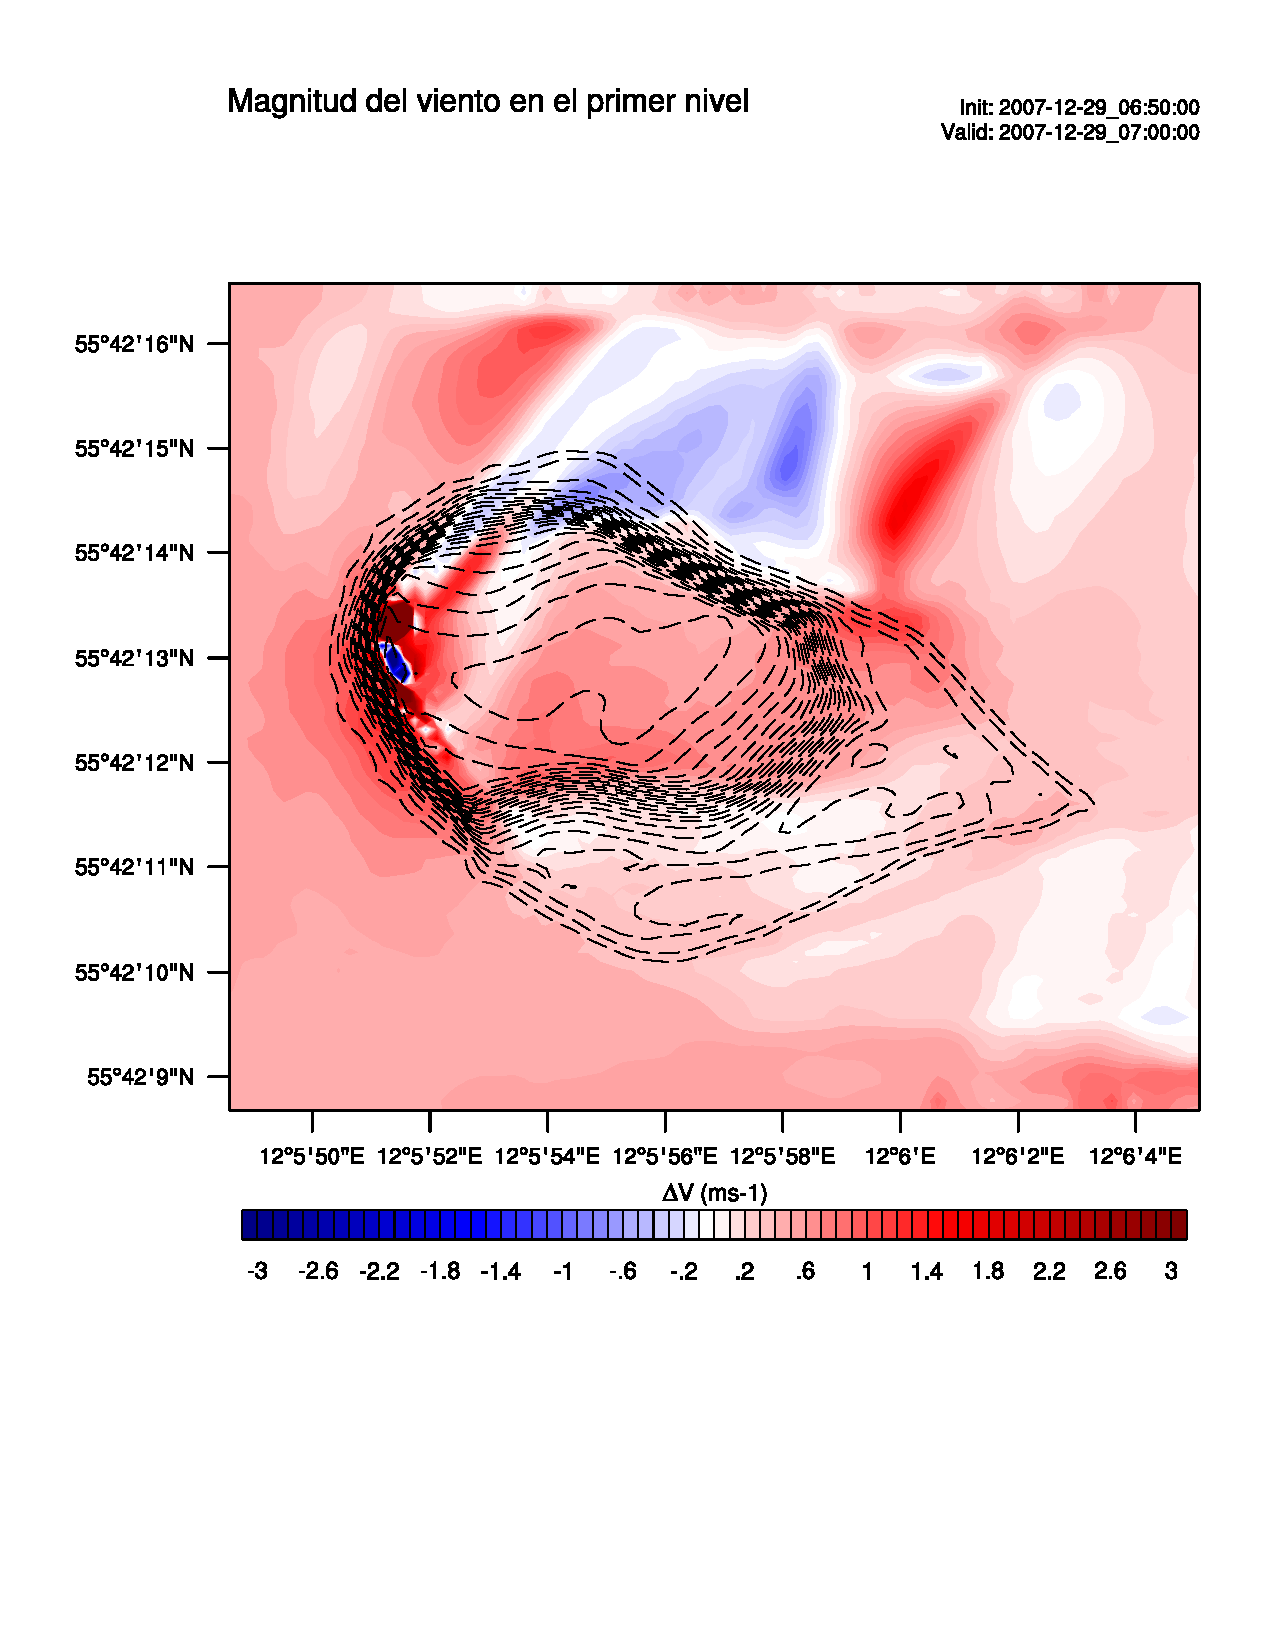
\includegraphics[width=0.5\linewidth,page=1,trim={1.0cm 5.2cm 1cm 4.5cm},clip]{fig/05/eta1_da_bol}%
		\caption{Diferencia de la magnitud del campo de velocidad en el primer nivel del modelo entre resultados sin y con asimilación de datos. (a) Caso I puntual. (b) Caso II con varios puntos.}
		\label{fig:05_da_expl}
	\end{figure}
\end{frame}

\begin{frame}{Metodología}{Estimación del Error}
	MAE:
	\be E_1=\frac{1}{n}\sum_{i=1}^n |y_i-x_i| \ee
	RMSE:
	\be E_2=\sqrt{\frac{1}{n}\sum_{i=1}^n (y_i-x_i)^2} \ee
	Coeficiente de Pearson:
	\be r =\frac{\sum\limits_{i=1}^n [(x_i-\overline{x})(y_i-\overline{y})]} {\left[\sum\limits_{i=1}^n (x_i-\overline{x})^2\right]^{1/2} \left[\sum\limits_{i=1}^n (y_i-\overline{y})^2\right]^{1/2}} \ee
\end{frame}








%RESULTADOS
%EXP 1
\section{7. Resultados}
\begin{frame}{Resultados}{Caso I: Høvsøre - Validación}
	\begin{figure}[H]
		\begin{minipage}{0.5\linewidth}
			\centering
			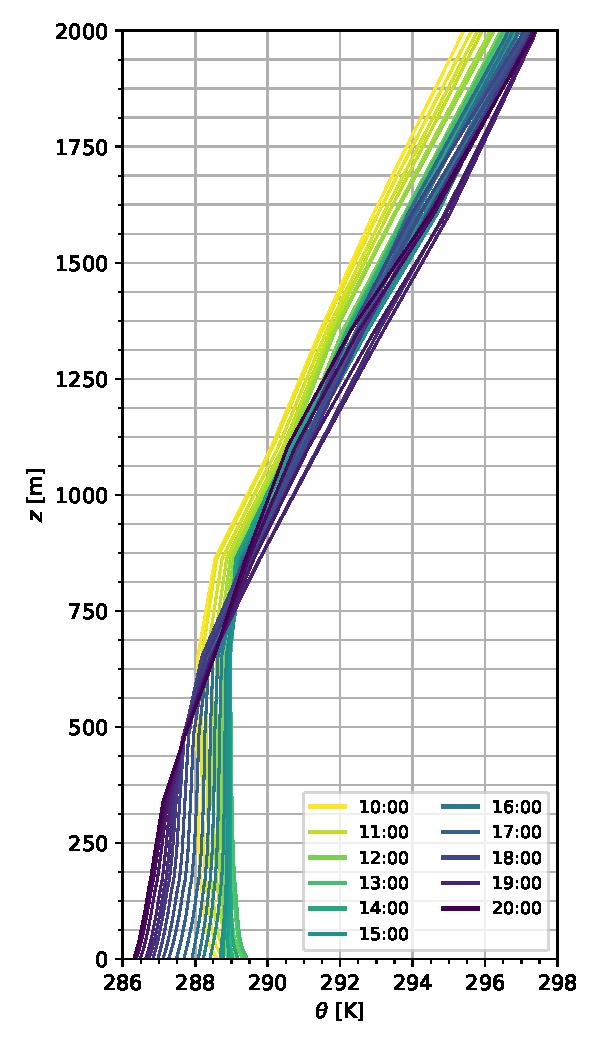
\includegraphics[width=0.75\linewidth,trim={0cm 5mm 0cm 0mm},clip]{fig/06/hov/pbl}%
		\end{minipage}%
		\begin{minipage}{0.5\linewidth}
			\centering
			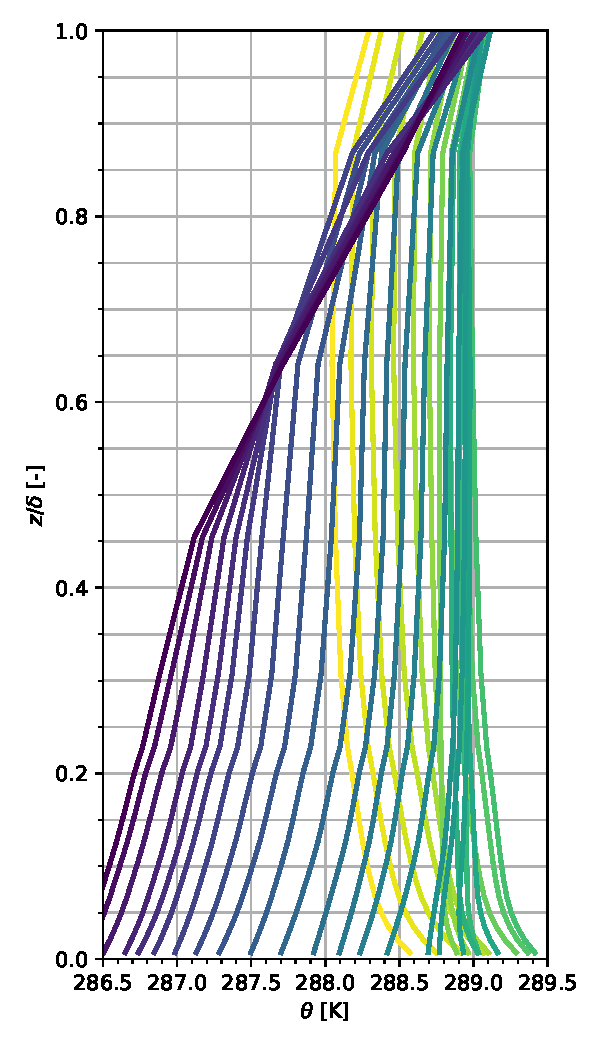
\includegraphics[width=0.75\linewidth,trim={0cm 5mm 0cm 0cm},clip]{fig/06/hov/temp_profile}%
		\end{minipage}%
		
		\caption{Perfil de temperatura potencial virtual en Høvsøre ($\delta \approx 750$ [m]).}
		\label{fig:06_hov_pbl}
	\end{figure}
\end{frame}

\begin{frame}{Resultados}{Caso I: Høvsøre - Validación}
	\begin{figure}[H]
		\centering
		\includegraphics[width=0.6\linewidth,page=55,trim={2.5cm 6.2cm 1cm 4.5cm},clip]{fig/06/hov/eta1_V}%
		\caption{Magnitud de la velocidad en el primer nivel de la coordenada vertical ($z_1=5.25$ [m]) para las 15:00.}
		\label{fig:06_hov_eta1}
	\end{figure}
\end{frame}

\begin{frame}{Resultados}{Caso I: Høvsøre - Validación}
	\begin{figure}[H]
		\centering
		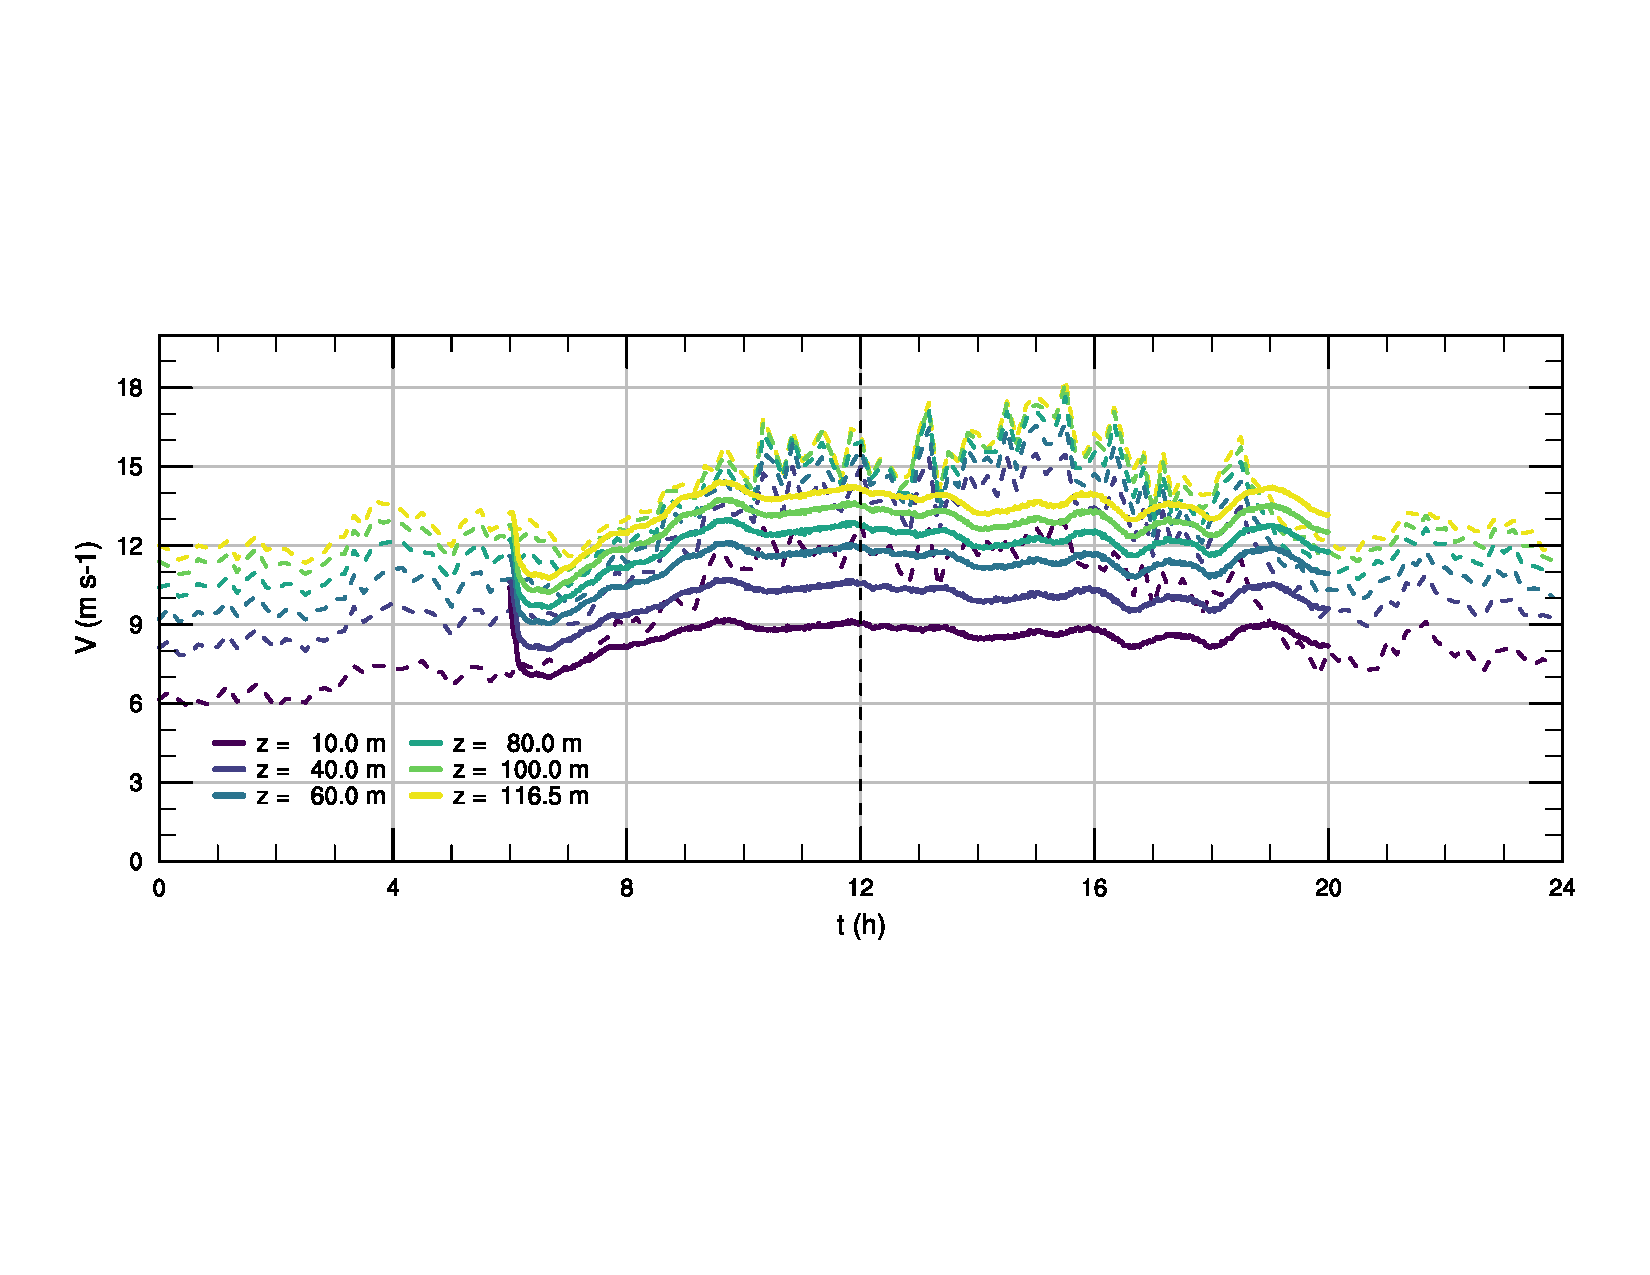
\includegraphics[width=0.85\linewidth,trim={9mm 63mm 10mm 55mm},clip]{fig/06/hov/ts_v}%
		
		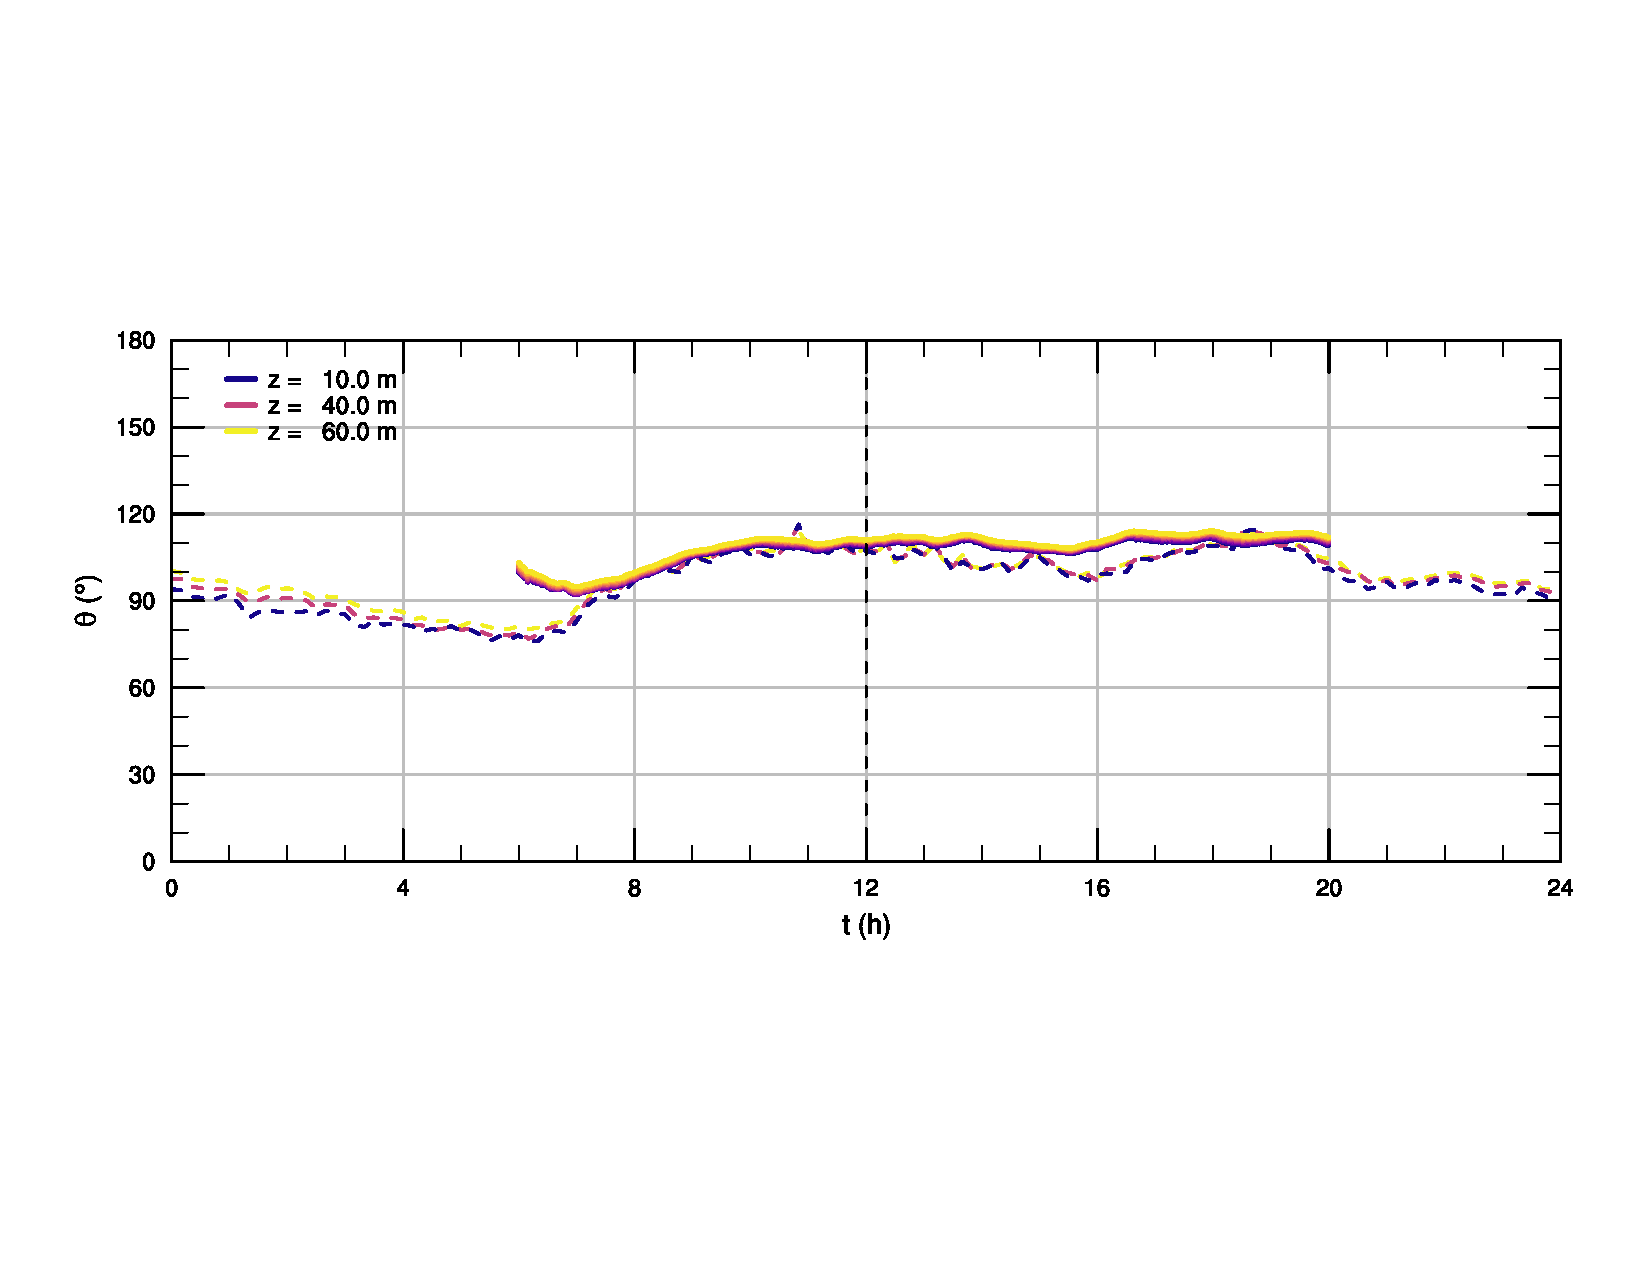
\includegraphics[width=0.85\linewidth,trim={12mm 55mm 10mm 55mm},clip]{fig/06/hov/ts_o}%
		\vspace{-4mm}
		\caption{Serie de tiempo para la solución caso Høvsøre.}
		\label{fig:06_hov_ts}
	\end{figure}
\end{frame}

\begin{frame}{Resultados}{Caso I: Høvsøre - Validación}
	\vspace{-3mm}
	\begin{figure}[h!]
		\begin{center}
			\includegraphics[height=0.6\linewidth,page=37,trim={35mm 10mm 41mm 25mm},clip]{fig/06/hov/9u}%
			\includegraphics[height=0.6\linewidth,page=37,trim={48mm 10mm 41mm 25mm},clip]{fig/06/hov/9v}%
			\includegraphics[height=0.6\linewidth,page=37,trim={48mm 10mm 20mm 25mm},clip]{fig/06/hov/9V}%
		\end{center}
		\vspace{-3mm}
		\caption{Validación con Peña et al. (2013). Valores promedios entre las 12:00 y 15:00.}
		\label{fig:06_hov_pea}
	\end{figure}
\end{frame}

\begin{frame}{Resultados}{Caso I: Høvsøre - Validación}
	\begin{figure}[H]
		\begin{center}
			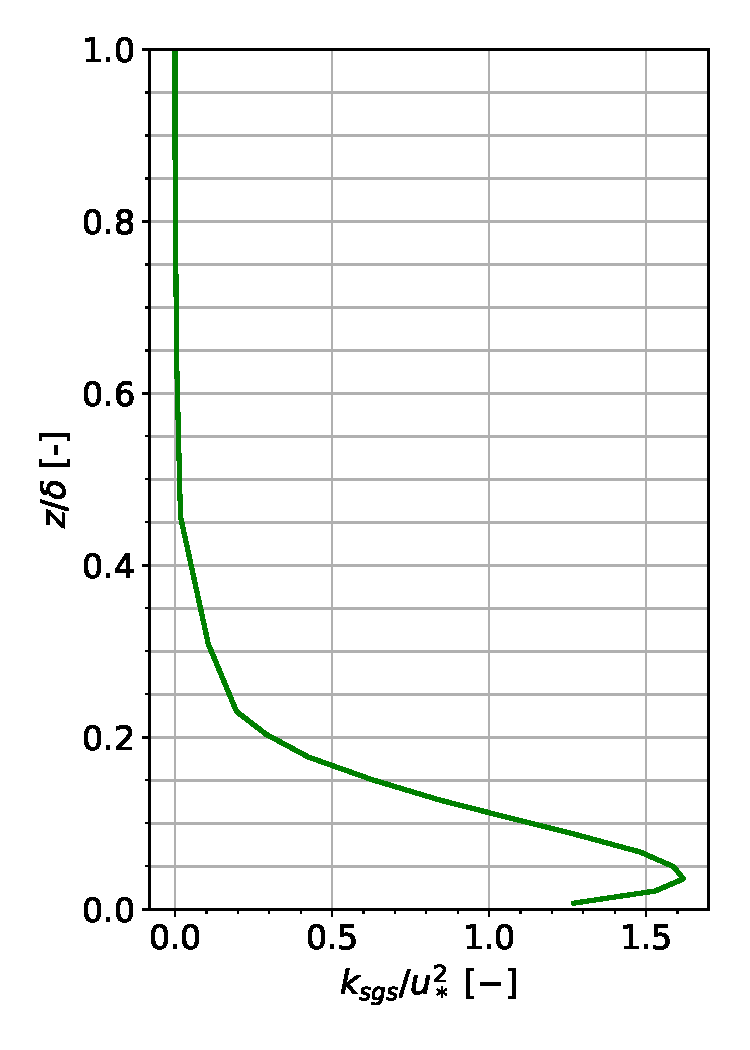
\includegraphics[height=0.5\linewidth,page=1,trim={6mm 5mm 3mm 0mm},clip]{fig/06/hov/mean_data}%
			\includegraphics[height=0.5\linewidth,page=2,trim={12mm 5mm 3mm 0mm},clip]{fig/06/hov/mean_data}%
			\includegraphics[height=0.5\linewidth,page=3,trim={12mm 5mm 0mm 0mm},clip]{fig/06/hov/mean_data}%
		\end{center}
		\caption{Variables de segundo orden adimensionalizadas. Promedios entre las 12:00 y 15:00 ($u_* = 0.552$ [m/s]). }
		\label{fig:06_hov_mean_secondorder}
	\end{figure}
\end{frame}

\begin{frame}{Resultados}{Caso I: Høvsøre - Validación}
	\begin{figure}[H]
		\centering
		\hspace*{-5mm}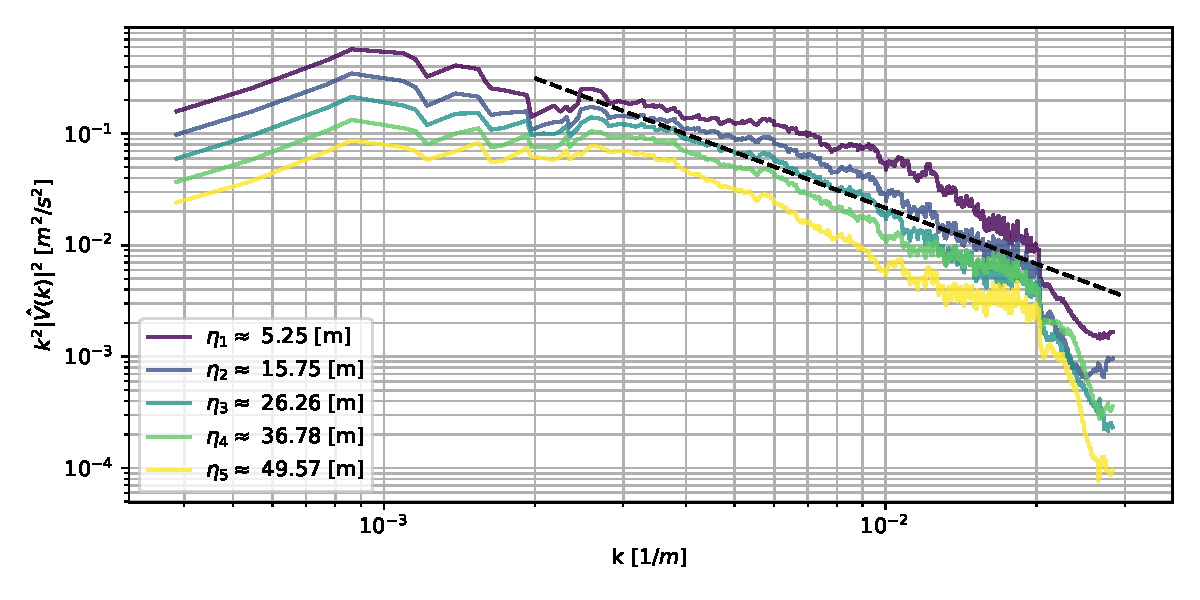
\includegraphics[width=1.1\linewidth,page=1,trim={3mm 5mm -7mm 3mm},clip]{fig/06/hov/spectra}%
		%\vspace{-3mm}
		\caption{Espectros de energía cinética para la magnitud horizontal del viento a distintos niveles verticales en el dominio d07 caso Høvsøre.}
		\label{fig:06_hov_spectrum}
	\end{figure}
\end{frame}

\begin{frame}{Resultados}{Caso I: Høvsøre - Validación}
	\[ \boxed{\text{MAE} = 2.41091 \text{ [m/s]} \quad;\quad \text{RMSE} = 2.80142 \text{ [m/s]}} \]
	\begin{figure}[H]
		\centering
		\vspace{-3mm}
		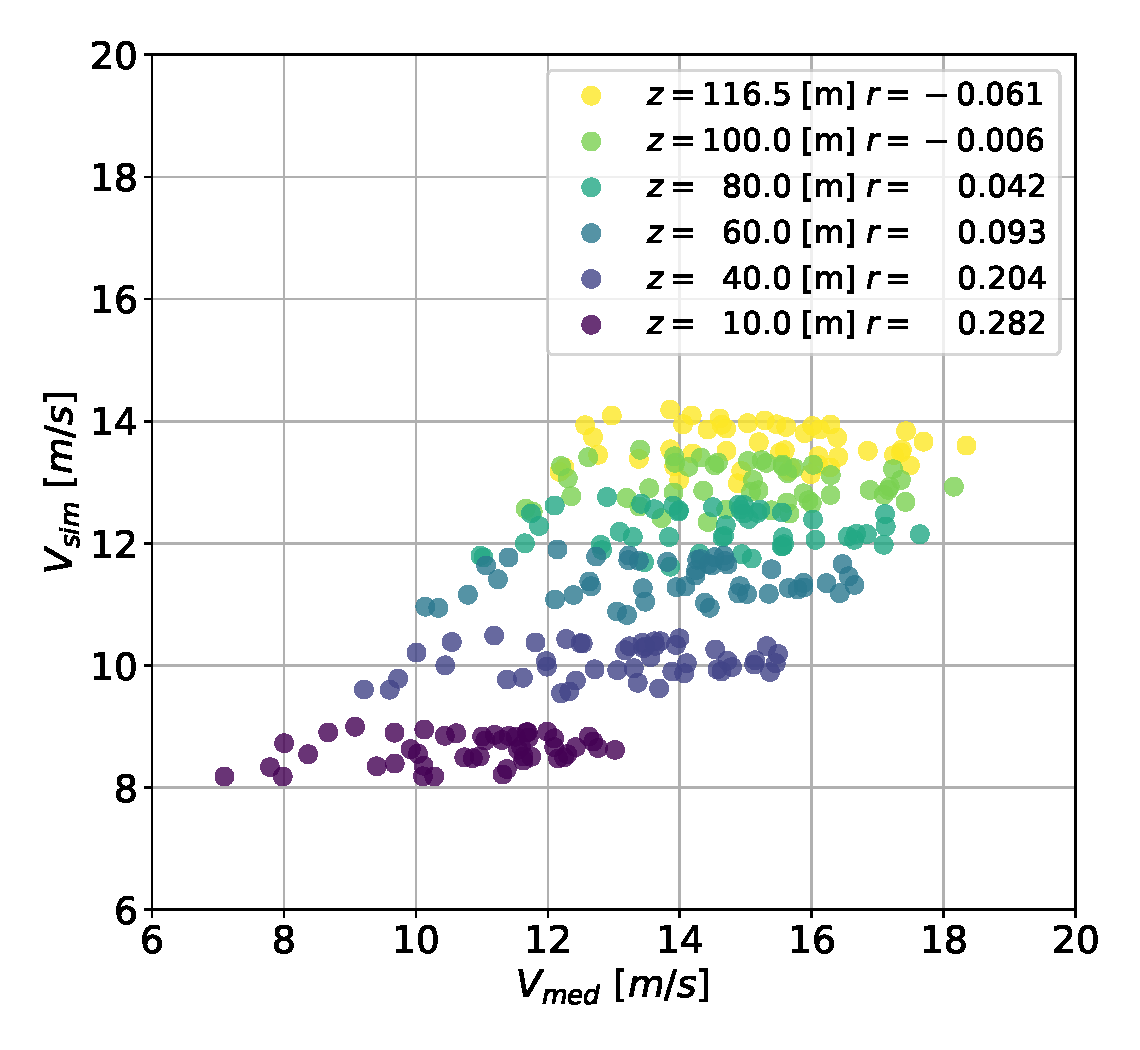
\includegraphics[width=0.6\linewidth,page=1,trim={0cm 5mm -1cm 0cm},clip]{fig/06/hov/corr}%
		\vspace{-3mm}
		\caption{Gráfico de dispersión para las velocidades a distintas alturas en el mástil meteorológico de Høvsøre.}
		\label{fig:06_corr_hov}
	\end{figure}
\end{frame}
%HOVSORE DATA ASIMILATION










\begin{frame}{Resultados}{Caso I: Høvsøre - Asimilación de Datos}
	\begin{figure}[H]
		\centering
		\includegraphics[width=0.85\linewidth,trim={9mm 63mm 10mm 55mm},clip]{fig/06/hov_da/ts_v}%
		
		\includegraphics[width=0.85\linewidth,trim={12mm 55mm 10mm 55mm},clip]{fig/06/hov_da/ts_o}%
		\vspace{-4mm}
		\caption{Serie de tiempo para la solución caso Høvsøre.}
		\label{fig:06_hov_da_ts}
	\end{figure}
\end{frame}

\begin{frame}{Resultados}{Caso I: Høvsøre - Asimilación de Datos}
	\vspace{-3mm}
	\begin{figure}[h!]
		\begin{center}
			\includegraphics[height=0.6\linewidth,page=37,trim={35mm 10mm 41mm 25mm},clip]{fig/06/hov_da/9u}%
			\includegraphics[height=0.6\linewidth,page=37,trim={48mm 10mm 41mm 25mm},clip]{fig/06/hov_da/9v}%
			\includegraphics[height=0.6\linewidth,page=37,trim={48mm 10mm 20mm 25mm},clip]{fig/06/hov_da/9V}%
		\end{center}
		\vspace{-3mm}
		\caption{Validación con Peña et al. (2013). Valores promedios entre las 12:00 y 15:00.}
		\label{fig:06_hov_da_pea}
	\end{figure}
\end{frame}

\begin{frame}{Resultados}{Caso I: Høvsøre - Asimilación de Datos}
	\begin{figure}[H]
		\begin{center}
			\includegraphics[height=0.5\linewidth,page=1,trim={6mm 5mm 3mm 0mm},clip]{fig/06/hov_da/mean_data}%
			\includegraphics[height=0.5\linewidth,page=2,trim={12mm 5mm 3mm 0mm},clip]{fig/06/hov_da/mean_data}%
			\includegraphics[height=0.5\linewidth,page=3,trim={12mm 5mm 0mm 0mm},clip]{fig/06/hov_da/mean_data}%
		\end{center}
		\caption{Variables de segundo orden adimensionalizadas. Promedios entre las 12:00 y 15:00 ($u_* = 0.527$ [m/s]). }
		\label{fig:06_hov_da_mean_secondorder}
	\end{figure}
\end{frame}

\begin{frame}{Resultados}{Caso I: Høvsøre - Asimilación de Datos}
	\begin{figure}[H]
		\centering
		\hspace*{-5mm}\includegraphics[width=1.1\linewidth,page=1,trim={3mm 5mm -7mm 3mm},clip]{fig/06/hov_da/spectra}%
		%\vspace{-3mm}
		\caption{Espectros de energía cinética para la magnitud horizontal del viento a distintos niveles verticales en el dominio d07 caso Høvsøre.}
		\label{fig:06_hov_da_spectrum}
	\end{figure}
\end{frame}

\begin{frame}{Resultados}{Caso I: Høvsøre - Asimilación de Datos}
	\begin{figure}[H]
		\centering
		%\vspace{-3mm}
		\includegraphics[width=0.7\linewidth,page=1,trim={0cm 5mm -1cm 0cm},clip]{fig/06/hov_da/corr}%
		\vspace{-3mm}
		\caption{Gráfico de dispersión para las velocidades a distintas alturas en el mástil meteorológico de Høvsøre.}
		\label{fig:06_corr_hov_da}
	\end{figure}
\end{frame}

\begin{frame}{Resultados}{Caso I: Høvsøre - Síntesis}
	%\begin{minipage}{0.5\linewidth}
		Observaciones relevantes:
		\begin{itemize}
			\item Los resultados con Peña validan la metodología.
			\item El LES funciona de buena manera.
			\item El modelo es muy difusivo en los primeros niveles.
			\item Las variables de 2do orden se comportan según lo esperado, salvo $\Phi_M$.
			\item La asimilación de datos presenta mejoras en los estadísticos.
		\end{itemize}
	%\end{minipage}%
	%\begin{minipage}{0.5\linewidth}
		\begin{table}[H]
			\caption{Comparación de métricas para el caso I Høvsøre.}
			\label{tab:06_hov_mae_rmse}
			\centering%\footnotesize
			%\resizebox{\textwidth}{!}{
			\begin{tabular}{lcc}
				\toprule
				& Sin DA & Con DA \\
				\midrule
				MAE & 2.41 m/s & 2.17 m/s \\
				RMSE & 2.80 m/s& 2.56 m/s\\
				$\Delta{RMSE}$& --  & $8.70\%$  \\
				$\Delta{MAE}$ & -- & $10.47\%$  \\
				\bottomrule
			\end{tabular}
		\end{table}
	%\end{minipage}%
\end{frame}





%BOLUND SIN DA
\begin{frame}{Resultados}{Caso II: Bolund}
	\begin{figure}[H]
		\begin{minipage}{0.5\linewidth}
			\centering
			\includegraphics[width=0.75\linewidth,trim={0cm 5mm 0cm 0mm},clip]{fig/06/bol/mean_pbl}%
		\end{minipage}%
		\begin{minipage}{0.5\linewidth}
			\centering
			\includegraphics[width=0.75\linewidth,trim={0cm 5mm 0cm 0cm},clip]{fig/06/bol/mean_profile}%
		\end{minipage}%
		
		\caption{Perfil de temperatura potencial virtual en Bolund ($\delta\approx 300$ [m]).}
		\label{fig:06_bol_pbl}
	\end{figure}
\end{frame}

\begin{frame}{Resultados}{Caso II: Bolund}
	\begin{figure}[H]
		\begin{minipage}{0.5\linewidth}
			\centering
			\includegraphics[height=0.55\linewidth,page=73,trim={12mm 31mm 50mm 20mm},clip]{fig/06/bol/eta1}%
		\end{minipage}%
		\begin{minipage}{0.5\linewidth}
			\centering
			\includegraphics[height=0.55\linewidth,page=85,trim={37mm 31mm 20mm 20mm},clip]{fig/06/bol/eta1}%
		\end{minipage}%
		\vspace{1mm}
		
		\begin{minipage}{0.5\linewidth}
			\centering
			\includegraphics[height=0.57\linewidth,page=97,trim={12mm 23mm 50mm 20mm},clip]{fig/06/bol/eta1}%
		\end{minipage}%
		\begin{minipage}{0.5\linewidth}
			\centering
			\includegraphics[height=0.57\linewidth,page=109,trim={37mm 23mm 20mm 20mm},clip]{fig/06/bol/eta1}%
		\end{minipage}%
		\caption{Líneas de flujo para la solución en Bolund en el primer nivel ($z_1 = 1.12$ [m]) para (a) 12:00, (b) 13:00, (c) 14:00 y (d) 15:00.}
		\label{fig:06_bol_st}
	\end{figure}
\end{frame}

\begin{frame}{Resultados}{Caso II: Bolund}
	\begin{figure}[H]
		\centering
		\includegraphics[width=0.80\linewidth,trim={0mm 202.0mm 111mm 106mm},clip]{fig/06/bol/1200rot}\\%
		\includegraphics[width=0.80\linewidth,trim={0mm 202.0mm 111mm 106mm},clip]{fig/06/bol/1300rot}\\%
		\includegraphics[width=0.80\linewidth,trim={0mm 202.0mm 111mm 106mm},clip]{fig/06/bol/1400rot}\\%
		\includegraphics[width=0.80\linewidth,trim={0mm 180.0mm 111mm 106mm},clip]{fig/06/bol/1500rot}%
		\vspace{-2mm}
		\caption{Contornos de rapidez del viento para la sección de corte vertical a 240$^\circ$ en Bolund. 12:00 a 15:00. Escala 1:1.}
		\label{fig:06_bol_cross}
	\end{figure}
\end{frame}

\begin{frame}{Resultados}{Caso II: Bolund (Aceleración M1-M4)}
	\begin{figure}[H]
		\centering
		\includegraphics[width=0.65\linewidth,trim={12mm 84mm 10mm 74mm},page=1,clip]{fig/06/bol/speedup}\\%
		\includegraphics[width=0.65\linewidth,trim={12mm 84mm 10mm 74mm},page=13,clip]{fig/06/bol/speedup}\\%
		\includegraphics[width=0.65\linewidth,trim={12mm 84mm 10mm 74mm},page=25,clip]{fig/06/bol/speedup}\\%
		\includegraphics[width=0.65\linewidth,trim={12mm 84mm 10mm 74mm},page=37,clip]{fig/06/bol/speedup}\\%
		\includegraphics[width=0.65\linewidth,trim={-11mm 193mm 115mm 112mm},clip]{fig/06/bol/cross_height}\\%
		%\caption{Speedup en los primeros 3 niveles del modelo ($1.1$ [m] azul; $3.4$ [m] verde; $5.6$ [m] amarillo) para la sección de corte a 240$^\circ$ en Bolund. Se muestran los resultados para las 12:00 (arriba), 13:00, 14:00 y 15:00 horas (abajo).}
		\label{fig:06_bol_speedup}
	\end{figure}
\end{frame}

\begin{frame}{Resultados}{Caso II: Bolund (Delta TKE)}
	\begin{figure}[H]
		\centering
		\includegraphics[width=0.65\linewidth,trim={12mm 84mm 10mm 74mm},page=1,clip]{fig/06/bol/delta_tke}\\%
		\includegraphics[width=0.65\linewidth,trim={12mm 84mm 10mm 74mm},page=13,clip]{fig/06/bol/delta_tke}\\%
		\includegraphics[width=0.65\linewidth,trim={12mm 84mm 10mm 74mm},page=25,clip]{fig/06/bol/delta_tke}\\%
		\includegraphics[width=0.65\linewidth,trim={12mm 84mm 10mm 74mm},page=37,clip]{fig/06/bol/delta_tke}\\%
		\includegraphics[width=0.65\linewidth,trim={-13.3mm 193mm 115mm 112mm},clip]{fig/06/bol/cross_height}\\%
		%\caption{Incremento adimensional de energía cinética turbulenta (sgs) en los primeros 3 niveles del modelo ($1.1$ [m] azul; $3.4$ [m] verde; $5.6$ [m] amarillo) para la sección de corte a 240$^\circ$ en Bolund. Se muestran los resultados para las 12:00 (arriba), 13:00, 14:00 y 15:00 horas (abajo).}
		\label{fig:06_bol_tke}
	\end{figure}
\end{frame}

\begin{frame}{Resultados}{Caso II: Bolund}
	\begin{figure}[H]
		\centering
		\includegraphics[height=0.6\linewidth,page=1,trim={28mm 10mm 25mm 23mm},clip]{fig/06/bol/V_masts}%
		\includegraphics[height=0.6\linewidth,page=1,trim={30mm 10mm 17mm 20mm},clip]{fig/06/bol/k_masts}%
		\vspace{-2mm}\caption{Perfil vertical promedio de 12:00 a 15:00 de (a) \emph{speedup} y (b) variación adimensional de energía cinética turbulenta para las estaciones M1 (azul), M2 (naranja), M3 (verde) y M4 (rojo).}
		\label{fig:06_bol_mast_tke_speedup}
	\end{figure}
\end{frame}

\begin{frame}{Resultados}{Caso II: Bolund}
	\begin{figure}[H]
		\begin{minipage}{0.65\linewidth}
			\includegraphics[width=1.2\linewidth,page=1,trim={9mm 57mm 5mm 60mm},clip]{fig/06/bol/ts_interpol_compare.pdf}\\%
			\includegraphics[width=1.2\linewidth,page=1,trim={12mm 52mm 5mm 60mm},clip]{fig/06/bol/ts_interpol_compare_o.pdf}%
		\end{minipage}%
		\begin{minipage}{0.35\linewidth}
			\centering
			\includegraphics[width=1\linewidth,page=1,trim={3.5cm 9.3cm 0.8cm 3.8cm},clip]{fig/05/ppt/bol_control_point1.pdf}%
		\end{minipage}%
		\vspace{-2mm}\caption{Series de tiempo para la rapidez $V$ y dirección $\theta$ del viento en M1.}
		\label{fig:06_bol_ts_m1}
	\end{figure}
\end{frame}

\begin{frame}{Resultados}{Caso II: Bolund}
	\begin{figure}[H]
		\begin{minipage}{0.65\linewidth}
			\includegraphics[width=1.2\linewidth,page=2,trim={9mm 57mm 5mm 60mm},clip]{fig/06/bol/ts_interpol_compare.pdf}\\%
			\includegraphics[width=1.2\linewidth,page=2,trim={12mm 52mm 5mm 60mm},clip]{fig/06/bol/ts_interpol_compare_o.pdf}%
		\end{minipage}%
		\begin{minipage}{0.35\linewidth}
			\centering
			\includegraphics[width=1\linewidth,page=1,trim={3.5cm 9.3cm 0.8cm 3.8cm},clip]{fig/05/ppt/bol_control_point2.pdf}%
		\end{minipage}%
		\vspace{-2mm}\caption{Series de tiempo para la rapidez $V$ y dirección $\theta$ del viento en M2.}
		\label{fig:06_bol_ts_m2}
	\end{figure}
\end{frame}

\begin{frame}{Resultados}{Caso II: Bolund}
	\begin{figure}[H]
		\begin{minipage}{0.65\linewidth}
			\includegraphics[width=1.2\linewidth,page=3,trim={9mm 57mm 5mm 60mm},clip]{fig/06/bol/ts_interpol_compare.pdf}\\%
			\includegraphics[width=1.2\linewidth,page=3,trim={12mm 52mm 5mm 60mm},clip]{fig/06/bol/ts_interpol_compare_o.pdf}%
	\end{minipage}%
	\begin{minipage}{0.35\linewidth}
		\centering
		\includegraphics[width=1\linewidth,page=1,trim={3.5cm 9.3cm 0.8cm 3.8cm},clip]{fig/05/ppt/bol_control_point3.pdf}%
	\end{minipage}%
		\vspace{-2mm}\caption{Series de tiempo para la rapidez $V$ y dirección $\theta$ del viento en M3.}
		\label{fig:06_bol_ts_m3}
	\end{figure}
\end{frame}

\begin{frame}{Resultados}{Caso II: Bolund}
	\begin{figure}[H]
		\begin{minipage}{0.65\linewidth}
			\includegraphics[width=1.2\linewidth,page=4,trim={9mm 57mm 5mm 60mm},clip]{fig/06/bol/ts_interpol_compare.pdf}\\%
			\includegraphics[width=1.2\linewidth,page=4,trim={12mm 52mm 5mm 60mm},clip]{fig/06/bol/ts_interpol_compare_o.pdf}%
	\end{minipage}%
	\begin{minipage}{0.35\linewidth}
		\centering
		\includegraphics[width=1\linewidth,page=1,trim={3.5cm 9.3cm 0.8cm 3.8cm},clip]{fig/05/ppt/bol_control_point4.pdf}%
	\end{minipage}%
		\vspace{-2mm}\caption{Series de tiempo para la rapidez $V$ y dirección $\theta$ del viento en M4.}
		\label{fig:06_bol_ts_m4}
	\end{figure}
\end{frame}

\begin{frame}{Resultados}{Caso II: Bolund}
	\begin{figure}[H]
		\begin{minipage}{0.65\linewidth}
			\includegraphics[width=1.2\linewidth,page=5,trim={9mm 57mm 5mm 60mm},clip]{fig/06/bol/ts_interpol_compare.pdf}\\%
			\includegraphics[width=1.2\linewidth,page=5,trim={12mm 52mm 5mm 60mm},clip]{fig/06/bol/ts_interpol_compare_o.pdf}%
	\end{minipage}%
	\begin{minipage}{0.35\linewidth}
		\centering
		\includegraphics[width=1\linewidth,page=1,trim={3.5cm 9.3cm 0.8cm 3.8cm},clip]{fig/05/ppt/bol_control_point5.pdf}%
	\end{minipage}%
		\vspace{-2mm}\caption{Series de tiempo para la rapidez $V$ y dirección $\theta$ del viento en M5.}
		\label{fig:06_bol_ts_m5}
	\end{figure}
\end{frame}

\begin{frame}{Resultados}{Caso II: Bolund}
	\begin{figure}[H]
		\begin{minipage}{0.65\linewidth}
			\includegraphics[width=1.2\linewidth,page=6,trim={9mm 57mm 5mm 60mm},clip]{fig/06/bol/ts_interpol_compare.pdf}\\%
			\includegraphics[width=1.2\linewidth,page=6,trim={12mm 52mm 5mm 60mm},clip]{fig/06/bol/ts_interpol_compare_o.pdf}%
	\end{minipage}%
	\begin{minipage}{0.35\linewidth}
		\centering
		\includegraphics[width=1\linewidth,page=1,trim={3.5cm 9.3cm 0.8cm 3.8cm},clip]{fig/05/ppt/bol_control_point6.pdf}%
	\end{minipage}%
		\vspace{-2mm}\caption{Series de tiempo para la rapidez $V$ y dirección $\theta$ del viento en M6.}
		\label{fig:06_bol_ts_m6}
	\end{figure}
\end{frame}

\begin{frame}{Resultados}{Caso II: Bolund}
	\begin{figure}[H]
		\begin{minipage}{0.65\linewidth}
			\includegraphics[width=1.2\linewidth,page=7,trim={9mm 57mm 5mm 60mm},clip]{fig/06/bol/ts_interpol_compare.pdf}\\%
			\includegraphics[width=1.2\linewidth,page=7,trim={12mm 52mm 5mm 60mm},clip]{fig/06/bol/ts_interpol_compare_o.pdf}%
	\end{minipage}%
	\begin{minipage}{0.35\linewidth}
		\centering
		\includegraphics[width=1\linewidth,page=1,trim={3.5cm 9.3cm 0.8cm 3.8cm},clip]{fig/05/ppt/bol_control_point7.pdf}%
	\end{minipage}%
		\vspace{-2mm}\caption{Series de tiempo para la rapidez $V$ y dirección $\theta$ del viento en M7.}
		\label{fig:06_bol_ts_m7}
	\end{figure}
\end{frame}

\begin{frame}{Resultados}{Caso II: Bolund}
	\begin{figure}[H]
		\begin{minipage}{0.65\linewidth}
			\includegraphics[width=1.2\linewidth,page=8,trim={9mm 57mm 5mm 60mm},clip]{fig/06/bol/ts_interpol_compare.pdf}\\%
			\includegraphics[width=1.2\linewidth,page=8,trim={12mm 52mm 5mm 60mm},clip]{fig/06/bol/ts_interpol_compare_o.pdf}%
	\end{minipage}%
	\begin{minipage}{0.35\linewidth}
		\centering
		\includegraphics[width=1\linewidth,page=1,trim={3.5cm 9.3cm 0.8cm 3.8cm},clip]{fig/05/ppt/bol_control_point8.pdf}%
	\end{minipage}%
		\vspace{-2mm}\caption{Series de tiempo para la rapidez $V$ y dirección $\theta$ del viento en M8.}
		\label{fig:06_bol_ts_m8}
	\end{figure}
\end{frame}

\begin{frame}{Resultados}{Caso II: Bolund}
	\begin{figure}[H]
		\begin{minipage}{0.33\linewidth}
			\centering \hspace{0.5cm}(a)
		\end{minipage}%
		\begin{minipage}{0.33\linewidth}
			\centering \hspace{0.6cm}(b)
		\end{minipage}%
		\begin{minipage}{0.33\linewidth}
			\centering \hspace{0.3cm}(c)
		\end{minipage}%
		\vspace{-3mm}
		\begin{center}
			\includegraphics[height=0.5\linewidth,page=1,trim={6mm 5mm 3mm 0mm},clip]{fig/06/bol/second_order_mean}%
			\includegraphics[height=0.5\linewidth,page=2,trim={12mm 5mm 3mm 0mm},clip]{fig/06/bol/second_order_mean}%
			\includegraphics[height=0.5\linewidth,page=3,trim={12mm 5mm 3mm 0mm},clip]{fig/06/bol/second_order_mean}%
		\end{center}
		\vspace{-5mm}
		\caption{Variables adimensionalizadas de segundo orden para M1-M4 promediadas entre las 12:00 y las 15:00. (a) Energía cinética turbulenta de submalla, (b) Gradiente de velocidad, (c) Esfuerzo turbulento. }
		\label{fig:06_bol_mean_secondorder}
	\end{figure}
\end{frame}

\begin{frame}{Resultados}{Caso II: Bolund}
	\begin{figure}[H]
		\centering
		\hspace*{-5mm}\includegraphics[width=1.1\linewidth,page=1,trim={3mm 5mm -7mm 3mm},clip]{fig/06/bol/spectra}%
		%\vspace{-3mm}
		\caption{Espectros de energía cinética para la magnitud horizontal del viento a distintos niveles verticales en el dominio d08 caso Bolund.}
		\label{fig:06_bol_spectrum}
	\end{figure}
\end{frame}

\begin{frame}{Resultados}{Caso II: Bolund (Dispersión)}
	\begin{figure}[H]
		\centering
		\includegraphics[width=0.4\linewidth,page=1,trim={0cm 0cm 0cm 0cm},clip]{fig/06/bol/corr}%
		\includegraphics[width=0.4\linewidth,page=2,trim={0cm 0cm 0cm 0cm},clip]{fig/06/bol/corr}%
		
		\includegraphics[width=0.4\linewidth,page=3,trim={0cm 0cm 0cm 0cm},clip]{fig/06/bol/corr}%
		\includegraphics[width=0.4\linewidth,page=4,trim={0cm 0cm 0cm 0cm},clip]{fig/06/bol/corr}%
		%\caption{Gráfico de dispersión para las velocidades a distintas alturas en los mástiles M1-M4 en Bolund.}
		\label{fig:06_corr_bol1}
	\end{figure}
\end{frame}

\begin{frame}{Resultados}{Caso II: Bolund (Dispersión)}
	\begin{figure}[H]
		\centering
		\includegraphics[width=0.4\linewidth,page=5,trim={0cm 0cm 0cm 0cm},clip]{fig/06/bol/corr}%
		\includegraphics[width=0.4\linewidth,page=6,trim={0cm 0cm 0cm 0cm},clip]{fig/06/bol/corr}%
		
		\includegraphics[width=0.4\linewidth,page=7,trim={0cm 0cm 0cm 0cm},clip]{fig/06/bol/corr}%
		\includegraphics[width=0.4\linewidth,page=8,trim={0cm 0cm 0cm 0cm},clip]{fig/06/bol/corr}%
		%\caption{Gráfico de dispersión para las velocidades a distintas alturas en los mástiles M5-M8 en Bolund.}
		\label{fig:06_corr_bol2}
	\end{figure}
\end{frame}



























%BOLUND DA RESUTADOS
\begin{frame}{Resultados}{Caso II: Bolund - Asimilación de Datos}
	\begin{figure}[H]
		\begin{minipage}{0.5\linewidth}
			\centering
			\includegraphics[width=0.75\linewidth,trim={0cm 5mm 0cm 0mm},clip]{fig/06/bol_da/mean_pbl}%
		\end{minipage}%
		\begin{minipage}{0.5\linewidth}
			\centering
			\includegraphics[width=0.75\linewidth,trim={0cm 5mm 0cm 0cm},clip]{fig/06/bol_da/mean_profile}%
		\end{minipage}%
		
		\caption{Perfil de temperatura potencial virtual en Bolund con DA ($\delta\approx 300$ [m]).}
		\label{fig:06_bol_da_pbl}
	\end{figure}
\end{frame}

\begin{frame}{Resultados}{Caso II: Bolund - Asimilación de Datos}
	\begin{figure}[H]
		\begin{minipage}{0.5\linewidth}
			\centering
			\includegraphics[height=0.55\linewidth,page=73,trim={12mm 31mm 50mm 20mm},clip]{fig/06/bol_da/eta1}%
		\end{minipage}%
		\begin{minipage}{0.5\linewidth}
			\centering
			\includegraphics[height=0.55\linewidth,page=85,trim={37mm 31mm 20mm 20mm},clip]{fig/06/bol_da/eta1}%
		\end{minipage}%
		\vspace{1mm}
		
		\begin{minipage}{0.5\linewidth}
			\centering
			\includegraphics[height=0.57\linewidth,page=97,trim={12mm 23mm 50mm 20mm},clip]{fig/06/bol_da/eta1}%
		\end{minipage}%
		\begin{minipage}{0.5\linewidth}
			\centering
			\includegraphics[height=0.57\linewidth,page=109,trim={37mm 23mm 20mm 20mm},clip]{fig/06/bol_da/eta1}%
		\end{minipage}%
		\caption{Líneas de flujo para la solución en Bolund con DA en el primer nivel ($z_1 = 1.12$ [m]) para (a) 12:00, (b) 13:00, (c) 14:00 y (d) 15:00.}
		\label{fig:06_bol_da_st}
	\end{figure}
\end{frame}

\begin{frame}{Resultados}{Caso II: Bolund - Asimilación de Datos}
	\begin{figure}[H]
		\centering
		\includegraphics[width=0.80\linewidth,trim={0mm 202.0mm 111mm 106mm},clip]{fig/06/bol_da/1200rot}\\%
		\includegraphics[width=0.80\linewidth,trim={0mm 202.0mm 111mm 106mm},clip]{fig/06/bol_da/1300rot}\\%
		\includegraphics[width=0.80\linewidth,trim={0mm 202.0mm 111mm 106mm},clip]{fig/06/bol_da/1400rot}\\%
		\includegraphics[width=0.80\linewidth,trim={0mm 180.0mm 111mm 106mm},clip]{fig/06/bol_da/1500rot}%
		\vspace{-2mm}
		\caption{Contornos de rapidez del viento para la sección de corte vertical a 240$^\circ$ en Bolund con DA. 12:00 a 15:00. Escala 1:1.}
		\label{fig:06_bol_da_cross}
	\end{figure}
\end{frame}

\begin{frame}{Resultados}{Caso II: Bolund - Asimilación de Datos (Aceleración M1-M4)}
	\begin{figure}[H]
		\centering
		\includegraphics[width=0.65\linewidth,trim={12mm 84mm 10mm 74mm},page=1,clip]{fig/06/bol_da/speedup}\\%
		\includegraphics[width=0.65\linewidth,trim={12mm 84mm 10mm 74mm},page=13,clip]{fig/06/bol_da/speedup}\\%
		\includegraphics[width=0.65\linewidth,trim={12mm 84mm 10mm 74mm},page=25,clip]{fig/06/bol_da/speedup}\\%
		\includegraphics[width=0.65\linewidth,trim={12mm 84mm 10mm 74mm},page=37,clip]{fig/06/bol_da/speedup}\\%
		\includegraphics[width=0.65\linewidth,trim={-11mm 193mm 115mm 112mm},clip]{fig/06/bol/cross_height}\\%
		%\caption{Speedup en los primeros 3 niveles del modelo ($1.1$ [m] azul; $3.4$ [m] verde; $5.6$ [m] amarillo) para la sección de corte a 240$^\circ$ en Bolund. Se muestran los resultados para las 12:00 (arriba), 13:00, 14:00 y 15:00 horas (abajo).}
		\label{fig:06_bol_da_speedup}
	\end{figure}
\end{frame}

\begin{frame}{Resultados}{Caso II: Bolund - Asimilación de Datos (Delta TKE)}
	\begin{figure}[H]
		\centering
		\includegraphics[width=0.65\linewidth,trim={12mm 84mm 10mm 74mm},page=1,clip]{fig/06/bol_da/delta_tke}\\%
		\includegraphics[width=0.65\linewidth,trim={12mm 84mm 10mm 74mm},page=13,clip]{fig/06/bol_da/delta_tke}\\%
		\includegraphics[width=0.65\linewidth,trim={12mm 84mm 10mm 74mm},page=25,clip]{fig/06/bol_da/delta_tke}\\%
		\includegraphics[width=0.65\linewidth,trim={12mm 84mm 10mm 74mm},page=37,clip]{fig/06/bol_da/delta_tke}\\%
		\includegraphics[width=0.65\linewidth,trim={-13.3mm 193mm 115mm 112mm},clip]{fig/06/bol/cross_height}\\%
		%\caption{Incremento adimensional de energía cinética turbulenta (sgs) en los primeros 3 niveles del modelo ($1.1$ [m] azul; $3.4$ [m] verde; $5.6$ [m] amarillo) para la sección de corte a 240$^\circ$ en Bolund. Se muestran los resultados para las 12:00 (arriba), 13:00, 14:00 y 15:00 horas (abajo).}
		\label{fig:06_bol_da_tke}
	\end{figure}
\end{frame}

\begin{frame}{Resultados}{Caso II: Bolund - Asimilación de Datos}
	\begin{figure}[H]
		\centering
		\includegraphics[height=0.6\linewidth,page=1,trim={28mm 10mm 25mm 23mm},clip]{fig/06/bol_da/V_masts}%
		\includegraphics[height=0.6\linewidth,page=1,trim={30mm 10mm 17mm 20mm},clip]{fig/06/bol_da/k_masts}%
		\vspace{-2mm}\caption{Perfil vertical promedio de 12:00 a 15:00 de (a) \emph{speedup} y (b) variación adimensional de energía cinética turbulenta para las estaciones M1 (azul), M2 (naranja), M3 (verde) y M4 (rojo) para el caso con DA.}
		\label{fig:06_bol_da_mast_tke_speedup}
	\end{figure}
\end{frame}

\begin{frame}{Resultados}{Caso II: Bolund - Asimilación de Datos}
	\begin{figure}[H]
		\begin{minipage}{0.65\linewidth}
			\includegraphics[width=1.2\linewidth,page=1,trim={9mm 57mm 5mm 60mm},clip]{fig/06/bol_da/ts_interpol_compare.pdf}\\%
			\includegraphics[width=1.2\linewidth,page=1,trim={12mm 52mm 5mm 60mm},clip]{fig/06/bol_da/ts_interpol_compare_o.pdf}%
		\end{minipage}%
		\begin{minipage}{0.35\linewidth}
			\centering
			\includegraphics[width=1\linewidth,page=1,trim={3.5cm 9.3cm 0.8cm 3.8cm},clip]{fig/05/ppt/bol_control_point1.pdf}%
		\end{minipage}%
		\vspace{-2mm}\caption{Series de tiempo para la rapidez $V$ y dirección $\theta$ del viento en M1 con DA.}
		\label{fig:06_bol_da_ts_m1}
	\end{figure}
\end{frame}

\begin{frame}{Resultados}{Caso II: Bolund - Asimilación de Datos}
	\begin{figure}[H]
		\begin{minipage}{0.65\linewidth}
			\includegraphics[width=1.2\linewidth,page=2,trim={9mm 57mm 5mm 60mm},clip]{fig/06/bol_da/ts_interpol_compare.pdf}\\%
			\includegraphics[width=1.2\linewidth,page=2,trim={12mm 52mm 5mm 60mm},clip]{fig/06/bol_da/ts_interpol_compare_o.pdf}%
		\end{minipage}%
		\begin{minipage}{0.35\linewidth}
			\centering
			\includegraphics[width=1\linewidth,page=1,trim={3.5cm 9.3cm 0.8cm 3.8cm},clip]{fig/05/ppt/bol_control_point2.pdf}%
		\end{minipage}%
		\vspace{-2mm}\caption{Series de tiempo para la rapidez $V$ y dirección $\theta$ del viento en M2 con DA.}
		\label{fig:06_bol_da_ts_m2}
	\end{figure}
\end{frame}

\begin{frame}{Resultados}{Caso II: Bolund - Asimilación de Datos}
	\begin{figure}[H]
		\begin{minipage}{0.65\linewidth}
			\includegraphics[width=1.2\linewidth,page=3,trim={9mm 57mm 5mm 60mm},clip]{fig/06/bol_da/ts_interpol_compare.pdf}\\%
			\includegraphics[width=1.2\linewidth,page=3,trim={12mm 52mm 5mm 60mm},clip]{fig/06/bol_da/ts_interpol_compare_o.pdf}%
		\end{minipage}%
		\begin{minipage}{0.35\linewidth}
			\centering
			\includegraphics[width=1\linewidth,page=1,trim={3.5cm 9.3cm 0.8cm 3.8cm},clip]{fig/05/ppt/bol_control_point3.pdf}%
		\end{minipage}%
		\vspace{-2mm}\caption{Series de tiempo para la rapidez $V$ y dirección $\theta$ del viento en M3 con DA.}
		\label{fig:06_bol_da_ts_m3}
	\end{figure}
\end{frame}

\begin{frame}{Resultados}{Caso II: Bolund - Asimilación de Datos}
	\begin{figure}[H]
		\begin{minipage}{0.65\linewidth}
			\includegraphics[width=1.2\linewidth,page=4,trim={9mm 57mm 5mm 60mm},clip]{fig/06/bol_da/ts_interpol_compare.pdf}\\%
			\includegraphics[width=1.2\linewidth,page=4,trim={12mm 52mm 5mm 60mm},clip]{fig/06/bol_da/ts_interpol_compare_o.pdf}%
		\end{minipage}%
		\begin{minipage}{0.35\linewidth}
			\centering
			\includegraphics[width=1\linewidth,page=1,trim={3.5cm 9.3cm 0.8cm 3.8cm},clip]{fig/05/ppt/bol_control_point4.pdf}%
		\end{minipage}%
		\vspace{-2mm}\caption{Series de tiempo para la rapidez $V$ y dirección $\theta$ del viento en M4 con DA.}
		\label{fig:06_bol_da_ts_m4}
	\end{figure}
\end{frame}

\begin{frame}{Resultados}{Caso II: Bolund - Asimilación de Datos}
	\begin{figure}[H]
		\begin{minipage}{0.65\linewidth}
			\includegraphics[width=1.2\linewidth,page=5,trim={9mm 57mm 5mm 60mm},clip]{fig/06/bol_da/ts_interpol_compare.pdf}\\%
			\includegraphics[width=1.2\linewidth,page=5,trim={12mm 52mm 5mm 60mm},clip]{fig/06/bol_da/ts_interpol_compare_o.pdf}%
		\end{minipage}%
		\begin{minipage}{0.35\linewidth}
			\centering
			\includegraphics[width=1\linewidth,page=1,trim={3.5cm 9.3cm 0.8cm 3.8cm},clip]{fig/05/ppt/bol_control_point5.pdf}%
		\end{minipage}%
		\vspace{-2mm}\caption{Series de tiempo para la rapidez $V$ y dirección $\theta$ del viento en M5 con DA.}
		\label{fig:06_bol_da_ts_m5}
	\end{figure}
\end{frame}

\begin{frame}{Resultados}{Caso II: Bolund - Asimilación de Datos}
	\begin{figure}[H]
		\begin{minipage}{0.65\linewidth}
			\includegraphics[width=1.2\linewidth,page=6,trim={9mm 57mm 5mm 60mm},clip]{fig/06/bol_da/ts_interpol_compare.pdf}\\%
			\includegraphics[width=1.2\linewidth,page=6,trim={12mm 52mm 5mm 60mm},clip]{fig/06/bol_da/ts_interpol_compare_o.pdf}%
		\end{minipage}%
		\begin{minipage}{0.35\linewidth}
			\centering
			\includegraphics[width=1\linewidth,page=1,trim={3.5cm 9.3cm 0.8cm 3.8cm},clip]{fig/05/ppt/bol_control_point6.pdf}%
		\end{minipage}%
		\vspace{-2mm}\caption{Series de tiempo para la rapidez $V$ y dirección $\theta$ del viento en M6 con DA.}
		\label{fig:06_bol_da_ts_m6}
	\end{figure}
\end{frame}

\begin{frame}{Resultados}{Caso II: Bolund - Asimilación de Datos}
	\begin{figure}[H]
		\begin{minipage}{0.65\linewidth}
			\includegraphics[width=1.2\linewidth,page=7,trim={9mm 57mm 5mm 60mm},clip]{fig/06/bol_da/ts_interpol_compare.pdf}\\%
			\includegraphics[width=1.2\linewidth,page=7,trim={12mm 52mm 5mm 60mm},clip]{fig/06/bol_da/ts_interpol_compare_o.pdf}%
		\end{minipage}%
		\begin{minipage}{0.35\linewidth}
			\centering
			\includegraphics[width=1\linewidth,page=1,trim={3.5cm 9.3cm 0.8cm 3.8cm},clip]{fig/05/ppt/bol_control_point7.pdf}%
		\end{minipage}%
		\vspace{-2mm}\caption{Series de tiempo para la rapidez $V$ y dirección $\theta$ del viento en M7 con DA.}
		\label{fig:06_bol_da_ts_m7}
	\end{figure}
\end{frame}

\begin{frame}{Resultados}{Caso II: Bolund - Asimilación de Datos}
	\begin{figure}[H]
		\begin{minipage}{0.65\linewidth}
			\includegraphics[width=1.2\linewidth,page=8,trim={9mm 57mm 5mm 60mm},clip]{fig/06/bol_da/ts_interpol_compare.pdf}\\%
			\includegraphics[width=1.2\linewidth,page=8,trim={12mm 52mm 5mm 60mm},clip]{fig/06/bol_da/ts_interpol_compare_o.pdf}%
		\end{minipage}%
		\begin{minipage}{0.35\linewidth}
			\centering
			\includegraphics[width=1\linewidth,page=1,trim={3.5cm 9.3cm 0.8cm 3.8cm},clip]{fig/05/ppt/bol_control_point8.pdf}%
		\end{minipage}%
		\vspace{-2mm}\caption{Series de tiempo para la rapidez $V$ y dirección $\theta$ del viento en M8 con DA.}
		\label{fig:06_bol_da_ts_m8}
	\end{figure}
\end{frame}

\begin{frame}{Resultados}{Caso II: Bolund - Asimilación de Datos}
	\begin{figure}[H]
		\begin{minipage}{0.33\linewidth}
			\centering \hspace{0.5cm}(a)
		\end{minipage}%
		\begin{minipage}{0.33\linewidth}
			\centering \hspace{0.6cm}(b)
		\end{minipage}%
		\begin{minipage}{0.33\linewidth}
			\centering \hspace{0.3cm}(c)
		\end{minipage}%
		\vspace{-3mm}
		\begin{center}
			\includegraphics[height=0.5\linewidth,page=1,trim={6mm 5mm 3mm 0mm},clip]{fig/06/bol_da/second_order_mean}%
			\includegraphics[height=0.5\linewidth,page=2,trim={12mm 5mm 3mm 0mm},clip]{fig/06/bol_da/second_order_mean}%
			\includegraphics[height=0.5\linewidth,page=3,trim={12mm 5mm 3mm 0mm},clip]{fig/06/bol_da/second_order_mean}%
		\end{center}
		\vspace{-5mm}
		\caption{Variables adimensionalizadas de segundo orden para M1-M4 con DA promediadas entre las 12:00 y las 15:00. (a) Energía cinética turbulenta de submalla, (b) Gradiente de velocidad, (c) Esfuerzo turbulento. }
		\label{fig:06_bol_da_mean_secondorder}
	\end{figure}
\end{frame}

\begin{frame}{Resultados}{Caso II: Bolund - Asimilación de Datos}
	\begin{figure}[H]
		\centering
		\hspace*{-5mm}\includegraphics[width=1.1\linewidth,page=1,trim={3mm 5mm -7mm 3mm},clip]{fig/06/bol_da/spectra}%
		%\vspace{-3mm}
		\caption{Espectros de energía cinética para la magnitud horizontal del viento a distintos niveles verticales en el dominio d08 caso Bolund con DA.}
		\label{fig:06_bol_da_spectrum}
	\end{figure}
\end{frame}

\begin{frame}{Resultados}{Caso II: Bolund - Asimilación de Datos (Dispersión)}
	\begin{figure}[H]
		\centering
		\includegraphics[width=0.4\linewidth,page=1,trim={0cm 0cm 0cm 0cm},clip]{fig/06/bol_da/corr}%
		\includegraphics[width=0.4\linewidth,page=2,trim={0cm 0cm 0cm 0cm},clip]{fig/06/bol_da/corr}%
		
		\includegraphics[width=0.4\linewidth,page=3,trim={0cm 0cm 0cm 0cm},clip]{fig/06/bol_da/corr}%
		\includegraphics[width=0.4\linewidth,page=4,trim={0cm 0cm 0cm 0cm},clip]{fig/06/bol_da/corr}%
		%\caption{Gráfico de dispersión para las velocidades a distintas alturas en los mástiles M1-M4 en Bolund.}
		\label{fig:06_corr_bol1_da}
	\end{figure}
\end{frame}

\begin{frame}{Resultados}{Caso II: Bolund - Asimilación de Datos (Dispersión)}
	\begin{figure}[H]
		\centering
		\includegraphics[width=0.4\linewidth,page=5,trim={0cm 0cm 0cm 0cm},clip]{fig/06/bol_da/corr}%
		\includegraphics[width=0.4\linewidth,page=6,trim={0cm 0cm 0cm 0cm},clip]{fig/06/bol_da/corr}%
		
		\includegraphics[width=0.4\linewidth,page=7,trim={0cm 0cm 0cm 0cm},clip]{fig/06/bol_da/corr}%
		\includegraphics[width=0.4\linewidth,page=8,trim={0cm 0cm 0cm 0cm},clip]{fig/06/bol_da/corr}%
		%\caption{Gráfico de dispersión para las velocidades a distintas alturas en los mástiles M5-M8 en Bolund.}
		\label{fig:06_corr_bol2_da}
	\end{figure}
\end{frame}

\begin{frame}{Resultados}{Caso II: Bolund - Síntesis}
	%\begin{minipage}{0.5\linewidth}
		Observaciones relevantes:
		\begin{itemize}
			\item Se rescata el comportamiento cualitativo del viento mostrándose concordancia entre lo simulado y la comparación ciega ($\Delta S$ y $\Delta k$).
			\item La simulación exhibe turbulencia resuelta en las series de tiempo.
			\item Existen diferencias comparables entre lo medido y lo simulado.
			\item La asimilación de datos empeoró los resultados en un $-60\%$.
		\end{itemize}
	%\end{minipage}%
	%\begin{minipage}{0.5\linewidth}
		\begin{table}[h!]
			\caption{Comparación de métricas para el caso II Bolund.}
			\label{tab:06_bol_mae_rmse}
			\centering%\footnotesize
			\begin{tabular}{lcc}
				\toprule
				& Sin DA & Con DA \\
				\midrule
				MAE & 2.67 m/s & 4.36 m/s \\
				RMSE & 2.95 m/s& 4.90 m/s\\
				$\Delta{RMSE}$&  -- & $-65.91\%$ \\
				$\Delta{MAE}$ &  -- & $-63.01\%$ \\
				\bottomrule
			\end{tabular}
		\end{table}
	%\end{minipage}%
\end{frame}













\section{8. Conclusiones}
\begin{frame}{Conclusiones}
	\begin{itemize}
		\item La asimilación de datos 4D multipunto en la CLP en un modelo a alta resolución y con LES no demostró una ventaja comparativa.
		\item La influencia de la asimilación de datos no logra permear a través de la integración numérica. Sin embargo si permite alterar la simulación obteniendo mejoras para el caso I.
		\item La presencia de mediciones a distancias mas altas presenta ventajas con respecto a tener varios puntos para estos casos.
		\item La utilización del LES y el acople de las escalas fue exitoso.
		\item Las BBDD de alta resolución son imprescindibles para el desarrollo de esta metodología.
		\item Los resultados obtenidos presentan concordancia con los casos de validación presentes en la literatura.
	\end{itemize}
\end{frame}

\begin{frame}{Conclusiones}{Trabajo Futuro}
	\begin{itemize}
		\item Extrapolar mediciones superficiales según ley logaritmica y asimilar a mayor altura.
		\item Eliminar puntos de malla que no aportan al modelo, bajar el $p_{top}=30000$ [Pa] y/o utilizar anidamiento vertical.
		\item Analizar la asimilación multipunto en otras campañas de medición y con otros esquemas de asimilación (filtro de Kalman).
		\item Asimilar gran cantidad de datos al modelo en la microescala.
		\item Programar un algorítmo cíclico que permita la continuidad del TKE.
		\item Sensibilizar los resultados con otras parametrizaciones físicas, especialmente de capa superficial y CLP.
		\item Probar esquemas de orden superior para la clausura LES.
		\item Usar paso de tiempo adaptativo.
		\item Desarrollar campañas en terreno para tener mas y mejores bbdd estáticas.
		\item Utilizar sistemas coordenados vanguardistas. WRF 3.9 ya implementó coordenadas híbridas.
	\end{itemize}
\end{frame}

\begin{frame}{Agradecimientos}
	\vspace{-0.5cm}
	\begin{minipage}{0.5\linewidth}
		\centering
		\includegraphics[width=0.9\linewidth]{fig/agrad/dtu}%
	\end{minipage}%
	\begin{minipage}{0.5\linewidth}
		\centering
		\includegraphics[width=0.6\linewidth]{fig/agrad/dgiip}%
	\end{minipage}%
	
	\vspace{0.7cm}
	\centering
	\includegraphics[width=0.7\linewidth]{fig/agrad/conicyt}%
\end{frame}

\begin{frame}
	\vspace{0.3cm}
	\begin{center} \includegraphics[height=1.5cm]{utfsm_logo} \end{center}
	\vspace{-0.5cm}
	\titlepage
\end{frame}

\begin{frame}{}
\begin{figure}[H]
	\centering
	\includegraphics[width=0.85\linewidth,trim={2.7cm 14.3cm 2.0cm 2cm},clip]{fig/an1/bolund1.pdf}%
	\caption{Perfil del viento no perturbado en el punto referencial M0 (ver Figura \ref{fig:05_terreno_bolund}). En línea negra está el perfil entregado por los desarrolladores (para utilizar como condición de borde) y el resto corresponde a distintos modelos. La línea sólida roja corresponde a simulaciones LES.}
	\label{fig:an1_m0}
\end{figure}
\end{frame}

\begin{frame}{Cálculo de Variaciones Bolund}
	\begin{equation}
	\Delta S_s = \frac{\overline{s} - \overline{s_0}}{\overline{s_0}}
	\end{equation}
	
	\bigskip
	
	\begin{equation}
	\Delta k_s = \frac{\overline{k}}{\overline{s_0^2}} - \frac{\overline{k_0}}{\overline{s_0^2}}
	\end{equation}
\end{frame}

\begin{frame}{}
	\begin{figure}[H]
		\centering
		\includegraphics[width=0.9\linewidth,trim={1.7cm 12.3cm 0.9cm 2cm},clip]{fig/an1/bolund2.pdf}%
		\caption{Speedup medido y simulado a través de la sección transversal a $240^\circ$. Arriba: valores para $z=5$ [m]. Abajo: valores para $z=2$ [m].}
		\label{fig:an1_speedup}
	\end{figure}
\end{frame}

\begin{frame}{}
	\begin{figure}[H]
		\centering
		\includegraphics[width=1.0\linewidth,trim={2.7cm 14.4cm 1.9cm 2cm},clip]{fig/an1/bolund3.pdf}%	
		\caption{Perfil de speedup medido y simulado en M1-M2.}
		\label{fig:an1_speed_masts}
	\end{figure}
\end{frame}

\begin{frame}{}
	\begin{figure}[H]
		\centering
		\includegraphics[width=1.0\linewidth,trim={2.7cm 6.0cm 1.9cm 10.3cm},clip]{fig/an1/bolund3.pdf}%
		\caption{Perfil de speedup medido y simulado en M3-M4.}
		\label{fig:an1_speed_masts2}
	\end{figure}
\end{frame}

\begin{frame}{}
	\begin{figure}[H]
		\centering
		\includegraphics[width=1\linewidth,trim={1.7cm 12.3cm 0.8cm 2cm},clip]{fig/an1/bolund4.pdf}%
		\caption{$\Delta k$ medido y simulado a través de la sección transversal a $240^\circ$. Arriba: valores para $z=5$ [m]. Abajo: valores para $z=2$ [m].}
		\label{fig:an1_delta_tke}
	\end{figure}
\end{frame}

\begin{frame}{}
	\begin{figure}[H]
		\centering
		\includegraphics[width=1\linewidth,trim={2.7cm 3.8cm 1.9cm 12.5cm},clip]{fig/an1/bolund4.pdf}%
		\caption{Perfil de $\Delta k$ medido y simulado en M1-M2.}
		\label{fig:an1_delta_tke_mast}
	\end{figure}
\end{frame}

\begin{frame}{}
	\begin{figure}[H]
		\centering	
		\includegraphics[width=1\linewidth,trim={2.7cm 14.3cm 1.9cm 2cm},clip]{fig/an1/bolund5.pdf}%
		\caption{Perfil de $\Delta k$ medido y simulado en M3-M4.}
		\label{fig:an1_delta_tke_mast2}
	\end{figure}
\end{frame}

\begin{frame}{}
	\begin{figure}[H]
		\centering
		\includegraphics[width=0.25\linewidth,page=1,trim={2cm 6.5cm 1cm 3.5cm},clip]{fig/05/hov_domain.pdf}%
		\includegraphics[width=0.25\linewidth,page=2,trim={2cm 6.5cm 1cm 3.5cm},clip]{fig/05/hov_domain.pdf}%
		\includegraphics[width=0.25\linewidth,page=3,trim={2cm 6.5cm 1cm 3.5cm},clip]{fig/05/hov_domain.pdf}%
		\includegraphics[width=0.25\linewidth,page=4,trim={2cm 6.5cm 1cm 3.5cm},clip]{fig/05/hov_domain.pdf}%
		
		\bigskip
		\includegraphics[width=0.25\linewidth,page=5,trim={2cm 6.5cm 1cm 3.5cm},clip]{fig/05/hov_domain.pdf}%
		\includegraphics[width=0.25\linewidth,page=6,trim={2cm 6.5cm 1cm 3.5cm},clip]{fig/05/hov_domain.pdf}%
		\includegraphics[width=0.25\linewidth,page=7,trim={2cm 6.5cm 1cm 3.5cm},clip]{fig/05/hov_domain.pdf}%
		\includegraphics[width=0.25\linewidth,page=8,trim={2cm 6.5cm 1cm 3.5cm},clip]{fig/05/hov_domain.pdf}%
		
		\bigskip
		\includegraphics[width=0.25\linewidth,page=9,trim={2cm 6.5cm 1cm 3.5cm},clip]{fig/05/hov_domain.pdf}%
		\includegraphics[width=0.25\linewidth,page=10,trim={2cm 6.5cm 1cm 3.5cm},clip]{fig/05/hov_domain.pdf}%
		\includegraphics[width=0.25\linewidth,page=11,trim={2cm 6.5cm 1cm 3.5cm},clip]{fig/05/hov_domain.pdf}%
		\includegraphics[width=0.25\linewidth,page=12,trim={2cm 6.5cm 1cm 3.5cm},clip]{fig/05/hov_domain.pdf}%
		
		%\caption{Orografía (MSNM) y uso de suelo (categoría USGS24) de alta resolución para cada uno de las mallas anidadas (d01-d07) en Høvsøre.}
		\label{fig:dominios_hov}
	\end{figure}
\end{frame}

\begin{frame}{}
	\begin{figure}[H]
		\centering
		
		\includegraphics[width=0.25\linewidth,page=13,trim={2cm 6.5cm 1cm 3.5cm},clip]{fig/05/hov_domain.pdf}%
		\includegraphics[width=0.25\linewidth,page=14,trim={2cm 6.5cm 1cm 3.5cm},clip]{fig/05/hov_domain.pdf}%
		
		\caption{Orografía (MSNM) y uso de suelo (categoría USGS24) de alta resolución para cada uno de las mallas anidadas (d01-d07) en Høvsøre.}
		\label{fig:dominios_hov2}
	\end{figure}
\end{frame}

\begin{frame}{}
	\begin{figure}[H]
		\centering
		\includegraphics[width=0.25\linewidth,page=1,trim={2cm 6.5cm 1cm 3.5cm},clip]{fig/05/bol_domain.pdf}%
		\includegraphics[width=0.25\linewidth,page=2,trim={2cm 6.5cm 1cm 3.5cm},clip]{fig/05/bol_domain.pdf}%
		\includegraphics[width=0.25\linewidth,page=3,trim={2cm 6.5cm 1cm 3.5cm},clip]{fig/05/bol_domain.pdf}%
		\includegraphics[width=0.25\linewidth,page=4,trim={2cm 6.5cm 1cm 3.5cm},clip]{fig/05/bol_domain.pdf}%
		
		\bigskip
		\includegraphics[width=0.25\linewidth,page=5,trim={2cm 6.5cm 1cm 3.5cm},clip]{fig/05/bol_domain.pdf}%
		\includegraphics[width=0.25\linewidth,page=6,trim={2cm 6.5cm 1cm 3.5cm},clip]{fig/05/bol_domain.pdf}%
		\includegraphics[width=0.25\linewidth,page=7,trim={2cm 6.5cm 1cm 3.5cm},clip]{fig/05/bol_domain.pdf}%
		\includegraphics[width=0.25\linewidth,page=8,trim={2cm 6.5cm 1cm 3.5cm},clip]{fig/05/bol_domain.pdf}%
		
		\bigskip
		\includegraphics[width=0.25\linewidth,page=9,trim={2cm 6.5cm 1cm 3.5cm},clip]{fig/05/bol_domain.pdf}%
		\includegraphics[width=0.25\linewidth,page=10,trim={2cm 6.5cm 1cm 3.5cm},clip]{fig/05/bol_domain.pdf}%
		\includegraphics[width=0.25\linewidth,page=11,trim={2cm 6.5cm 1cm 3.5cm},clip]{fig/05/bol_domain.pdf}%
		\includegraphics[width=0.25\linewidth,page=12,trim={2cm 6.5cm 1cm 3.5cm},clip]{fig/05/bol_domain.pdf}%
		
		%\caption{Orografía (MSNM) y uso de suelo (categoría USGS24) de alta resolución para cada uno de las mallas anidadas (d01-d08) en Bolund.}
		\label{fig:dominios_bol}
	\end{figure}
\end{frame}

\begin{frame}{}
	\begin{figure}[H]
		\centering
		\includegraphics[width=0.25\linewidth,page=13,trim={2cm 6.5cm 1cm 3.5cm},clip]{fig/05/bol_domain.pdf}%
		\includegraphics[width=0.25\linewidth,page=14,trim={2cm 6.5cm 1cm 3.5cm},clip]{fig/05/bol_domain.pdf}%
		
		\bigskip
		\includegraphics[width=0.25\linewidth,page=15,trim={0cm 6.5cm 1cm 3.5cm},clip]{fig/05/bol_domain.pdf}%
		\includegraphics[width=0.25\linewidth,page=16,trim={0cm 6.5cm 1cm 3.5cm},clip]{fig/05/bol_domain.pdf}%
		
		\caption{Orografía (MSNM) y uso de suelo (categoría USGS24) de alta resolución para cada uno de las mallas anidadas (d01-d08) en Bolund.}
		\label{fig:dominios_bol2}
	\end{figure}
\end{frame}

\begin{frame}{}
	\begin{table}[H]
		\caption{Específicaciones técnicas de los recursos computacionales utilizados.}\label{tab:an3_s12}
		\centering\resizebox{\textwidth}{!}{
			\begin{tabular}{lcc}
				\toprule
				Servidor 				& S1	&	S2	\\
				\midrule
				CPU			 			& Intel Xeon CPU E5-2609 v2@2.50Ghz & Intel Xeon Silver 4110 CPU @ 2.10GHz  \\
				\# Cores				& 8 & 32  \\
				Arquitectura            & x86\_64  & x86\_64  \\
				RAM			 			& 55Gb & 126Gb  \\
				HDD			 			& 1Tb & 2Tb  \\
				OS			 			& Scientific Linux 7.2 & Debian 9  \\
				\bottomrule
			\end{tabular}}
	\end{table}
		
	\begin{table}[H]
		\caption{Tiempos de cálculo para cada experimento.}\label{tab:an3_tiempos}
		\centering\resizebox{\textwidth}{!}{
			\begin{tabular}{lccccc}
				\toprule
				Caso 				& Fecha Inicio	&	Fecha Término & $T_w$ [h] &	$\Delta t$ [h] & Incremento	\\
				\midrule
				Høvsøre s/DA		& 25/02/2019 17:30 & 04/03/2019 01:28 & 151,97 & -- & --  \\
				Høvsore c/ DA		& 13/03/2019 23:13 & 19/03/2019 00:49 & 121,60 & -30,37 & -19.98\% \\
				Bolund s/DA			& 12/02/2019 22:22 & 20/03/2019 08:35 & 850,22 & -- & -- \\
				Bolund c/ DA		& 25/04/2019 22:58 & 24/05/2019 09:44\footnotemark & 662,02 & -188,20 & -22,14\% \\
				\bottomrule
			\end{tabular}}
	\end{table}
\end{frame}

\begin{frame}
	\vspace{0.3cm}
	\begin{center} \includegraphics[height=1.5cm]{utfsm_logo} \end{center}
	\vspace{-0.5cm}
	\titlepage
\end{frame}

\end{document} 